%\documentclass[times]{fldauth}
\documentclass[times,doublespace]{fldauth}%For paper submission

% \usepackage[dvips,colorlinks,bookmarksopen,bookmarksnumbered,citecolor=red,urlcolor=red]{hyperref}
\usepackage[colorlinks,bookmarksopen,bookmarksnumbered,citecolor=red,urlcolor=red]{hyperref}

\newcommand\BibTeX{{\rmfamily B\kern-.05em \textsc{i\kern-.025em b}\kern-.08em
T\kern-.1667em\lower.7ex\hbox{E}\kern-.125emX}}

\def\volumeyear{201?}


%%%%%%%%%%%%%%%%%%%%%%%
%%%%%%%%%%%%%%%%%%%%%%%
\usepackage{amsmath}
\usepackage{amsthm}
\usepackage{amsfonts}
\usepackage{amsfonts}
\usepackage{color}
\usepackage{setspace}
%\usepackage{listings}
%\lstset{language=C++}
%\usepackage{lscape} 
\usepackage{float}
\usepackage{graphicx}
\usepackage{caption}
\usepackage{subcaption}
\usepackage[titletoc,toc]{appendix}
\usepackage{xspace}
%\usepackage{color}
%\textwidth = 450pt
\def\fxnote#1{\marginpar{\textcolor{green}{#1}}}
\def\fxwarning#1{\marginpar{\textcolor{red}{#1}}}
%\usepackage[a4paper]{geometry}
%
%=================================================================================================
% new commands
% +++++++++++++++++++++++++++++++++++++++++++++++++++++++++++++++++++++++++++++++++++++++++++++++++
\newcommand{\nc}{\newcommand}

% operators
\renewcommand{\div}{\mbold{\nabla}\! \cdot \!}
\newcommand{\grad}{\mbold{\nabla}}
\newcommand{\divv}[1]{\boldsymbol{\nabla}^{#1}\! \cdot \!}
\newcommand{\gradd}[1]{\mbold{\nabla}^{#1}}
\newcommand{\mbold}[1]{\boldsymbol#1}
% latex shortcuts
\newcommand{\bea}{\begin{eqnarray}}
\newcommand{\eea}{\end{eqnarray}}
\newcommand{\be}{\begin{equation}}
\newcommand{\ee}{\end{equation}}
\newcommand{\bal}{\begin{align}}
\newcommand{\eali}{\end{align}}
\newcommand{\bi}{\begin{itemize}}
\newcommand{\ei}{\end{itemize}}
\newcommand{\ben}{\begin{enumerate}}
\newcommand{\een}{\end{enumerate}}
\usepackage{amsthm}
\newtheorem*{remark}{Remark}
% DGFEM commands
\newcommand{\jmp}[1]{[\![#1]\!]}                     % jump
\newcommand{\mvl}[1]{\{\!\!\{#1\}\!\!\}}             % mean value
\newcommand{\keff}{\ensuremath{k_{\textit{eff}}}\xspace}
% shortcut for domain notation
\newcommand{\D}{\mathcal{D}}
% vector shortcuts
\newcommand{\vo}{\mbold{\Omega}}
\newcommand{\vr}{\mbold{r}}
\newcommand{\vn}{\mbold{n}}
\newcommand{\vnk}{\mbold{\mathbf{n}}}
\newcommand{\vj}{\mbold{J}}
\newcommand{\eig}[1]{\| #1 \|_2}
%
\newcommand{\EI}{\mathcal{E}_h^i}
\newcommand{\ED}{\mathcal{E}_h^{\partial \D^d}}
\newcommand{\EN}{\mathcal{E}_h^{\partial \D^n}}
\newcommand{\ER}{\mathcal{E}_h^{\partial \D^r}}
\newcommand{\reg}{\textit{reg}}
%
\newcommand{\norm}{\textrm{norm}}
\renewcommand{\Re}{\textrm{Re}}
\newcommand{\Pe}{\textrm{P\'e}}
\renewcommand{\Pr}{\textrm{Pr}}
%
\newcommand{\resi}{R}
%\newcommand{\resinew}{\tilde{D}_e}
\newcommand{\resinew}{\widetilde{\resi}}
\newcommand{\resisource}{\widetilde{\resi}^{source}}
\newcommand{\matder}[1]{\frac{\textrm{D} #1}{\textrm{D} t}}
%
% extra space
\newcommand{\qq}{\quad\quad}
% common reference commands
\newcommand{\eqt}[1]{Eq.~(\ref{#1})}                     % equation
\newcommand{\fig}[1]{Fig.~\ref{#1}}                      % figure
\newcommand{\tbl}[1]{Table~\ref{#1}}                     % table
\newcommand{\sct}[1]{Section~\ref{#1}}                   % section
\newcommand{\app}[1]{Appendix~\ref{#1}}                   % appendix
%
\newcommand{\ie}{i.e.,\@\xspace}
\newcommand{\eg}{e.g.,\@\xspace}
\newcommand{\psc}[1]{{\sc {#1}}}
\newcommand{\rs}{\psc{R7}\xspace}
%
\newcommand\br{\mathbf{r}}
%\newcommand{\tf}{\varphi}
\newcommand{\tf}{b}
%
\newcommand{\tcr}[1]{\textcolor{red}{#1}}
\newcommand{\tcb}[1]{\textcolor{blue}{#1}}
\newcommand{\mt}[1]{\marginpar{ {\tiny #1}}}
\bibliographystyle{wileyj}
\usepackage{lineno}
\linenumbers

%%%%%%%%%%%%%%%%%%%%%%%
%
\begin{document}
%

\runningheads{M.~O.~Delchini, J.~C.~Ragusa, J.~M.~Ferguson}{Viscous Regularization for Grey Radiation-Hydrodynamics}

\title{Viscous Regularization of the non-equilibrium Grey Radiation-Hydrodynamics}

\author{Marc O. Delchini\affil{1}, Jean C. Ragusa\corrauth\affil{1}, Jim Ferguson\affil{2}}

\address{
{\affilnum{1}Department of Nuclear Engineering, Texas A\&M University, College Station, TX 77843, USA} \\
{\affilnum{2}Los Alamos National Laboratory, Los Alamos, NM 87545, USA}
}

\corraddr{Department of Nuclear Engineering, Texas A\&M University, College Station, TX 77843, USA. E-mail: jean.ragusa@tamu.edu}

%-------------------------
\begin{abstract}
In \cite{our_jcp_radhy_paper}, a viscous regularization technique based on the local entropy residual was
proposed to stabilize the non-equilibrium Grey Radiation-Hydrodynamic equations using an artificial viscosity technique. 
The viscosity coefficient is modulated by the local entropy production and peaks at shock locations. 
The dissipative fluxes added in this viscous regularization are consistent with the entropy minimum principle. 
However, the work in \cite{our_jcp_radhy_paper} was only based on the hyperbolic parts
of the Grey Radiation-Hydrodynamic equations and thus omitted the relaxation and diffusion terms 
present in the material energy and radiation energy equations. 
%
Here, we extend the method and derive an entropy minimum principle for the full non-equilibrium Grey Radiation Hydrodynamic 
equations. This further strengthens the potential and applicability of the entropy viscosity method as a stabilization technique 
for radiation-hydrodynamic shock simulations.
%\tcr{do we want to add the VR of the EDL, I think I removed some of it in jcp} \tcb{I think we just need to add a small paragraph or a few sentences saying that it was done in the previous paper because we will have to say something about the entropy condition for non-conservative system of equations still being valid for conservative system of equations as we did in the 7-equation paper.}
%\tcr{We also verify that the regularized equations yield the proper equilibrium-diffusion limit, i.e., that the viscous regularization is well-scaled in that limit.}
Radiative shock calculations using constant and temperature-dependent opacities are 
compared against semi-analytical reference solutions. % by performing a spatial convergence study. 
We present a procedure to perform spatial convergence studies of such simulations. % using semi-analytical solutions.%, and apply it to show that the expected convergence rates are achieved for all tests when refining the mesh.}
\end{abstract}
%-------------------------


\keywords{radiation-hydrodynamics ; artificial viscosity ; 
entropy viscosity method ; viscous stabilization ; semi-analytical solution; convergence study}

\maketitle

%
% \linenumbers
%%
%%%%%%%%%%%%%%%%%%%%%%%%%%%%%%%%%%%%%%%%%%%%%%%%%%%%%%%%%%%%%%
%%%%%%%%%%%%%%%%%%%%%%%%%%%%%%%%%%%%%%%%%%%%%%%%%%%%%%%%%%%%%%
%------------------------------------------------------------------
%------------------------------------------------------------------
\section{Introduction}
\label{sec:intro}
%------------------------------------------------------------------
%------------------------------------------------------------------
Accurately solving the non-equilibrium Grey diffusion Radiation-Hydrodynamic (GRH) equations is an area of great interest and substantial ongoing research \cite{Balsara,LowrieMorelHittinger,LowrieEdwards,EdwardsMorelLowrie}.
The GRH equations form a non-conservative multi-physics system of equations that couples the inviscid hydrodynamic equations, i.e., Euler equations, with a parabolic radiation-diffusion equation. 
The coupling between the two physics is ensured through relaxation terms. When the configuration is optically thick, i.e., the absorption opacity (expressed in units of $cm^{-1}$) becomes large, the GRH equations devolve to the Equilibrium-Diffusion Limit (EDL) equations. 
The EDL can be obtained from the GRH by performing a Chapman-Enskog expansion (see Section 4 of \cite{LowrieMorel} or Section 2.2 of \cite{our_jcp_radhy_paper}).
% and can be written in a conservative form. 
Numerically solving for the GRH equations is challenging for at least three reasons: 
\begin{enumerate}
\item
the solution technique for the GRH equations should preserve the wave structure of the system; 
\item
the system equations without the source terms cannot be written in a conservative form; thus the notions of weak and entropy solutions cannot be defined in the sense of distributions \cite{dlm, lefloch_1988, lefloch_1989, lefloch_liu_1993, bianchini_bressan_2005}.  Instead, the theory developed by Dal Maso, Le Floch, and Murat (DLM) must be used to rigorously define, in a weak sense, the non-conservative products (\cite{dlm}) present in the material energy equation and radiation energy density equation;
\item
finally, the numerical scheme devised needs to preserve the equilibrium-diffusion limit (EDL). For an artificial viscosity technique, this means that the dissipative terms must scale appropriately in such a limit, i.e., that the regularized GRH equations 
devolve to the EDL system of equations with well-scaled artificial dissipative terms.
\end{enumerate}
%
Significant research efforts regarding the GRH equations have been devoted to the elaboration of numerical solution schemes, focusing mostly on approximate Riemann solvers utilized in the context of discontinuous spatial discretization techniques.
In \cite{Balsara}, an approximate Riemann solver is developed for the GRH equations by considering the frozen approximation that uncouples the two physics, photon radiation and material hydrodynamics, but the validity of such an approximation may be questionable in the equilibrium-diffusion limit.
Lowrie et al. \cite{LowrieMorelHittinger} proposed a generalized Riemann solver that accounts for the presence of relaxation terms.
Edwards et al. \cite{EdwardsMorelLowrie} employed a two-stage semi-implicit IMEX scheme to solve the Radiation-Hydrodynamic equations where an approximate Riemann solver along with a flux limiter was used to resolve shocks and other waves. 
Their results visually showed good agreement with the semi-analytical solutions of Lowrie and Edwards \cite{LowrieEdwards}.
%
%In this paper, we will consider the first-order hyperbolic terms of the GRH equations which yield a non-conservative hyperbolic system of equations. This method
%could be questioned by noticing that the radiation energy density variable cannot develop shock because of the diffusion term in the radiation energy density equation:\tcb{to finish}
%

As mentioned above, the GRH equations are a  non-conservative hyperbolic system of equations of the form given in \eqt{eq:nc-syst-eq} 
%for which the theory developed by DLM \cite{dlm} is needed in order to define, in a weak sense, the non-conservative products $A(U) \partial_x U$:
%
\begin{equation}\label{eq:nc-syst-eq}
\partial_t U + A(U) \partial_x U = 0 \, ,\ U \in \Omega \,,
\end{equation}
%
where $U$ is a vector solution and $\Omega$ is an open convex set. \eqt{eq:nc-syst-eq} cannot be written in a conservative form, i.e., matrix $A(U)$ is not the jacobian matrix of a vector-valued function $f(U): \mathbb{R}^n \to \mathbb{R}^n$ and thus $\frac{\partial f(U)}{\partial U} \ne A(U)$.  
Systems of equations of the form given by  \eqt{eq:nc-syst-eq} are often encountered in two-phase flow models, see 
\cite{Saurel_2009, Ambroso_2012, Zein_2010, Li_2004, Saurel_2001b, Saurel_2001a, GuillardMurrone2003}, for instance. 
The theory developed by DLM \cite{dlm} is needed in order to define, in a weak sense, the non-conservative products $A(U) \partial_x U$,
%With the above assumptions, the non-conservative product $A(U) \partial_x U$ is not defined in the sense of distributions, % when considering a Riemann problem, 
that is, one cannot rigorously define the notions of weak and entropy solutions as is typically done for 
conservation laws \cite{Lax}. 
%In the theory proposed by DLM, the non-conservative products are defined as a bounded Borel 
%measure by introducing a Lipschitz family of path $\phi: [0,1] \times \mathbb{R}^n \times \mathbb{R}^n$ such that 
%$\phi(0, U_L, U_R) = U_L$ and $\phi(1, U_L, U_R) = U_R$, with the solution vectors $U_L$ and $U_R$ denoting the left and the right limit values at the discontinuity. 
Generally speaking, the main idea is to specify the values of the solution at points of discontinuity so that the non-conservative product admits a weak solution.
%
%\tcb{The Borel measure of 
%the non-conservative product is denoted by $\left[ A(U) \partial_x U \right]_\phi$ and is defined as
%%
%\begin{equation}
%\left[ A(U) \partial_x U \right]_\phi = \int_B A(U) \partial_x U dx \, 
%\end{equation}
%%
%if solution $U$ is continuous, and as
%%
%\begin{equation}
%\left[ A(U) \partial_x U \right]_\phi = \int_0^1 A(\phi(s,U_L,u_R)) \frac{\partial \phi}{\partial s}(s, U_L, U_R)ds 
%\end{equation}
%%
%when the solution admits a discontinuity. The solution vectors $U_L$ and $U_R$ denote the left and the right limit values at the discontinuity. 
%This formulation for the non-conservative products leads to a generalization of the Rankine-Hugoniot jump relations 
%and the notion of shock, rarefaction, and contact waves for non-conservative systems. The DLM theory also applies to conservative systems of 
%equations, in which case the standard Rankine-Hugoniot jump relations are recovered because $A(U)$ is the
%jacobian matrix. In other words, the case of conservative systems can be seen as a subset of the non-
%conservative systems of equations. TO REMOVE} 
%
%\tcr{that paragraph about the DLM is super long and then, here, we seem to say we switch to something else. The question for a reader would be: why?} \tcb{We can remove the paragraph starting at "The Borel measure .... "}
Vanishing viscosity methods have also been extended for non-conservative systems of equations (see Theorem 1 on page 229 of \cite{bianchini_bressan_2005}, as well as \cite{lefloch_1988,alouges_merlet_2004}) 
and we follow this approach here.
Consider the  vanishing viscosity solution of \eqt{eq:nc-syst-eq} by adding a parabolic viscous regularization as follows:
%
\begin{equation}
\label{eq:nc-syst-eq-visc}
\partial_t U^\epsilon + A(U^\epsilon) \partial_x U^\epsilon = \epsilon \partial_{xx} U^\epsilon \ , \nonumber
\end{equation}
%
where $\epsilon$ is a vanishing viscosity coefficient. This approach was first studied by Bianchini et al. \cite{bianchini_bressan_2005} and 
further generalized by Alouges et al. \cite{alouges_merlet_2004}. In their work, they show that the solution to the 
vanishing viscosity system is unique as $\epsilon \to 0$ (Theorem 1, page 229 of \cite{bianchini_bressan_2005}). 
%Moreover, Le 
%Floch in \cite{lefloch_1988} generalized the notion of entropy condition to non-conservative system of equations, in the space of 
%bounded functions of bounded variation, by introducing an entropy inequality in order to ensure convergence of the 
%numerical solution to the entropy weak solution. 
%
Moreover, Le Floch generalized the notion of entropy 
condition to non-conservative systems of equations in the space of bounded functions of bounded variation by introducing an entropy function 
and an associated entropy inequality to ensure convergence of the numerical solution to the entropy weak solution \cite{lefloch_1988}. Examples of applications of the
entropy inequality to non-conservative system of equations are given in Section 4 of \cite{lefloch_1988}. In their work, Bianchini and Le Floch also emphasized that the theory developed for non-conservative system of equations remains valid for conservative system of equations. This remark is of importance for the case where the GRH devolve to conservative EDL equations when performing a Chapman-Enskog expansion. Based on the above theoretical results by Bianchini and Le Floch, artificial dissipative terms, also referred to as a viscous regularization, can be derived for the non-conservative system of equations given in \eqt{eq:regularized_hyperbolic_GRH} through an entropy condition. This work was previously performed in \cite{our_jcp_radhy_paper} for the GRH where 
%where an and the main steps are recalled in \sct{sec:GRH} as a prerequisite for \sct{sec:VR_new}.
%The generalization of the entropy inequality to non-conservative hyperbolic systems of equations in \cite{lefloch_1988} is directly applicable to
%the topic of this paper. In \cite{our_jcp_radhy_paper}, Delchini et al. 
the numerical discretization of the non-equilibrium Grey Radiation-Hydrodynamics 
equations was stabilized using the Entropy Viscosity Method (EVM); 
stabilization is achieved by adding appropriate dissipation terms (viscous fluxes) to the governing laws while ensuring 
that the entropy minimum principle still holds. 
%This requires an entropy inequality (we define later in the introduction what we mean by \emph{entropy minimum principle}). 
The viscosity coefficients modulate the magnitude of the added dissipation such that it is large in shock regions 
and vanishingly small elsewhere. In doing so, shocks can be detected and tracked and an adequate amount of viscosity 
is added locally to stabilize the numerical scheme. 
The entropy viscosity coefficients are taken proportional to the entropy production while, at the same time, 
being bounded from above by a first-order viscosity coefficient.
Because of the similarity between Euler equations and the radiation-hydrodynamic equations, it was conjectured in 
\cite{our_jcp_radhy_paper} that the entropy 
viscosity method may be a good candidate for resolving shocks occurring in radiation-hydrodynamic phenomena.

The crux of the EVM lies in satisfying the entropy minimum principle, which states that, at any entropy spatial 
minimum, the rate of entropy change of the system must be positive. When
adding dissipative terms to the governing laws, one must verify that the entropy minimum principle still holds in 
order to single out the entropy solution. Indeed, the functional form of these dissipation terms
should be chosen such that this principle is verified. In \cite{our_jcp_radhy_paper}, we followed an approach 
similar to that of \cite{Balsara, LowrieMorel} 
where the relaxation and diffusion terms in the radiation and material energy equations were omitted, hence {\it only analyzing the hyperbolic parts} of 
the non-equilibrium Grey Radiation-Hydrodynamic equations. 
%Numerical results showed that the functional form of the viscous dissipation hence yielded satisfactory results. 
%
%The aim of this paper is two-fold. 
%First, we enhance the theoretical grounds for using the EVM to solve the 
%Radiation-Hydrodynamic equations by demonstrating that the omitted diffusion
%and relaxation terms do not negatively affect the previously defined dissipative terms and thus still satisfies the 
%entropy condition for non-conservative system of equations. % as stated in \cite{our_jcp_radhy_paper}. 
%Second, we present numerical results for constant and temperature-dependent opacities, and perform a convergence study for each test using semi-analytical solutions.
% with provide convergence rates \tcb{not yet} using semi-analytical solutions.
%\tcr{Third, we establish that a Chapman-Enskog expansion of the regularized GRH equations yield the regularized the equilibrium-diffusion limit 
%equations.} \tcb{We already did it in the previous paper}
%
%\tcr{Moreover,
%the EVM was shown to conserve the ED limit with well-scaled dissipative terms. The ED limit is obtained by performing a 
%Chapman-Enskog expansion (REF) of the GRH equations and
%taking the leading-order equations. They physically correspond to a material optically thick. The yielding system of equations 
%can be written in a \emph{conservative form} with a modified equation of state function of a total pressure defined as the 
%sum of hydrodynamic and radiation pressures (REF). When solving the GRH using a numerical method that adds artificial dissipation, 
%an asymptotic study needs to be performed in order to make sure that the ED limit is still recovered with well-scaled dissipative terms (REF).}
%
%Some features of non-conservative hyperbolic systems of equation (NCHSE) are discussed here. As mentioned previously, 
%the notion of weak and entropy solutions cannot be defined in the sense of distributions for NCHSE. Instead, we are using in this paper the theoretical results by 
%Bianchini and Bressan \cite{bianchini_bressan_2005}, who proposed an approach whereby the NCHSE are modified by adding a parabolic regularization 
%with a vanishing-viscosity coefficient (see Theorem 1 on page 229 of \cite{bianchini_bressan_2005}). Moreover, Le Floch generalized the notion of entropy 
%condition to non-conservative systems of equations in the space of bounded functions of bounded variation by introducing an entropy function 
%and an associated entropy inequality to ensure convergence of the numerical solution to the entropy weak solution \cite{lefloch_1988}. Examples of applications of the
%entropy inequality to non-conservative system of equations are given in Section 4 of \cite{lefloch_1988}. In their work, Bianchini and Le Floch also emphasized that the theory developed for non-conservative system of equations remains valid for conservative system of equations. This remark is of importance for the case where the GRH devolve to conservative ED equations when performing a Chapman-Enskog expansion. Based on the above theoretical results by Bianchini and Le Floch, artificial dissipative terms, also referred to as viscous regularization, can be derived for the non-conservative system of equations given in \eqt{eq:regularized_hyperbolic_GRH} by the mean of an entropy condition. This work was previously performed in \cite{our_jcp_radhy_paper} and the main steps are recalled in \sct{sec:GRH} as a prerequisite for \sct{sec:VR_new}.

The remainder of the paper is as follows: in \sct{sec:GRH}, we give
the non-equilibrium Grey Radiation-Hydrodynamic (GRH) equations, recall some of their mathematical properties, 
and review some theoretical aspects pertaining to non-conservative systems of equations. 
The viscous regularization of the GRH equations {\it based on their hyperbolic parts} is recalled in \sct{sec:GRH}.
In \sct{sec:VR_new}, the theoretical grounds for using the EVM to solve the 
Radiation-Hydrodynamic equations is enhanced by demonstrating that the omitted diffusion
and relaxation terms do not negatively affect the previously defined dissipative terms and thus still satisfies the 
entropy condition for non-conservative system of equations. 
%We also demonstrate that the entropy equation derived for the GRH devolves to the entropy equation obtained from the EDL system of equations. 
%we demonstrate how that the previous viscous regularization still satisfies the entropy minimum 
%principle when one considers the {\it full} GRH equations, i.e., with relaxation and diffusion terms present. 
% We alsoshow that \tcb{add something in the introduction about the ED limit.}
%\tcg{The previous sentences have described a scenario in which the pertinent equations ``devolve'' asymptotically to the EDL.  The next sentence references these ``new theoretical results'' appropriate in the EDL, and says they are illustrated by comparing them to the nonequilibrium-diffusion semi-analytic solutions as seen in section 4.  These concepts cannot be compared, and I am afraid that they have been confused.  They can complement each other as separate tests of the equations derived in this paper, but they cannot be used together.  Similar comments are made at the end of section 3.}
Numerical results and spatial convergence studies are presented in \sct{sec:num-rslt}. We fully describe the process followed 
to carry out the convergence studies; our present work is the first illustration of such a procedure. Then, numerical results for 
Mach 1.05 and Mach 3 tests are presented.
%The new theoretical result is illustrated in \sct{sec:num-rslt} with numerical results for Mach 1.05 and Mach 3 tests. 
For each test, the numerical (viscous) solution is compared against a semi-analytical solution and a spatial convergence analysis is presented. 
%\tcb{Because the semi-analytical solution obtained from \cite{LowrieEdwards} are invariant under spatial shifts, we propose, in \sct{sec:mthd-conv-test}, a procedure to perform the convergence study.} 
We recall that, in the remaining of this paper, the opacities are denoted by $\sigma$ and are given in  units of $cm^{-1}$. 
%with constant opacity, and Mach-3 tests with constant and temperature-dependent opacity are given in \sct{sec:num-rslt} and 
%compared against semi-analytical solutions.
%\tcr{Convergence rates of the L$_1$ and L$_2$ norms are also presented for smooth numerical solutions 
%(Mach 1.05) and numerical solutions with steady-state shocks (Mach 3).} \tcb{I will keep working on this}
%
%------------------------------------------------------------------
%------------------------------------------------------------------
\section{The non-equilibrium Grey Radiation-Hydrodynamic equations: mathematical properties and background}
\label{sec:GRH}
%------------------------------------------------------------------
%------------------------------------------------------------------
%
In this section, we provide some background on the non-equilibrium Grey Radiation-Hydrodynamic equations and  its viscous regularization.
% that was derived in \cite{our_jcp_radhy_paper}.
%and recall the main results derived in \cite{our_jcp_radhy_paper}. 
%These will serve as the foundation for the 
%application of the viscous regularization to the full non-equilibrium Grey Radiation-Hydrodynamic equations, 
%given subsequently  in \sct{sec:VR_new}. 
%
%The 1-D non-equilibrium GRH equations \emph{without} viscous regularization 
%
%along with some mathematical properties of the convective systems (first-order derivative terms). We also recall theorems .
%of interest for this paper related to weak and entropy solutions for non-conservative system of equations. Then, the reader 
%is guided through the main steps that lead to the viscous regularization of \cite{our_jcp_radhy_paper} using an 
%%entropy condition. Finally, the 1-D non-equilibrium grey Radiation-Hydrodynamic equation \emph{with} viscous regularization are recalled.
%\tcr{derived in \cite{our_jcp_radhy_paper} are recalled.}

%------------------------------------------------------------------
\subsection{The 1-D regularized non-equilibrium grey Radiation-Hydrodynamic equations}
\label{sec:GRH-viscid}
%------------------------------------------------------------------
The regularized 1-D non-equilibrium Grey Radiation-Hydrodynamic equations, i.e. \emph{with} viscous regularization, are given in \eqt{eq:regularized_hyperbolic_GRH}. We refer the reader to \cite{our_jcp_radhy_paper} for details on how to derive the viscous regularization that is of interest for the present paper. The viscous fluxes are given on the right-hand-side of each equation and were added to ensure stability of the numerical solution. 
%whereas the physical terms (advection terms, source terms, diffusion term and temporal derivative terms) are given in the lefthand-side of \eqt{eq:regularized_hyperbolic_GRH}. 
In other terms, the left-hand-side of \eqt{eq:regularized_hyperbolic_GRH} consists of the inviscid 1-D non-equilibrium Grey Radiation-Hydrodynamic equations that are obtained from the coupling between Euler equations and the radiation transport equation and will be referred to as the  GRH. More details regarding its mathematical properties and its domain of application can be found in \cite{LowrieMorelHittinger, LowrieMorel}. The regularized GRH equations are as follows:
%
\begin{subequations}\label{eq:regularized_hyperbolic_GRH}
%
\begin{equation}
\label{eq:GRHmass}
\partial_t \left( \rho \right) + \partial_x\left( \rho u \right) = \partial_x \left( \kappa \partial_x \rho \right) \, ,
\end{equation}
%
\begin{equation}
\label{eq:GRHmom}
\partial_t \left( \rho u\right) + \partial_x \left(\rho u^2 + P + \frac{\epsilon}{3} \right) = \partial_x \left( \kappa \partial_x \rho u \right) \, ,
\end{equation}
%
\begin{equation}
\label{eq:GRHenerg}
\partial_t \left( \rho E\right) + \partial_x \left[ u \left( \rho E + P \right) \right] + \frac{u}{3} \partial_x \epsilon + \sigma_a c \left( \ar T^4 - \epsilon \right) = \partial_x \left( \kappa \partial_x \rho E \right)\, ,
\end{equation}
%
\begin{equation}
\label{eq:GRHrad}
\partial_t \epsilon + \frac{4}{3} \partial_x \left( u \epsilon \right) - \frac{u}{3} \partial_x \epsilon - \partial_x \left( \frac{c}{3 \sigma_t} \partial_x \epsilon \right) 
- \sigma_a c \left( \ar T^4 - \epsilon \right)  = \partial_x \left( \kappa \partial_x \epsilon \right)\, ,
\end{equation}
%
%\begin{equation}
%\label{eq:EOS}
%P = eos(\rho, e) \, ,
%\end{equation}
\end{subequations}
%
where $\rho$, $\rho u$, $\rho E$, $P$, and $T$ are the material density, momentum, total energy, pressure, and temperature, respectively, and $\epsilon$ denotes the radiation energy density. The variable $\kappa$ is an artificial viscosity coefficient whose definition will be recalled  later in \sct{sec:visc-coeff-def}.
The system consists of six variables and four partial differential equations. In order to close the system, two closure relationships are needed:  
an equation of state that relates the material pressure $P$ to the material density $\rho$ and to the 
material specific internal energy $e = E - \tfrac 1 2 u^2$. A second equation of state, linking material temperature 
and internal energy is required in order to evaluate the relaxation source term $\sigma_a c \left( \ar T^4 - \epsilon \right)$.
The parameters $c$ and $\ar$ denote the speed of light and the radiation constant; $\sigma_a$ is the absorption opacity. 
The radiation energy density equation, \eqt{eq:GRHrad}, contains a diffusion term that is function of the 
total (absorption and scattering) opacity $\sigma_t$. Note that the opacities $\sigma_a$ and $\sigma_t$ are typically functions of 
material properties (density and temperature). 
The theoretical results obtained in this paper are independent of the functional form of the equations of state 
(as long as these admit a concave entropy with respect to $e$ and $1/ \rho$). For simplicity but without lack of generality, the Ideal Gas Equations of State
(IGEOS) will be employed in the remainder of this paper, with the relationships given in \eqt{eq:IGEOS} for the material pressure and temperature variables:
%
\begin{equation}\label{eq:IGEOS}
P = (\gamma-1) \rho e \ \text{  and  } \ e = C_v T \, .
\end{equation}
%
The heat ratio $\gamma$ and the heat capacity $C_v$ are assumed constant.
%
%------------------------------------------------------------------
\subsection{Entropy minimum principle:}\label{sec:ent-min}
%------------------------------------------------------------------
%
As shown in \cite{our_jcp_radhy_paper}, when omitting the relaxation and the diffusion terms from the GRH equations (i.e., the absorption opacity $\sigma_a$ and the diffusion coefficient $D$ are set to zero in \eqts{eq:regularized_hyperbolic_GRH}), an entropy inequality, recalled in \eqt{eq:app_entr_eq_non_equil}, can be derived for an entropy function $s=s(\rho, e, \epsilon)$:

\begin{equation} \label{eq:app_entr_eq_non_equil}
\rho \frac{Ds}{Dt} = \rho R_e(x,t) = \partial_x \left( \rho \kappa \partial_x s \right) + \kappa \left(\partial_x \rho\right) \left( \partial_x s\right) - \rho \kappa X A X^T  + s_e \rho \kappa (\partial_x u)^2 \, ,
\end{equation} 
% 
where the material derivative notation was used, $\frac{Ds}{Dt} := \partial_t s + u \partial_x s$, and
$s_e$ stands for $\partial_e s$. 
In obtaining \eqt{eq:app_entr_eq_non_equil}, the following condition, which is a generalization of a condition
for Euler's equations (see \cite{our_jcp_radhy_paper}), was used:
%
\begin{equation} 
\label{eq:visc_reg_assumptions}
P \frac{\partial s}{\partial e} + \rho^2 \frac{\partial s}{\partial \rho} + \frac{4}{3} \rho \epsilon \frac{\partial s}{\partial \epsilon} = 0 \,. 
\end{equation}
%
The vector $X$ is defined as $X=\left( \partial_x \rho, \partial_x e, \partial_x \epsilon \right)$ and $A$ is the 
following $3 \times 3$ symmetric matrix
%
 \begin{equation}\label{eq:mat-quad-form}
 A = 
\begin{bmatrix}
\rho^{-2}\partial_{\rho} \left( \rho^2 \partial_{\rho} s \right) & \partial_{\rho,e} s & 0 \\
 \partial_{\rho,e} s & \partial_{e,e} s & 0 \\
0 & 0 & \partial_{\epsilon,\epsilon} s
\end{bmatrix}
\,.
\end{equation}
%\begin{equation}\label{eq:mat-quad-form}
%A = 
%\begin{bmatrix}
%\rho^{-2}\partial_{\rho} \left( \rho^2 \partial_{\rho} s \right) & \partial_{\rho,e} s & \partial_{\rho} \left( \rho \partial_{\epsilon} s \right) \\
%\partial_{\rho,e} s & \partial_{e,e} s & \partial_{e,\epsilon} s \\
%\partial_{\rho} \left( \rho \partial_{\epsilon} s \right) & \partial_{e,\epsilon} s & \partial_{\epsilon,\epsilon} s
%\end{bmatrix}
%\,.
%\end{equation}
%
Convergence of the numerical solution to the entropy or physical solution for the GRH with diffusion and relaxation terms omitted was established in \cite{our_jcp_radhy_paper} by imposing an entropy minimum principle, i.e., $R_e(x,t) \geq 0$. The entropy function $s(\rho,e,\epsilon)$ was found to be the sum of (i) the entropy for the Euler equations 
$s_{Euler}(\rho, e)$ and (ii) a radiation contribution to the entropy $s_{rad}(\rho,\epsilon)=\tfrac{4 a^\frac{1}{4}}{3\rho} \epsilon^\frac{3}{4}$: 
%Proof of an entropy minimum principle for \eqt{eq:app_entr_eq_non_equil} was given in \cite{our_jcp_radhy_paper} when omitting the diffusion and relaxation terms and assuming the following functional form for the entropy function $s=s(\rho, e, \epsilon)$:
%Proof of the entropy minimum principle was given in \cite{our_jcp_radhy_paper}
%To verify that the entropy minimum principle holds with the proposed viscous regularization,
%positivity of the last two terms on the right-hand side of \eqt{eq:app_entr_eq_non_equil} is required. 
%This was done in \cite{our_jcp_radhy_paper}. 
%
%Regarding positivity of $- \rho \kappa X A X^T$, the quadratic form $ X A 
%X^T$ needs to be negative-definite since both $\rho \geq 0$ and $\kappa \geq 0$ (positivity of the density can be found
%in \cite{jlg} and $\kappa$ is positive by construction). Negativeness of $X A X^T$ is obtained by using the following
%functional form for the entropy function:
%
\begin{equation}
\label{eq:ent_equ}
s( \rho, e, \epsilon) = s_{Euler}(\rho, e) + s_{rad}(\rho, \epsilon) = s_{Euler}(\rho, e)+ \frac{4a^{\tfrac{1}{4}}}{3\rho} \epsilon^{\tfrac{3}{4}} \, .
\end{equation}
%
%In \cite{our_jcp_radhy_paper}, the EDL of the regularized GRH was shown to yield well-scaled artificial viscous fluxes. However, the EDL of \eqt{eq:app_entr_eq_non_equil} was not investigated.
%Thus, the entropy function for the GRH equations is the sum of (i) the entropy for the Euler system of equations 
%$s_{Euler}(\rho, e)$ and (ii) a radiation contribution to the entropy,
%$s_{rad}(\rho,\epsilon)=\tfrac{4 a^\frac{1}{4}}{3\rho} \epsilon^\frac{3}{4}$. 
%The entropy function $s_{Euler}(\rho, e)$ is concave with respect to the internal energy $e$ and the specific volume 
%$\rho^{-1}$ and is defined through the second law of thermodynamics recalled in \eqt{eq:scn-law-th}.
%%
%\begin{equation}\label{eq:scn-law-th}
%Tds_{Euler} = de + P d \left( \rho^{-1} \right)
%\end{equation}
%%
%The entropy function $s_{rad}(\rho,\epsilon)$ is concave with respect to the radiation energy density $\epsilon$
%(and linear with respect to $\rho^{-1}$). 
%
%Positivity of $s_e \rho \kappa (\partial_x u)^2$ depends on the sign of $s_e$ which can be determined in two simple 
%steps: first, using the functional form given in \eqt{eq:ent_equ} we note that $s_e = (s_{Euler})_e$. Then, using 
%\eqt{eq:scn-law-th} yields $s_e = T^{-1} \geq 0$. Since $\rho \geq 0$ and $\kappa \geq 0$, positivity of 
%$s_e \rho \kappa (\partial_x u)^2$ is now trivial.
%
%The entropy minimum principle follows: at any spatial position where the entropy is minimum, we have, by definition of 
%the minimum, $\partial_x s =0$ and $\partial_{x,x} s \geq 0$. Therefore, at a minimum, we have 
%$\matder{s}=\partial_t s \geq 0$. Thus, the proposed viscous regularization satisfies the entropy minimum principle for 
%the GRH equations with the diffusion and relaxation terms omitted.

%Since the GRH devolves to a conservative system of equations in the EDL, this particular limit was also studied in Section 2.2 of \cite{our_jcp_radhy_paper} for the regularized GRH: it was shown that the artificial viscosity fluxes remain well-scaled in the EDL when using the correct normalization in the definition of the viscous coefficient $\kappa$ (see Section 2.2 of \cite{our_jcp_radhy_paper}). The regularized GRH equation in the EDL reads:
%%
%\begin{subequations}\label{eq:equip-diff-equ}
%%
%\begin{equation}
%\partial_t \rho + \partial_x \left( \rho u \right) = \partial_x \left( \kappa \partial_x  \rho \right)  \ ,
%\end{equation}
%%
%\begin{equation}
%\partial_t \left( \rho u \right) + \partial_x \left( \rho u^2 + P^* \right) = \partial_x \left( \kappa \partial_x \left( \rho u \right) \right)  \ , 
%\end{equation}
%%
%\begin{equation}
%\partial_x \left( \rho E^* \right) + \partial_x \left[ u \left( \rho E^* + P^* \right) \right] = \partial_x \left( \frac{1}{3 \sigma_t} \partial_x T^4 \right) + \partial_x \left( \kappa \partial_x \rho E^* \right) \ , \end{equation}
%%
%\begin{equation}\label{eq:edl-radiation}
%\epsilon = a T^4 \, , \end{equation}
%%
%\end{subequations}
%%
%where $P^*=P+\frac{1}{3}aT^4$ and $E^*=e^*+\tfrac{1}{2}u^2$ with $e^*=e+a\frac{T^4}{\rho}$. Again, when omitting the relaxation source terms and the diffusion terms, an entropy function is obtained for an entropy function denoted by $s^*$ and of the following functional form $s^*(\rho,e^*) = s_{Euler}(\rho, e^*, T) + \frac{4}{3} \frac{a T^3}{\rho}$. Note that the functional form of $s^*$ is derived from substituting \eqt{eq:edl-radiation} into \eqt{eq:ent_equ}. The EDL entropy equation reads:
%%
%\begin{equation}\label{eq:EDL-entropy}
%\rho \frac{D s^*}{Dt}  =  \rho R^*_e(x,t) = \partial_x \left( \rho \kappa \partial_x s^* \right) + \kappa \left(\partial_x \rho\right) \left( \partial_x s^*\right) - \rho \kappa X^* A^* (X^*)^T  + s^*_e \rho \kappa (\partial_x u)^2 \, .
%\end{equation}
%%
%The vector $X^*$ is defined as $X^*=\left( \partial_x \rho, \partial_x e^* \right)$ and $A^*$ is the 
%following $2 \times 2$ symmetric matrix
%%
% \begin{equation}\label{eq:mat-quad-form-edl}
%A^* = 
%\begin{bmatrix}
%\rho^{-2}\partial_{\rho} \left( \rho^2 \partial_{\rho} s^* \right) & \partial_{\rho,e^*} s^*\\
% \partial_{\rho,e^*} s^* & \partial_{e^*,e^*} s^*
%\end{bmatrix}
%\,.
%\end{equation}
%%
%It was not demonstrated in \cite{our_jcp_radhy_paper} that the entropy equation for the regularized GRH recalled in \eqt{eq:visc_reg_assumptions}, devolves to the EDL entropy equation. This relationship is somehow implied when performing the asymptotic limit of the regularized GRH but needs to be mathematically proved, see \sct{sec:cons-equi-diff-limit} below. 
%We want to emphasize that in the EDL, the system of equations devolves from four to three PDEs (the radiation equation, \eqt{eq:GRHrad}, is replaced by \eqt{eq:edl-radiation}).
%
%The above entropy inequality is used to show positivity of the entropy residual, $R_e(x,t)$ and convergence of the numerical solution to a weak physical solution by mean of the entropy minimum principle (see \cite{our_jcp_radhy_paper} for further details).
%It is shown in \cite{our_jcp_radhy_paper} that an entropy function compatible with the entropy inequality of \eqt{eq:GRH-entropy} is of the following functional form:
%%
%\begin{equation}
%\label{eq:ent_equ}
%s( \rho, e, \epsilon) = s_{Euler}(\rho, e) + s_{rad}(\rho, \epsilon) = s_{Euler}(\rho, e)+ \frac{4a^{\tfrac{1}{4}}}{3\rho} \epsilon^{\tfrac{3}{4}} \, ,
%\end{equation}
%%
%where $s_{Euler}(\rho, e)$ is the entropy for the Euler system of equations, and $s_{rad}(\rho,\epsilon)=\tfrac{4 a^\frac{1}{4}}{3\rho} \epsilon^\frac{3}{4}$ is a radiation contribution to the entropy. 
%%
%------------------------------------------------------------------
\subsection{Definition of the artificial viscosity coefficients}\label{sec:visc-coeff-def}
%------------------------------------------------------------------
%
The definition of the  entropy viscosity coefficient $\kappa$ is recalled below (we refer the reader to Section 2.4 of \cite{our_jcp_radhy_paper} for further details). They key idea is to make the artificial viscosity proportional to the 
local entropy production monitored with the entropy residual and jumps. The entropy residual $R_e$ of \eqt{eq:app_entr_eq_non_equil} can be recast
as a function of total pressure (the sum of the fluid and radiation pressures) and density: $\hat R_e = \matder{\left(P+\tfrac 1 3 \epsilon\right)} - c^2_m \matder{\rho}$. An asymptotic limit study in the EDL reveals that a proper normalization for this residual is $\rho c^2_m$. Then, the entropy viscosity is defined and computed as
\begin{equation}\label{eq:visc-def}
\kappa_e = h^2 \frac{\max \left( |\hat R_e|, J \right)}{\rho c^2_m} \, ,
\end{equation}
where $J$ is the inter-element jump in the gradient of density and pressure.
This entropy viscosity coefficient is bounded from above by a first-order viscosity (Rusanov or local Lax-Friedrichs viscosity):
\begin{equation}
\kappa_\text{max} = \tfrac 1 2 h \left( |u| + c_m \right) \nonumber \,.
\end{equation}
Finally, the artificial viscosity coefficient is chosen to be the minimum of the entropy viscosity and the first-order viscosity:
\begin{equation}
\kappa = \min \left( \kappa_e, \kappa_\text{max} \right) \nonumber \,.
\end{equation}
%
%\tcb{Should we add a few words about $\kappa_\text{max}$ and $\kappa_e$ along with equation numbers from previous paper?}
%\tcr{we refer a whole lot tot he other paper. maybe a very short and sweet paragraph on the coefficients would be better. I tried. see what you think. remark: in our first paper, I noted that the entropy residual, very last eq of the appendix, can also just be given in terms of fluid variables, P fluid, rho fluid, c fluid. So, it looks like we don't need to care about radiation contribution to the residual at all in this model..., what do you think????}\tcb{We do need to keep the radiation contribution to the entropy residual. This is part of the proof.}


%The guiding principle in the entropy viscosity method \cite{jlg1, jlg2} is to let the artificial viscosity coefficient $\kappa$ be proportional to the \emph{local} entropy
%production, i.e., the local entropy residual $R_e(x,t)$. However, the entropy residual can be excessively large, in shocks for example, leading
%to the idea of bounding (from above) the entropy viscosity with a first-order viscosity (e.g., a local Lax-Friedrichs or Rusanov viscosity).
%Then, the actual viscosity coefficient $\kappa$ used in the dissipative terms % of \eqt{eq:regularized_hyperbolic_GRH} 
%is selected as the minimum of the above two viscosities:  
%%
%\begin{equation}
%\kappa(x,t) = \min ( \kappa_e(x,t), \kappa_\text{max}(x,t) ) \, . 
%\end{equation}
%%
%With such a definition, the viscosity added to the system of equations saturates to the first-order viscosity in shock regions; elsewhere, 
%the entropy production will be more moderate and thus the artificial viscosity is expected to be smaller
%than the first-order viscosity value.
%
%Following \cite{our_jcp_radhy_paper}, the first-order viscosity is based on the local largest eigenvalue of the GRH system, i.e., $|u| + c_m$ in 1-D:
%%
%\begin{equation}
%\label{eq:equation8}
%\kappa_\text{max} = \frac{h}{2} \left( |u| + c_m \right) \,,
%\end{equation}  
%%
%where $h$ is the local grid size and $c_m$ is the radiation-modified speed of sound with the following definition when using the Ideal Gas equation of state (see \cite{our_jcp_radhy_paper} for a more generic definition of the radiation-modified speed of sound):
%%
%\begin{equation}
%c_m^2 = \frac{ \gamma P}{\rho} + \frac{4}{9} \frac{\epsilon}{\rho}
%\end{equation}
%%
%%Since the soundspeed of the non-equilibrium radiation hydrodynamic equation is always greater than or equal to the speed of sound of the equilibrium-diffusion equations (see \cite{our_jcp_radhy_paper}), the value used for the first-order viscosity is always large enough, whether in the equilibrium diffusion limit or not.
%
%The definition of the entropy viscosity $\kappa_e(x,t)$ is based upon the entropy residual $R_e$ which is recast as a function of 
%total pressure $\hat{P}$, density $\rho$ and radiation-modified speed of sound (see \cite{our_jcp_radhy_paper} for details):
%%
%\begin{equation}
%\label{eq:equation9}
%R_e(x,t) = \frac{s_e}{P_e} \left(  \underbrace{ \frac{D\hat{P}}{Dt} - c_m^2 \frac{D\rho}{Dt} }_\textrm{$\tilde{R}_e(x,t)$} \right) \, ,
%\end{equation}
%where $\hat{P} = P + \frac{\epsilon}{3}$.
%%
%%The term $s_e$ is the inverse of the material temperature as shown in \sct{sec:VR_new}, and $P_e$ is computed from the equation of state. These two terms are positive so that the sign of the entropy residual $R_e(x,t)$ can be determined by simply inspecting the terms inside the parentheses, denoted by $\tilde{R}_e(x,t)$. Such an expression is easier to compute than the one given in \eqt{eq:GRH-entropy} which would require an analytical expression for the entropy function $s$. Note that when deriving the non-dimensional expression of $\tilde{R}_e(x,t)$ using the reference variables of EQUATION, the adimensional entropy residual is function of the scaling parameter $\Re$ that scales as one, and thus does not depend on $\varepsilon$. 
%In addition to the entropy residual, inter-element jumps in the total pressure and density gradients, $J_{\hat{P}}$ and $J_{\rho}$, are also accounted for. 
%By using these jump terms, one can also detect discontinuities that are not shocks, such as contact waves (there is no entropy production in a contact wave), 
%and stabilize such waves as needed. \\
%Thus, the entropy viscosity coefficient in a given spatial cell $K$, $\kappa^K_e(x,t)$, is set to be proportional to $\tilde{R}_e(x,t)$ ($x \in K$)
%and $J= \max( J_{\rho}, J_{\hat{P}})$: 
%\begin{equation}
%\label{eq:equation12}
%\kappa^K_e(x,t) = h^2 \frac{\max (|\tilde{R}_e(x,t)|, J)}{\rho c^2_m}
%\end{equation} 
%where $J = \max_i (J(x_i,t))$, and $J(x_i,t)$ is the jump of a given quantity at cell interface $x_i$. The jump $J$ is cellwise-constant and its expression is discretization-dependent. For a continuous finite element method, $J$ is computed as the
%jump of the normal derivative at the interface: 
%\begin{equation}\label{eq:equation13}
%J_{\hat{P}}(x_i,t) = |u| [[\partial_x \hat{P}]] \quad \text{ and } \quad 
%J_{\rho}(x_i,t) = c_m^2 |u|  [[\partial_x \rho]] \,.
%\end{equation}
%The symbol $[[ \cdot ]]$ denotes the jump at the cell interface.
%
%a first-order partial differential system 
%of equations is obtained; this system is hyperbolic, admits four eigenvalues that are unconditionally real as long as the square of the 
%speed of sound, $c_m$, remains positive ($\lambda_1 = u - c_m$, $\lambda_{2,3} = u$ and  $\lambda_4 = u + c_m$), and possesses a set of four linearly independent eigenvectors.
%The fields associated with the waves $\lambda_1$ and $\lambda_4$ are genuinely non-linear and the fields associated with the 
%waves $\lambda_2$ and $\lambda_3$ are linearly degenerate. 

%Assuming a smooth solution and the existence of an entropy function $s=s(\rho, e, \epsilon)$, the following entropy residual equation can be derived from the hyperbolic parts of the GRH equations (i.e. the GRH given in \eqts{eq:regularized_hyperbolic_GRH} \emph{without} the relaxation and diffusion terms):
%%
%\begin{equation}\label{eq:GRH-entropy}
%R_e(x,t) = \rho \frac{D s}{Dt}  =\rho  \left( \partial_t s + u \partial_x s \right) = 0 \text{ where } R_e(x,t) = \partial_t s + u \partial_x s \, .
%\end{equation}
%%
%where the entropy variable is a function of the material density, the material specific internal energy, 
%and the radiation density energy, i.e., $s(\rho, e, \epsilon)$. 
%The steps leading to \eqt{eq:GRH-entropy} 
%can be found in \cite{our_jcp_radhy_paper}.
%We emphasize that \eqt{eq:GRH-entropy} is only valid for smooth numerical solutions and that a different version 
%will be presented in \sct{sec:VR_old} for numerical solutions with discontinuities. 
%Hereafter, the term $R_e$ in the left-hand-side of \eqt{eq:GRH-entropy}, will be referred to as the \emph{entropy residual}.

%The material pressure $P$ in the material momentum and energy equations is computed from an equation of state, denoted by eos, function of the material density $\rho$ and the material specific internal energy $e$
%where $\rho$, $u$, $E$, $\epsilon$, $P$ and $T$ are the material density, material velocity, material specific total energy, radiation energy density, material pressure and temperature, respectively. The total and absorption opacities, $\sigma_t$ and $\sigma_a$, are either constant or are expressed as a function of material density and temperature. The variables $a$ and $c$ are the radiation constant and the speed of light, respectively. The symbols $\partial_t$ and $\partial_x$ denote the temporal and spatial partial derivatives, respectively. 
%The material temperature and pressure are computed with the ideal gas equation of state (IGEOS) given in \eqt{eq:EOS} and $e = C_v T$,
%where  $e = E - \tfrac 1 2 u^2$ is the specific internal energy. The heat capacity $C_v$ and the heat ratio coefficient $\gamma$ are assumed constant. 
%In \eqt{eq:regularized_hyperbolic_GRH}, we have underlined the diffusion and relaxation terms for future reference.
%
%%------------------------------------------------------------------
%\subsection{Weak and entropy solutions for non-conservative hyperbolic systems of equations}
%\label{sec:NCSE-theorems}
%%------------------------------------------------------------------
%
%\tcb{This subsection below should be included in the introduction}
%Some features of non-conservative hyperbolic systems of equation (NCHSE) are discussed here. As mentioned previously, 
%the notion of weak and entropy solutions cannot be defined in the sense of distributions for NCHSE. Instead, we are using in this paper the theoretical results by 
%Bianchini and Bressan \cite{bianchini_bressan_2005}, who proposed an approach whereby the NCHSE are modified by adding a parabolic regularization 
%with a vanishing-viscosity coefficient (see Theorem 1 on page 229 of \cite{bianchini_bressan_2005}). Moreover, Le Floch generalized the notion of entropy 
%condition to non-conservative systems of equations in the space of bounded functions of bounded variation by introducing an entropy function 
%and an associated entropy inequality to ensure convergence of the numerical solution to the entropy weak solution \cite{lefloch_1988}. Examples of applications of the
%entropy inequality to non-conservative system of equations are given in Section 4 of \cite{lefloch_1988}. In their work, Bianchini and Le Floch also emphasized that the theory developed for non-conservative system of equations remains valid for conservative system of equations. This remark is of importance for the case where the GRH devolve to conservative ED equations when performing a Chapman-Enskog expansion. Based on the above theoretical results by Bianchini and Le Floch, artificial dissipative terms, also referred to as viscous regularization, can be derived for the non-conservative system of equations given in \eqt{eq:regularized_hyperbolic_GRH} by the mean of an entropy condition. This work was previously performed in \cite{our_jcp_radhy_paper} and the main steps are recalled in \sct{sec:VR_old} as a prerequisite for \sct{sec:VR_new}.
%the same method as in \cite{jlg1, jlg2} was followed, where an entropy condition was used to derive the artificial dissipative terms for conservative system of equations alike Euler equations.
%
%%------------------------------------------------------------------
%\subsection{A viscous regularization for the GRH based on their hyperbolic parts}
%\label{sec:VR_old}
%%------------------------------------------------------------------
%%
%Because of their hyperbolic nature, the GRH equations can develop shocks, leading to possible spurious instabilities 
%in numerical solutions. To prevent such oscillations from forming, numerical schemes must be properly stabilized. 
%In \cite{our_jcp_radhy_paper}, we devised an artificial-viscosity stabilization based on an 
%\emph{entropy condition} that requires positivity of the entropy residual. This viscous regularization led to the
%addition of artificial dissipative terms. 
%%This section aims at recalling the main assumptions and steps in the derivation of the viscous regularization from \cite{our_jcp_radhy_paper} that will be used later in \sct{sec:VR_new}.
%The presence of these additional terms modifies the entropy residual equation (\eqt{eq:GRH-entropy}) and one 
%must ensure that the entropy minimum principle still holds. Specifically, one uses the entropy condition as a 
%guide to derive a functional form of the additional dissipative terms. In \cite{our_jcp_radhy_paper}, 
%the entropy condition was verified by omitting the diffusion and relaxation terms present in \eqt{eq:regularized_hyperbolic_GRH} and thus
%only considered the hyperbolic parts of \eqt{eq:regularized_hyperbolic_GRH}. We briefly reviews these results here. 
%The hyperbolic portion of the GRH system of equations \emph{with dissipative terms} present on the right-hand side 
%is as follows:
%\begin{subequations}
%\label{eq:regularized_hyperbolic_GRH}
%\begin{equation}\label{eq:cont_eq_reg}
%\partial_t \left( \rho \right) + \partial_x\left( \rho u \right) = \partial_x \left( \kappa \partial_x \rho \right) 
%\end{equation}
%%
%\begin{equation}
%\partial_t \left( \rho u\right) + \partial_x \left(\rho u^2 + P + \frac{\epsilon}{3} \right) = \partial_x \left( \kappa \partial_x \rho u \right) 
%\end{equation}
%%
%\begin{equation}
%\partial_t \left( \rho E\right) + \partial_x \left[ u \left( \rho E + P \right) \right] + \frac{u}{3} \partial_x \epsilon = \partial_x \left( \kappa \partial_x(\rho E) \right)
%\end{equation}
%%
%\begin{equation}
%\partial_t \epsilon + \frac{4}{3} \partial_x \left( u \epsilon \right) - \frac{u}{3} \partial_x \epsilon = \partial_x \left( \kappa \partial_x \epsilon \right)
%\end{equation}
%\end{subequations}
%%
%where $\kappa$ is a positive and locally defined viscosity coefficient.
%% that will be later defined in \sct{sec:def-visc-coeff}. 
%The functional form of the dissipative viscous fluxes was informed from an entropy condition using positivity of the 
%entropy residual $R_e(x,t)$. We provide below the main steps that lead to the derivation of the entropy residual. % as initially presented in \cite{our_jcp_radhy_paper}. 
%A similar procedure will be followed in \sct{sec:VR_new} when 
%diffusion and relaxation terms are incorporated back in the system of equations. Some of the algebraic manipulations 
%are lengthy and only the final results are given; however, sufficient information is provided so that 
%the interested reader may reproduce the results. 
%
%As mentioned previously in \sct{sec:GRH-viscid}, the entropy function $s$ for the GRH system is assumed to depend upon the density $\rho$, the internal energy $e$, and the radiation energy $\epsilon$, i.e., $s( \rho, e, \epsilon)$. Invoking chain rule, we can write
%%
%\begin{equation}
%\label{eq:chain_rule_entropy}
%\partial_{\alpha} s = \partial_{\rho} s \partial_{\alpha} \rho +  \partial_{e} s \partial_{\alpha}e +  \partial_{\epsilon} s \partial_{\alpha} \epsilon \,.
%\end{equation}
%The above equation holds for any independent variable $\alpha=x,t$. Using \eqt{eq:chain_rule_entropy} and some linear
%combination of the GRH equation, a partial differential equation for the entropy variable can be obtained. This requires
%re-casting  \eqt{eq:regularized_hyperbolic_GRH} in terms of the primitive variables $\rho$ (from  the continuity 
%equation), $u$  (from  the momentum equation), $e$ (from the total specific energy equation minus the specific 
%kinetic energy equation), and $\epsilon$ (from the radiation energy equation). Note that 
%the specific kinetic energy equation is simply obtained by multiplying the momentum equation, expressed in terms of primitive variables, by $u$. After some algebra, the following entropy residual equation is obtained:
%%
%\begin{equation} 
%\label{eq:app_entr_eq_non_equil}
%\rho \frac{Ds}{Dt} = \rho R_e(x,t) = \partial_x \left( \rho \kappa \partial_x s \right) + \kappa \left(\partial_x \rho\right) \left( \partial_x s\right) - \rho \kappa X A X^T  + s_e \rho \kappa (\partial_x u)^2 \, ,
%\end{equation} 
%% 
%where the material derivative notation was used $\frac{Ds}{Dt} := \partial_t s + u \partial_x s$ and
%$s_e$ stands for $\partial_e s$. 
%In obtaining \eqt{eq:app_entr_eq_non_equil}, the following condition, which is a generalization of the condition
%for Euler's equations, was used:
%%
%\begin{equation} 
%\label{eq:visc_reg_assumptions}
%P \frac{\partial s}{\partial e} + \rho^2 \frac{\partial s}{\partial \rho} + \frac{4}{3} \rho \epsilon \frac{\partial s}{\partial \epsilon} = 0 \,. 
%\end{equation}
%%
%The vector $X$ is defined as $X=\left( \partial_x \rho, \partial_x e, \partial_x \epsilon \right)$ and $A$ is the 
%following $3 \times 3$ symmetric matrix
%%
% \begin{equation}
% A = 
%\begin{bmatrix}
%\rho^{-2}\partial_{\rho} \left( \rho^2 \partial_{\rho} s \right) & \partial_{\rho,e} s & \partial_{\rho} \left( \rho \partial_{\epsilon} s \right) \\
% \partial_{\rho,e} s & \partial_{e,e} s & \partial_{e,\epsilon} s \\
% \partial_{\rho} \left( \rho \partial_{\epsilon} s \right) & \partial_{e,\epsilon} s & \partial_{\epsilon,\epsilon} s
%\end{bmatrix}
%\,.
%\end{equation}
%%
%To verify that the entropy minimum principle holds with the proposed viscous regularization,
%positivity of the last two terms on the right-hand side of \eqt{eq:app_entr_eq_non_equil} is required. 
%This was done in \cite{our_jcp_radhy_paper}. Regarding positivity of $- \rho \kappa X A X^T$, the quadratic form $ X A 
%X^T$ needs to be negative-definite since both $\rho \geq 0$ and $\kappa \geq 0$ (positivity of the density can be found
%in \cite{jlg} and $\kappa$ is positive by construction). Negativeness of $X A X^T$ is obtained by using the following
%functional form for the entropy function:
%%
%\begin{equation}
%\label{eq:ent_equ}
%s( \rho, e, \epsilon) = s_{Euler}(\rho, e) + s_{rad}(\rho, \epsilon) = s_{Euler}(\rho, e)+ \frac{4a^{\tfrac{1}{4}}}{3\rho} \epsilon^{\tfrac{3}{4}} \, ,
%\end{equation}
%%
%Thus, the entropy function for the GRH equations is the sum of (i) the entropy for the Euler system of equations 
%$s_{Euler}(\rho, e)$ and (ii) a radiation contribution to the entropy,
%$s_{rad}(\rho,\epsilon)=\tfrac{4 a^\frac{1}{4}}{3\rho} \epsilon^\frac{3}{4}$. 
%The entropy function $s_{Euler}(\rho, e)$ is concave with respect to the internal energy $e$ and the specific volume 
%$\rho^{-1}$ and is defined through the second law of thermodynamics recalled in \eqt{eq:scn-law-th}.
%%
%\begin{equation}\label{eq:scn-law-th}
%Tds_{Euler} = de + P d \left( \rho^{-1} \right)
%\end{equation}
%%
%The entropy function $s_{rad}(\rho,\epsilon)$ is concave with respect to the radiation energy density $\epsilon$
%(and linear with respect to $\rho^{-1}$). 
%
%Positivity of $s_e \rho \kappa (\partial_x u)^2$ depends on the sign of $s_e$ which can be determined in two simple 
%steps: first, using the functional form given in \eqt{eq:ent_equ} we note that $s_e = (s_{Euler})_e$. Then, using 
%\eqt{eq:scn-law-th} yields $s_e = T^{-1} \geq 0$. Since $\rho \geq 0$ and $\kappa \geq 0$, positivity of 
%$s_e \rho \kappa (\partial_x u)^2$ is now trivial.
%
%The entropy minimum principle follows: at any spatial position where the entropy is minimum, we have, by definition of 
%the minimum, $\partial_x s =0$ and $\partial_{x,x} s \geq 0$. Therefore, at a minimum, we have 
%$\matder{s}=\partial_t s \geq 0$. Thus, the proposed viscous regularization satisfies the entropy minimum principle for 
%the GRH equations with the diffusion and relaxation terms omitted. In \cite{our_jcp_radhy_paper}, we attempted at 
%dealing with the omission of the physical diffusion term by noting that the 
%viscous regularization adds its own numerical diffusion term $\partial_x \left( \kappa \partial_x \epsilon \right)$ and 
%we opted to ignore locally the numerical diffusion term as long as the physical diffusion $\frac{c}{3 \sigma_t}$ was 
%larger than the numerical viscosity coefficient $\kappa$. 
%%
%We now propose to investigate in \sct{sec:VR_new} whether the entropy minimum principle still holds for the full 
%GRH equations, i.e., when accounting for the diffusion term
%$\partial_x \left( \frac{c}{3 \sigma_t} \partial_x \epsilon \right)$ and the relaxation source terms
%$\pm \sigma_a c \left( a T^4 - \epsilon \right)$.
%%The effect of the relaxation source terms may need to be investigated in the equilibrium diffusion limit as $\sigma_a c \to \infty$. In this limit, the relaxation source terms behave as dissipative terms and make the system parabolic \cite{Leveque}. 
%
%------------------------------------------------------------------
%------------------------------------------------------------------
\section{Entropy minimum principle for the complete GRH equations}
\label{sec:VR_new}
%------------------------------------------------------------------
%------------------------------------------------------------------
%
In the previous Section, we  reviewed the viscous regularization derived using the hyperbolic parts of the GRH equations, as presented in \cite{our_jcp_radhy_paper}. 
Numerical results in \cite{our_jcp_radhy_paper} show that this viscous regularization 
behaves properly in the streaming and equilibrium diffusion limits but there was no theoretical basis to justify the same viscous flux definitions when considering the \emph{full} GRH equations. As we 
demonstrate below, the contribution from the relaxation and diffusion terms to the entropy residual equation will only 
yield entropy-producing terms.
%% when using the functional form of the entropy function given in \eqt{eq:ent_equ}. 
%We will also show in \sct{sec:cons-equi-diff-limit} that, in the equilibrium-diffusion limit, 
%%and by performing a change of variable to come, 
%the entropy equation obtained for the full GRH and recalled in \eqt{eq:app_entr_eq_non_equil}, devolves to the EDL entropy equation given in \eqt{eq:EDL-entropy}. Such a behavior was assumed but remained to be proved. 
This mathematical result further warrants an entropy viscosity-based approach for the stabilization of the GRH equations 
and sheds lights on some of the features observed in the numerical results presented in \sct{sec:num-rslt} here and in \cite{our_jcp_radhy_paper}.
%\tcb{I want to emphasize why we are adding this new theoretical proofs and how it is related to the numerical results that we already presented}
%\tcr{check my mods in this entire paragraph} \tcb{done}
%
%------------------------------------------------------------------
%\subsection{An entropy condition for the full GRH equations}
%\label{sec:ent-cond-full-GRH}
%------------------------------------------------------------------
%
In this Section, an entropy condition is derived for the full GRH, i.e., with relaxation and diffusion terms present.
Since we have already established that adding the dissipative terms in the GRH equations yields the positive terms shown on the right-hand side of 
\eqt{eq:app_entr_eq_non_equil}, we \emph{omit} these viscous terms for brevity in the derivation below as their contribution to the entropy residual 
will remain unaffected. This will allow us to focus our attention on the impact that the relaxation and diffusion terms have on the entropy residual equation.

We follow the same procedure as in \cite{our_jcp_radhy_paper} to establish an entropy equation. First, we start with the 
full system of GRH equations, \eqts{eq:regularized_hyperbolic_GRH}, and re-cast it in terms of primitive variables:
\begin{subequations}
\label{eq:GRH_primitive}
%
\begin{equation}
\label{eq:GRHmass_}
\matder{\rho} + \rho  \partial_x u = 0 \,,
\end{equation}
%
\begin{equation}
\label{eq:GRHmom_}
\rho\matder{u} + \partial_x  P + \frac{1}{3} \partial_x \epsilon = 0  \,.
\end{equation}
%
From \eqt{eq:GRHmom_}, we establish the specific kinetic energy equation:
\begin{equation}
\label{eq:GRH_KE}
\rho\matder{\tfrac{u^2}{2}} + u\partial_x  P +\frac{u}{3} \partial_x \epsilon = 0  \,.
\end{equation}
%
Then, an equation for the specific internal energy is: % (recall that $e=E-\tfrac 1 2 u^2$) is
\begin{equation}
\label{eq:GRHenerg_}
\rho\matder{e}  + \partial_x P = \sigma_a c \left( a T^4 - \epsilon \right)  \,.
\end{equation}
%
The primitive form of the radiation energy equation is:
\begin{equation}
\label{eq:GRHrad_}
\matder{\epsilon} + \frac{4}{3} \epsilon \partial_x u = \partial_x \left( \frac{c}{3 \sigma_t} \partial_x \epsilon \right) + \sigma_a c \left( a T^4 - \epsilon  \,\right)  \,.
\end{equation}
\end{subequations}
%
For the next step, we note that (chain rule)
%
\begin{equation}
\rho \matder{s} = \rho \Bigg( s_\rho \matder{\rho} + s_e \matder{e} +s_\epsilon \matder{\epsilon} \Bigg)
\end{equation}
%
and thus combine \eqt{eq:GRHmass_}, \eqt{eq:GRHenerg_}, and \eqt{eq:GRHrad_} using chain rule to obtain
%
\begin{equation} \label{eq:entro_eq_all_terms}
\rho \matder{s} = \Big( \rho s_\epsilon -s_e \Big)  \sigma_a c \left( a T^4 - \epsilon \right) +   \rho s_\epsilon \partial_x \left( \frac{c}{3 \sigma_t} \partial_x \epsilon \right)  \,.
\end{equation}
%
If we can prove that the right-hand side of \eqt{eq:entro_eq_all_terms} is unconditionally positive, then the proposed 
viscous regularization, shown in the hyperbolic portion of the GRH equations in \eqt{eq:regularized_hyperbolic_GRH}, 
will also be entropy-minimum satisfying for the full GRH equations. 

The right-hand side of \eqt{eq:entro_eq_all_terms} contains two terms which we analyze separately. 
Using the entropy function given in \eqt{eq:ent_equ}, the first term in the right-hand side becomes
%
\begin{equation} 
\Big( \rho s_\epsilon -s_e \Big)  \sigma_a c \left( a T^4 - \epsilon \right) 
= \left( \left( \frac{a}{\epsilon}\right)^\frac{1}{4} - \frac{1}{T} \right)   \sigma_a c \left( a T^4 - \epsilon \right) \,.
\end{equation}
Using the identity $(x-1)(x^4-1) = (x-1)^2(x+1)(x^2+1)$, the above equation can be rewritten as
\begin{equation} 
\Big( \rho s_\epsilon -s_e \Big)  \sigma_a c \left( a T^4 - \epsilon \right) 
= \frac{\sigma_a c}{T \epsilon}  (x-1)^2(x+1)(x^2+1) \geq 0
\end{equation}
%
with $x=  \left(\frac{aT^4}{\epsilon}\right)^\frac{1}{4} \geq 0$ and recalling that the speed of light, $c$,
and the absorption opacity, $\sigma_a$, are positive by definition. 
%\tcb{What about $\epsilon$?}.\tcr{there
%must be a principle that states that the solution of the heat conduction equation is always positive, it must
%be the same here for epsilon}

The second term on the right-hand side of \eqt{eq:entro_eq_all_terms} can be recast by noting that $s_\epsilon = 
\frac{a^{1/4}}{\rho} \epsilon^{-1/4}$. Rewriting $s_{rad}(\rho, \epsilon) = \frac{4a^{1/4}}{3\rho} \epsilon^{3/4}$ 
as  $s_{rad}(\rho, \epsilon) = \frac{\tilde{s}_{rad}(\epsilon)}{\rho}$, we have
$ \rho s_\epsilon = \rho (s_{rad})_\epsilon = \tilde{s}^\prime_{rad}(\epsilon)$. Hence, 
\begin{equation}
\rho s_\epsilon \partial_x \left( \frac{c}{3 \sigma_t} \partial_x \epsilon \right) 
=
 \tilde{s}^\prime_{rad}(\epsilon) \partial_x \left( \frac{c}{3 \sigma_t} \partial_x \epsilon \right)  \,.
\end{equation}
%
Using the chain rule to combine partial derivatives, we obtain
%
\begin{multline} \label{eq:final_form_second_term}
\rho s_\epsilon \partial_x \left( \frac{c}{3 \sigma_t} \partial_x \epsilon \right) 
=
 \partial_x \left(  \tilde{s}^\prime_{rad}  \frac{c}{3 \sigma_t} \partial_x \epsilon \right) 
-
\frac{c}{3 \sigma_t} \left(  \partial_x \epsilon \right)  \left( \partial_x \tilde{s}^\prime_{rad}  \right) \\
=
 \partial_x \left(   \frac{c}{3 \sigma_t} \partial_x \tilde{s}_{rad}  \right) 
-
\frac{c}{3 \sigma_t} \tilde{s}^{\prime\prime}_{rad}  \left(  \partial_x \epsilon \right)^2  \,.
\end{multline}
%
The first term on the right-hand side of \eqt{eq:final_form_second_term} a conservative term (it only yields boundary 
terms when integrating over time and space and thus plays no role in the entropy production of the system, 
\cite{Leveque}). The second term on the right-hand side of \eqt{eq:final_form_second_term} is positive 
since $s_{rad}$ (and thus $\tilde{s}_{rad}$) is, by definition, concave with respect to $\epsilon$, i.e., $\tilde{s}^{\prime\prime}_{rad} \leq 0$.

In conclusion, we have: 
\begin{equation} \label{eq:ineq_ent_eq}
R_e(x,t) = \rho \matder{s} = \Big( \rho s_\epsilon -s_e \Big)  \sigma_a c \left( a T^4 - \epsilon \right) +   \rho s_\epsilon \partial_x \left( \frac{c}{3 \sigma_t} \partial_x \epsilon \right) \geq 0 \,,
\end{equation}
which demonstrates that the entropy equation of the {\emph full} GRH equations satisfies an entropy inequality and is positive. Consequently, in order to prove positivity of the entropy residual $R_e(x,t)$, a requirement to satisfy an entropy minimum principle, positivity of the density is needed as well. Guermond et al. proved in Lemma 3.1 of \cite{jlg} positivity of the material density $\rho$ when the continuity equation, \eqt{eq:GRHmass}, is regularized by a viscous term of the form $\partial_x ( \kappa \partial_x \rho )$. Here, the continuity equation of the GRH is regularized in the same manner, we can infer that positivity of the material density is ensured. Thus, we have the following:
%
\begin{theorem}[Entropy minimum principle for the full GRH equations]
\emph{Assume that the initial values of the density $\rho_0$, the internal energy $e_0$ and the radiation energy density $\epsilon_0$ are constant outside some compact set, and that the solution to the regularized GRH equations with source terms is smooth. Assume that \eqt{eq:ineq_ent_eq} and \eqt{eq:app_entr_eq_non_equil} hold. Then, recalling that positivity of the density is ensured by Lemma 3.1 of \cite{jlg}, the entropy minimum principle holds:
\begin{equation}
\text{inf} \ s(x,t) \geq \text{inf} \ s_0(x)
\end{equation}}
\end{theorem}
%
%%%%%%%%%%%%%%%%%%%%%%%%%%%%%%%%%%%%
%%%%%%%%%%%%%%%%%%%%%%%%%%%%%%%%%%%%
%%%%%%%%%%%%%%%%%%%%%%%%%%%%%%%%%%%%
%%%%%%%%%%%%%%%%%%%%%%%%%%%%%%%%%%%%
%%%%%%%%%%%%%%%%%%%%%%%%%%%%%%%%%%%%
%%%%%%%%%%%%%%%%%%%%%%%%%%%%%%%%%%%%
%%
%%------------------------------------------------------------------
%%------------------------------------------------------------------
%\subsection{Consistency of the entropy equation in the equilibrium-diffusion limit}
%\label{sec:cons-equi-diff-limit}
%%------------------------------------------------------------------
%%------------------------------------------------------------------
%%
%In Section 2.2 of \cite{our_jcp_radhy_paper}, the viscous regularization for the GRH equations is shown to yield well scaled viscous terms in the equilibrium-diffusion limit. Here, we show the entropy equation derived for the regularized GRH, \eqts{eq:regularized_hyperbolic_GRH}, devolves to the entropy equation given in \eqt{eq:EDL-entropy} in the equilibrium-diffusion limit. %The reader is referred to \tcr{APPENDIX} \tcb{to remove}for details of the proof and only the main steps are presented in this section as the proof is lengthy. 
%%\tcb{Shall we have the entropy equations here?}
%
%%In the  (EDL), the system of equations, \eqt{eq:equip-diff-equ}, is not longer expressed as a function of $\left[ \rho, \rho u \rho E, \epsilon \right]$ but as a function of $\left[ \rho, \rho u, \rho E^* \right]$ along with the closure relation $\epsilon = aT^4$. 
%In the EDL, the GRH system of equations devolves to a system of three PDEs: a mass equation, a momentum equation, and a radiation-material energy equation. The radiation-material energy equation is obtained from the summation of the radiation energy density equation, \eqt{eq:GRHrad}, and the material energy equation, \eqt{eq:GRHenerg}. In lieu of \eqt{eq:GRHenerg}, we now have the EDL relation: $\epsilon = aT^4$. Consequently, the entropy is function of only two variables and the resulting quadratic form
%%quadratic form of the entropy equation in the EDL is only function of two variables $\left[ \rho, e^* \right]$ and 
%is written as a $2 \times 2$ matrix. In order to prove that the entropy equation derived from the GRH equations devolves to the EDL entropy equation
%%, a two-step process is proposed. First, the following 
%a change of variable is performed in the GRH entropy equation (\eqts{eq:regularized_hyperbolic_GRH}):
%%
%\begin{equation}\label{eq:chge_var}
%X=\left[ \partial_x \rho, \partial_x e,  \partial_x \epsilon \right] \rightarrow Y=\left[ \partial_x \hat{\rho}, \partial_x \hat{e},  \partial_x \hat{\epsilon} \right], 
%\end{equation}
%%
%where $\hat{e} = e + \frac{\epsilon}{\rho}$, $\rho=\hat{\rho}$ and $\epsilon=\hat{\epsilon}$. This change of variable is consistent with the EDL when using the closure relation, $\epsilon = a T^4$, which yields $\hat{e} = e^* = e + \frac{a T^4}{\rho}$ as previously defined in \sct{sec:ent-min}. Then, each term of the resulting entropy equation are expressed in the $Y$ basis and compared to the terms of the EDL entropy equation after taking the limit. The challenging part of this proof lies in the derivation of the quadratic form written in the $Y$ basis; we show this next.
%%All of the terms function of partial derivatives in the GRH entropy equation are expressed in the new basis by using a chain rule.
%%
%%\begin{equation}
%%\partial_\alpha f(X) = \partial_\alpha \rho \partial_\rho \hat{f}(Y)+\partial_\alpha \partial_{\hat{e}} \hat{f}(Y)+\partial_\alpha \partial_{\epsilon} \hat{f}(Y) \ \text{with} \ \alpha=(x,t) \, .
%%\end{equation}
%%%
%%For instance, the term $\partial_x s$ in \eqts{eq:regularized_hyperbolic_GRH} yields: \tcb{to look at}
%%
%Let us denote by $P$ the Jacobian matrix associated to the change of variable proposed in \eqt{eq:chge_var}, i.e., $X=PY$. Then, the quadratic form in the new basis is obtained as follows:
%%
%\begin{equation}
%X^T A X =  (PY)^T A (PY) = Y^T (P^T A P) Y = Y^T \hat{A} Y \, ,
%\end{equation}
%%
%where $\hat{A} = P^T A P$ is the matrix of the quadratic form (\eqt{eq:mat-quad-form}) in in the new basis $Y=\left[ \partial_x \rho, \partial_x \hat{e},  \partial_x \epsilon \right]$. From the definition of $\hat{e}$ and recalling that $\rho=\hat{\rho}$ and $\epsilon=\hat{\epsilon}$, the following expression for the matrix $P$ and its transpose are derived:
%%
%\begin{equation}\label{eq:jac}
%P =
%\begin{bmatrix}
%1 & 0 & 0 \\
%\frac{\epsilon}{\rho^2} & 1 & \frac{-1}{\rho} \\
%0 & 0 & 1
%\end{bmatrix}
%\text{ and }
%P^T =
%\begin{bmatrix}
%1 & \frac{\epsilon}{\rho^2} & 0 \\
%0 & 1 & 0 \\
%0 & \frac{-1}{\rho} & 1
%\end{bmatrix} \, .
%\end{equation}
%%
%The matrix $\hat{A}$ is obtained by first computing $Z=AP$ and then $\hat{A} = P^T Z = P^T A P$ which yields:
%%
%\begin{equation}\label{eq:gen-matrix}
%\hat{A} = 
%\begin{bmatrix}
%\sdd + \sde\frac{2 \epsilon}{\rho^2} + \see \left(\frac{\epsilon}{\rho^2}\right)^2 &
%\sde  + \see \left(\frac{\epsilon}{\rho^2}\right) &
%-\frac{\epsilon}{\rho^3} \sde \\
%\sde  + \see \left(\frac{\epsilon}{\rho^2}\right) &
%\see &
%-\frac{\see}{\hat{\rho}} \\
%-\frac{\epsilon}{\rho^3} \sde &
%-\frac{\see}{\rho} &
%\frac{\see}{\rho^2} + \srr
%\end{bmatrix} \, ,
%\end{equation}
%%
%where $s$ is the functional form of the entropy function of $(\rho, e, \epsilon)$. We already performed one change of variable for the vector X of the quadratic form. It remains to recast each entry of the matrix $\hat{A}$ as a function of the entropy $\hat{s}$ in the Y basis. Only the details of the derivation for the entry $\hat{A}_{2,1}$ of the matrix $\hat{A}$ is provided. The entry $\hat{A}_{2,1}$ is composed of two terms that are expended using chain rule as follows:
%%
%\begin{eqnarray}
%\sde = \sdehat - \frac{\hat{\epsilon}}{\hat{\rho}^2} \seehat \ \text{and} \ \frac{\epsilon}{\rho^2} \see = \frac{\hat{\epsilon}}{\hat{\rho}^2} \seehat \nonumber \, ,
%\end{eqnarray}
%%
%to yield, when summed,
%%
%\begin{equation}
%\hat{A}_{2,1} = \sde + \see \left(\frac{\epsilon}{\rho^2}\right) = \sdehat \, .
%\end{equation}
%%
%Following the same strategy, the other entries of the matrix $\hat{A}$ are recast as a function of $\hat{s}$, $\hat{\rho}$, $\hat{e}$ and $\hat{\epsilon}$ to yield:
%%
%\begin{equation}\label{eq:gen-matrix-final}
%\hat{A} = 
%\begin{bmatrix}
%\sddhat &
%\sdehat &
%-\frac{\hat{\epsilon}}{\hat{\rho}^3} \sdehat \\
%\sdehat &
%\seehat &
%-\frac{\seehat}{\hat{\rho}} \\
%-\frac{\hat{\epsilon}}{\hat{\rho}^3} \sdehat &
%-\frac{\seehat}{\hat{\rho}} &
%\srrhat
%\end{bmatrix} \, ,
%\end{equation}
%%
%%In a second stage of the proof, 
%%%
%%\begin{eqnarray}\label{eq:first_entry_A_hat}
%%\hat{A}_{EDL,1,1} = \sddhat& =& \rho^{-2} \partial_{\hat{\rho}} \left[ \rho^2 \left( \frac{\partial \rho}{\partial \hat{\rho}} \partial_\rho s + \frac{\partial e}{\partial \hat{\rho}} \partial_e s + \frac{\partial \epsilon}{\partial \hat{\rho}} \partial_\epsilon s \right) \right] \nonumber \\
%%\sddhat& =& \rho^{-2} \partial_{\hat{\rho}} \left[ \rho^2 \left( \partial_\rho s + \frac{\epsilon}{\rho^2} \partial_e s \right) \right] \nonumber \\
%%\sddhat& =& \rho^{-2} \partial_{\hat{\rho}} \left[ \rho^2 \partial_\rho s + \epsilon \partial_e s \right] \nonumber \\
%%\sddhat& =& \rho^{-2} \left[ 2\rho \partial_\rho s + \rho^2 \left( \partial_{\rho,\rho} s + \frac{\epsilon}{\rho^2} \partial_{\rho,e} s \right) + \epsilon \partial_{\rho,e} s + \frac{\epsilon^2}{\rho^2}\partial_{e,e} s \right] \nonumber \\
%%\sddhat& =& \rho^{-2} \left[ \sdd + 2 \epsilon \partial_{\rho,e} + \left( \frac{\epsilon}{\rho} \right)^2 \partial_{e,e} s \right] = A^*_{1,1} \, ,
%%\end{eqnarray}
%%%
%%At this stage of the proof, we need to show that the matrice $\hat{A}$ (\eqt{eq:gen-matrix}) devolves to the matrix $A^*$ in the EDL (\eqt{eq:mat-quad-form-edl}). It will be achieved by (i) reducing the size of the matrix $\hat{A}$ from $3 \times 3$ to $2 \times 2$ and then (ii) demonstrate that each entry of the reduced matrix $\hat{A}$ and the matrix $A^*$ are equal.
%
%%The matrix $\hat{A}$ is derived from the GRH system of equations that contains four PDEs. 
%Using the same approach, one can show that:
%%
%\begin{eqnarray}\label{eq:chg-var}
%\rho \matder{s} + \partial_x \left( \rho \kappa \partial_x s \right) + \kappa \left(\partial_x \rho\right) \left( \partial_x s\right) &=& \hat{\rho} \matder{\hat{s}} + \partial_x \left( \hat{\rho} \kappa \partial_x \hat{s} \right) + \kappa \left(\partial_x \hat{\rho} \right) \left( \partial_x \hat{s}\right) \nonumber \\
%\text{ and } \ s_e \rho \kappa (\partial_x u)^2 &=& \hat{s}_{\hat{e}} \hat{\rho} \kappa (\partial_x \hat{u})^2 \, ,
%\end{eqnarray}
%%
%where $\hat{u} = u$.
%
%In the EDL, the radiation energy density equation is summed to the material energy equation and the following holds $\epsilon=aT^4$. As a result, the last row and column of the matrix $\hat{A}$ can be removed to yield the reduced matrix $\hat{A}_{EDL}$ in the EDL:
%%
%\begin{equation}\label{eq:gen-matrix}
%\hat{A}_{EDL} = 
%\begin{bmatrix}
%\sddhat &
%\sdehat \\
%\sdehat &
%\seehat \\
%\end{bmatrix} \, .
%\end{equation}
%%
%In the EDL, i.e., $\hat{x} \to x^*$, using results from \eqt{eq:gen-matrix} and \eqt{eq:chg-var}, we conclude that the GRH entropy residual given in \eqt{eq:app_entr_eq_non_equil} devolves to the EDL entropy residual given in \eqt{eq:EDL-entropy}. This mathematical proof shows that the entropy condition still holds in the EDL which ensures convergence of the numerical solution to the weak physical solution in the same limit.
%%%%%%%%%%%%%%%%%%%%%%%%%%%%%%%%%%%%
%%%%%%%%%%%%%%%%%%%%%%%%%%%%%%%%%%%%
%%%%%%%%%%%%%%%%%%%%%%%%%%%%%%%%%%%%
%%%%%%%%%%%%%%%%%%%%%%%%%%%%%%%%%%%%
%%%%%%%%%%%%%%%%%%%%%%%%%%%%%%%%%%%%
%%%%%%%%%%%%%%%%%%%%%%%%%%%%%%%%%%%%
%\tcb{I am not convinced this proof is useful as it is fairly complicated.}
%\tcg{I am worried that two distinctly separate concepts are not being well separated.  The first concept I see appears in the subsections above, which I believe are trying to show/prove that specific equations appropriate to entropy-viscosity preserve the asymptotic EDL. And in the last sentence above, before comments, you state ``the entropy condition still holds in the EDL which ensures \emph{convergence} ... in the same limit.'' [My emphasis on convergence.]  The second concept appears below where a series of \emph{convergence} analyses are performed, comparing numerical results to semi-analytic solutions.  The first mention of convergence references the asymptotic EDL, and the second mention of convergence compares solutions of the nonequilibrium-diffusion RH equations.  Ultimately, after considerable thought, I believe a set of equations are being presented which have been derived by an entropy-viscosity method, and which are being checked by 1) comparison to an asymptotic EDL, and 2) comparison with nonequilibrium-diffusion radiative shock solutions.  It would be worthwhile to say this somewhere in the three page introduction.  However, the next-to-last sentence in the introduction makes me worried that the concepts described as 1) and 2) have been confused.}

%Remembering that in the EDL, $\hat{x} \to x^*$, the matrix $\hat{A}_{EDL}$ is proved to devolve to the matrix $A^*$ given in \eqt{eq:mat-quad-form-edl} in the Equilibrium Diffusion Limit.
%where $\hat{A}_{EDL}$ denotes the degenerated matrix $\hat{A}$ in the EDL.
%The last stage of the proof requires to show that the matrices $\hat{A}_{EDL} = \{ \hat{a}_{i,j} \}$ and $A^* = \{a^*_{i,j} \}$ have the same entries, i.e. $\hat{a}_{i,j} = a^*_{i,j} \ \forall \ (i,j) \in (1,2)^2$. Because it is a lengthy process, we only perform the derivation for the first entry $\hat{a}_{1,1} = \sdd + \sde\frac{2 \epsilon}{\rho^2} + \see \left(\frac{\epsilon}{\rho^2}\right)^2$ to show it equal to $a^*_{1,1} = \rho^{-2}\partial_{\rho} \left( \rho^2 \partial_{\rho} s^* \right)$ using the functional form of the entropy proposed in \cite{our_jcp_radhy_paper} and recalled  in \eqt{eq:ent-chg-var}:
%%
%\begin{equation}\label{eq:ent-chg-var}
%%s(\rho,e ,\epsilon) = s_E ( \rho ,e) + \frac{s_R(\epsilon)}{\rho} \text{ or }  
%\hat{s}(\hat{\rho},\hat{e} ,\hat{\epsilon}) = \hat{s}_E ( \hat{\rho} ,\hat{e}) + \frac{s_R(\hat{\epsilon})}{\hat{\rho}} \ .
%\end{equation}
%%
%The reader is referred to APPENDIX for the derivations regarding the three other entries. Before diving into the derivation let recall some basic chain rules results. It is assumed that the following generic change of variable is performed:
%%
%\begin{equation}
%\hat{f}(x,y,z) \rightarrow f(\alpha, \beta, \gamma) \nonumber \, ,
%\end{equation}
%%
%which leads to the following chain rule when computing the derivative of a function $\hat{f}(x,y,z)$ with respect to $x_i = \{x,y,z \}$:
%%
%\begin{equation}\label{eq:chain_rule_chge_var}
%\partial_{x_i} \hat{f} = \frac{\partial \alpha}{\partial x_i} \partial_\alpha f + \frac{\partial \beta}{\partial x_i} \partial_\beta f + \frac{\partial \gamma}{\partial x_i} \partial_\gamma f \, .
%\end{equation}
%%
%Note that in the case under consideration, $x=\alpha$, $z=\gamma$ and $y=f(\alpha, \beta, \gamma)$ which will lead to some simplifications and confusion in the notation. To improve the readiness of the below proof, we choose to note $(\hat{\rho}, \hat{e}, \hat{\epsilon})$ the set of variables referring to the function $\hat{s}$ and $(\rho,e,\epsilon)$ the set of variables referring to the function $s$. Under these assumptions and remembering that $\hat{e} = e + \frac{\hat{\epsilon}}{\hat{\rho}}$, the following results can be derived:
%%
%\begin{eqnarray}
%\frac{\partial \rho}{\partial \hat{\rho}} = 1 \text{, } \frac{\partial \rho}{\partial \hat{e}} = \frac{\partial \rho}{\partial \hat{\epsilon}} = 0 \nonumber \\
%\frac{\partial e}{\partial \hat{\rho}} = \frac{\epsilon}{\rho^2} \text{, } \frac{\partial e}{\partial \hat{e}} = 1 \text{, } \frac{\partial e}{\partial \hat{\epsilon}} = \frac{-1}{\rho} \nonumber \\
%\frac{\partial \epsilon}{\partial \hat{\rho}} = \frac{\partial \epsilon}{\partial \hat{e}} = 0 \text{, } \frac{\partial \epsilon}{\partial \hat{\epsilon}} = 1 \nonumber
%\end{eqnarray}
%
%
%\begin{eqnarray}\label{eq:first_entry_A_hat}
%\hat{A}_{EDL,1,1} = \sddhat& =& \rho^{-2} \partial_{\hat{\rho}} \left[ \rho^2 \left( \frac{\partial \rho}{\partial \hat{\rho}} \partial_\rho s + \frac{\partial e}{\partial \hat{\rho}} \partial_e s + \frac{\partial \epsilon}{\partial \hat{\rho}} \partial_\epsilon s \right) \right] \nonumber \\
%\sddhat& =& \rho^{-2} \partial_{\hat{\rho}} \left[ \rho^2 \left( \partial_\rho s + \frac{\epsilon}{\rho^2} \partial_e s \right) \right] \nonumber \\
%\sddhat& =& \rho^{-2} \partial_{\hat{\rho}} \left[ \rho^2 \partial_\rho s + \epsilon \partial_e s \right] \nonumber \\
%\sddhat& =& \rho^{-2} \left[ 2\rho \partial_\rho s + \rho^2 \left( \partial_{\rho,\rho} s + \frac{\epsilon}{\rho^2} \partial_{\rho,e} s \right) + \epsilon \partial_{\rho,e} s + \frac{\epsilon^2}{\rho^2}\partial_{e,e} s \right] \nonumber \\
%\sddhat& =& \rho^{-2} \left[ \sdd + 2 \epsilon \partial_{\rho,e} + \left( \frac{\epsilon}{\rho} \right)^2 \partial_{e,e} s \right] = A^*_{1,1} \, ,
%\end{eqnarray}
%
%With same procedure, it is shown that all the entries of the matrices $\hat{A}_{EDL}$ and $A^*$ match. It is then concluded that the matrix $A^*$ and $\hat{A}_{EDL}$ are identical under the change of variables $(\rho, e, \epsilon) \rightarrow (\rho, e+ \frac{\epsilon}{\rho}, \epsilon)$.
%Consequently, the viscous regularization shown in \eqt{eq:regularized_hyperbolic_GRH} equally applies to the full GRH equations. 
%\tcb{This is still incomplete since we need to talk about positivity of the density. done.}
%
%%------------------------------------------------------------------
%%------------------------------------------------------------------
%\section{Artificial viscosity based on entropy production}
%\label{sec:def-visc-coeff}
%%------------------------------------------------------------------
%%------------------------------------------------------------------
%%
%We have shown that the functional form of the dissipative terms are consistent with an entropy condition for the full GRH. We can now provide an expression for the artificial viscosity coefficient $\kappa$ used in the viscous regularization to complete the 
%definition of the numerical scheme. Various concepts may be invoked to define the viscosity coefficient (as long as it is chosen to be positive for Theorem 3.1 to apply). 
%The guiding principle in the entropy viscosity method \cite{jlg1, jlg2} is to let the artificial viscosity be proportional to the \emph{local} entropy
%production, i.e., the local entropy residual $R_e(x,t)$. However, the entropy residual can be excessively large, in shocks for example, leading
%to the idea of bounding (from above) the entropy viscosity with a first-order viscosity (e.g., a local Lax-Friedrichs or Rusanov viscosity).
%We summarize the required properties for these local viscosity coefficients below:
%%and shown to scale appropriately in the EDL, we define the local viscosity coefficient $\kappa(x,t)$. Following \cite{jlg1, jlg2}, we require the following to hold:
%\begin{itemize}
%\item The local entropy viscosity coefficient, denoted by $\kappa_e(x,t)$, is set proportional to the local entropy residual $R_e(x,t)$ that 
%is a measure of the entropy production. Since the entropy residual is known to be peaked in the vicinity of the shock \cite{Lax, Leveque, toro}, 
%this enables shock detection and shock tracking and provides a measure of the viscosity required to stabilize the scheme. 
%\item The local first-order viscosity coefficient, denoted by $\kappa_\text{max}(x,t)$, is defined by analogy to the standard Godunov scheme and is known to efficiently 
%smooth out oscillations (but is only first-order accurate). A simple derivation can be found in \cite{jlg1} in the case of a scalar 
%hyperbolic equation. For explicit time discretization, the maximum value of the viscosity coefficient is related to the 
%Courant-Friedrichs-Lewy condition (CFL). With implicit temporal integrators, the same reasoning is used to determine the
%first-order viscosity coefficient, even if the CFL number may not need to be strictly respected. 
%\end{itemize}
%%
%Then, the actual viscosity coefficient $\kappa$ used in the dissipative terms % of \eqt{eq:regularized_hyperbolic_GRH} 
%is selected as the minimum of the above two viscosities:  
%%
%\begin{equation}
%\kappa(x,t) = \min ( \kappa_e(x,t), \kappa_\text{max}(x,t) ) \, . 
%\end{equation}
%%
%With such a definition, the viscosity added to the system of equations saturates to the first-order viscosity in shock regions; elsewhere, 
%the entropy production will be more moderate and thus the artificial viscosity is expected to be smaller
%than the first-order viscosity value.
%
%Following \cite{our_jcp_radhy_paper}, the first-order viscosity is based on the local largest eigenvalue of the GRH system, i.e., $|u| + c_m$ in 1-D:
%%
%\begin{equation}
%\label{eq:equation8}
%\kappa_\text{max} = \frac{h}{2} \left( |u| + c_m \right) \,,
%\end{equation}  
%%
%where $h$ is the local grid size and $c_m$ is the radiation-modified speed of sound with the following definition when using the Ideal Gas equation of state (see \cite{our_jcp_radhy_paper} for a more generic definition of the radiation-modified speed of sound):
%%
%\begin{equation}
%c_m^2 = \frac{ \gamma P}{\rho} + \frac{4}{9} \frac{\epsilon}{\rho}
%\end{equation}
%%
%%Since the soundspeed of the non-equilibrium radiation hydrodynamic equation is always greater than or equal to the speed of sound of the equilibrium-diffusion equations (see \cite{our_jcp_radhy_paper}), the value used for the first-order viscosity is always large enough, whether in the equilibrium diffusion limit or not.
%
%The definition of the entropy viscosity $\kappa_e(x,t)$ is based upon the entropy residual $R_e$ which is recast as a function of 
%total pressure $\hat{P}$, density $\rho$ and radiation-modified speed of sound (see \cite{our_jcp_radhy_paper} for details):
%%
%\begin{equation}
%\label{eq:equation9}
%R_e(x,t) = \frac{s_e}{P_e} \left(  \underbrace{ \frac{D\hat{P}}{Dt} - c_m^2 \frac{D\rho}{Dt} }_\textrm{$\tilde{R}_e(x,t)$} \right) \, ,
%\end{equation}
%where $\hat{P} = P + \frac{\epsilon}{3}$.
%%
%%The term $s_e$ is the inverse of the material temperature as shown in \sct{sec:VR_new}, and $P_e$ is computed from the equation of state. These two terms are positive so that the sign of the entropy residual $R_e(x,t)$ can be determined by simply inspecting the terms inside the parentheses, denoted by $\tilde{R}_e(x,t)$. Such an expression is easier to compute than the one given in \eqt{eq:GRH-entropy} which would require an analytical expression for the entropy function $s$. Note that when deriving the non-dimensional expression of $\tilde{R}_e(x,t)$ using the reference variables of EQUATION, the adimensional entropy residual is function of the scaling parameter $\Re$ that scales as one, and thus does not depend on $\varepsilon$. 
%In addition to the entropy residual, inter-element jumps in the total pressure and density gradients, $J_{\hat{P}}$ and $J_{\rho}$, are also accounted for. 
%By using these jump terms, one can also detect discontinuities that are not shocks, such as contact waves (there is no entropy production in a contact wave), 
%and stabilize such waves as needed. \\
%Thus, the entropy viscosity coefficient in a given spatial cell $K$, $\kappa^K_e(x,t)$, is set to be proportional to $\tilde{R}_e(x,t)$ ($x \in K$)
%and $J= \max( J_{\rho}, J_{\hat{P}})$: 
%\begin{equation}
%\label{eq:equation12}
%\kappa^K_e(x,t) = h^2 \frac{\max (|\tilde{R}_e(x,t)|, J)}{\rho c^2_m}
%\end{equation} 
%where $J = \max_i (J(x_i,t))$, and $J(x_i,t)$ is the jump of a given quantity at cell interface $x_i$. 
%%The normalization factor $\norm_P$ (of units of pressure) is to be chosen such that the viscosity coefficient $\kappa$ (units of $m^2/s$) scales adequately in the equilibrium-diffusion limit and yields the correct asymptotic behavior. 
%%Using the definition of the viscosity coefficient given in \eqt{eq:equation12} and the scaling of EQUATION, it can be shown that:
%%%
%%\begin{equation}\label{eq:kappa_infty}
%%\kappa_\infty = \frac{\rho_\infty c^3_{m,\infty}  L_\infty}{\norm_{P,\infty}} \ .
%%\end{equation}
%%%
%%The scaling of the viscosity coefficient, $\kappa_\infty$, is tied to the P\'eclet number $\Pe$ defined in EQUATION. We demonstrated that $\Pe$ should scale as one in order to preserve the equilibrium-diffusion limit. From this, we conclude that (using the definition of the P\'eclet number) 
%%%
%%\begin{equation}
%%\norm_{P,\infty} = \rho_\infty c^2_{m,\infty} \nonumber \,.
%%\end{equation}
%%%
%%Thus, the final definition for the viscosity coefficient $\kappa$ is as follows:
%%\begin{equation}
%%\label{eq:equation12bis}
%%\kappa_e(x,t) = h^2 \frac{\max (|\hat{D}_e(x,t)|, J)}{\rho c_m^2} \ .
%%\end{equation} 
%%%
%The jump $J$ is cellwise-constant and its expression is discretization-dependent. For a continuous finite element method, $J$ is computed as the
%jump of the normal derivative at the interface: 
%\begin{equation}\label{eq:equation13}
%J_{\hat{P}}(x_i,t) = |u| [[\partial_x \hat{P}]] \quad \text{ and } \quad 
%J_{\rho}(x_i,t) = c_m^2 |u|  [[\partial_x \rho]] \,.
%\end{equation}
%The symbol $[[ \cdot ]]$ denotes the jump at the cell interface. It was shown in \cite{our_jcp_radhy_paper}, that the normalization parameter $\rho c^2_m$ 
%was chosen such that the artificial dissipative terms scale adequately in the equilibrium-diffusion limit and yields the correct asymptotic behavior as shown in \eqts{eq:equip-diff-equ}:
%%\tcr{and recover the EDL equations ... write something more, show the VR for EDL equations?} \tcb{done}
%%
%\begin{subequations}
%\label{eq:equip-diff-equ}
%%
%\begin{equation}
%\partial_t \rho + \partial_x \left( \rho u \right) = \partial_x \left( \kappa \partial_x  \rho \right) \ ,
%\end{equation}
%%
%\begin{equation}
%\partial_t \left( \rho u \right) + \partial_x \left( \rho u^2 + \hat{P} \right) = \partial_x \left( \kappa \partial_x \left( \rho u \right) \right) \ , 
%\end{equation}
%%
%\begin{equation}
%\partial_x \left( \rho \hat{E} \right) + \partial_x \left[ u \left( \rho \hat{E} + \hat{P} \right) \right] = \partial_x \left( \frac{1}{3 \sigma_t} \partial_x T^4 \right) + \partial_x \left( \kappa \partial_x \rho \hat{E} \right) \ , \end{equation}
%%
%\end{subequations}
%%
%where $\hat{E} = E + \frac{T^4}{\rho} $ is the radiation-modified specific energy whose definition matches the definition given in \cite{LowrieMorel}. By setting the high-order viscosity coefficient proportional to the local entropy residual and jumps, we ensure a correct behavior of the numerical method when dealing with temperature-dependent opacity % \tcb{This is analogous to transonic flows}.
%%However, one may question how the relaxation source terms, $\sigma_a c (a T^4-\epsilon)$ and the physical diffusion term, $\partial_x(D\partial_x \epsilon)$, may affect the entropy viscosity method. This effect can be studied by deriving the entropy residual from the system given in \eqt{eq:regularized_hyperbolic_GRH} that accounts for the relaxation term and the physical diffusion term. Using the definition of the entropy function given in \eqt{eq:ent_equ} and following the same steps as in SECTION, it can be shown that the entropy minimum principle still holds for the full system of equations given in \eqt{eq:regularized_hyperbolic_GRH}.
%
%When applying the entropy viscosity method, the radiation energy density equation will now contain a diffusive term and a numerical dissipative term with a vanishing viscosity coefficient $\kappa$. As long as the diffusion coefficient $D=\frac{c}{3 \sigma_t}$ is larger than the viscosity coefficient $\kappa$, the numerical dissipative term should not be required. A way to ensure consistency and prevent the formation of oscillations in the frozen limit is to merge the two second-order derivative terms into one as follows 
%%(this is the implementation we opted in \cite{our_jcp_radhy_paper} and also to obtain the numerical results presented in \sct{sec:num-rslt}):
%%
%\begin{equation}
% \partial_x \left( \frac{c}{3 \sigma_t} \partial_x \epsilon \right) + \partial_x \left( \kappa \partial_x \epsilon \right) 
% \Longrightarrow
% \partial_x \left[ \max\left(\frac{c}{3 \sigma_t} \text{, } \kappa \right) \partial_x \epsilon \right] \,.
%\end{equation}
%%
%The entropy viscosity method is now well defined and will be used to solve for the full non-equilibrium Grey Radiation-Hydrodynamic equations given in \eqt{eq:regularized_hyperbolic_GRH} using the discretization technique detailed in \sct{sec:discr}. Numerical results are presented in \sct{sec:num-rslt}. 
%%The effect of the relaxation source terms onto the entropy viscosity method can become problematic in the equilibrium diffusion limit $(\sigma_a c \to \infty)$: the relaxation source terms behave as dissipative terms and make the system parabolic \cite{Leveque}. In \cite{ShiJin}, a study on the impact of various artificial viscosity methods for hyperbolic systems with relaxation terms was carried out. It was shown that high-order viscosity coefficients are more suitable since they do not alter the physical solution as much as first-order viscosity terms (upwind scheme). A manufactured  solution was employed in (REF) to test the convergence of the numerical solution in the equilibrium-diffusion limit.  
%%
% \begin{remark}
%The reader will notice that, except for the definition of the jumps, the proposed stabilization technique is independent of the spatial discretization employed. This technique could be used with discontinuous Galerkin (DG) finite element or finite volume methods. In the DG case, a definition for the interfacial the jump can be found in \cite{valentin}. In the numeircal results presented next, we employ \emph{continuous} Galerkin finite elements. 
%\end{remark}
%
%%------------------------------------------------------------------
%%------------------------------------------------------------------
%\section{Discretization and solution techniques}
%\label{sec:discr}
%%------------------------------------------------------------------
%%------------------------------------------------------------------
%%
%\tcb{I would remove this section and replace it with a few lines in the numerical results section saying that we use the same discretization as in the first paper.} \\
%As in \cite{our_jcp_radhy_paper}, the 1-D Radiation-Hydrodynamic equations \eqt{eq:regularized_hyperbolic_GRH} are discretized with \emph{continuous} Galerkin finite elements. 
%The following general form of \eqt{eq:regularized_hyperbolic_GRH} is considered:
%\begin{equation}
%\label{eq:form}
%\partial_t U + \partial_x F \left( U \right) = S(U) + \partial_x H \left(U\right) \,
%\end{equation}
%where $U$ is the solution vector, $F$ is a inviscid flux vector, $S$ is a vector containing the relaxation source terms and non-conservative terms, and $H$ is the artificial viscosity dissipative flux vector:
%\begin{eqnarray*}
%&&U = 
%\begin{bmatrix}
%\rho \\
%\rho u \\
%\rho E \\
%\epsilon
%\end{bmatrix}
%,\
%F(U) = 
%\begin{bmatrix}
%\rho u \\
%\rho u^2 + P + \frac{\epsilon}{3} \\
%u \left( \rho E + P \right) \\
%\frac{4}{3} u \epsilon
%\end{bmatrix}
%,\ 
%S(U) = 
%\begin{bmatrix}
%0 \\
%0 \\
%-\frac{u}{3} \partial_x \epsilon - \sigma_a c \left( \ar T^4 - \epsilon \right) \\
%\frac{u}{3} \partial_x \epsilon + \partial_x \left( \frac{c}{3 \sigma_t} \partial_x \epsilon \right) + \sigma_a c \left( \ar T^4 - \epsilon \right)
%\end{bmatrix}
%,
%\\
%&&\text{ and } 
%H(U) = 
%\begin{bmatrix}
%\kappa \partial_x \rho \\
%\kappa \partial_x (\rho u) \\
%\kappa \partial_x \left( \rho E \right)\\
%\max \big( 0, \kappa- c/(3 \sigma_t) \big) \partial_x \epsilon 
%\end{bmatrix} \,.
%\end{eqnarray*}
%%
%To obtain the weak form, \eqt{eq:form} is multiplied by a test function $\phi$, integrated by parts over the discrete mesh $\Omega$ bounded by $\partial \Omega$:
%\begin{multline}
%\sum_K \int_{K} \partial_t U \phi - \sum_K \int_{K} F(U) \partial_x \phi + \int_{\partial \Omega} F(U) \mathbf{n} \phi - 
% \sum_K \int_{K} S(U) \phi \\
% + \sum_K \int_{K} H(U) \partial_x \phi - \int_{\partial \Omega}H \left( U \right) \mathbf{n} \phi= 0
%\end{multline}
%where $K$ represents the cells of $\Omega$ and $\mathbf{n}$ is the outward normal vector on the boundary of the computational domain. 
%Linear test functions are considered in this paper. The integrals over the elements $K$ are evaluated using a second-order Gauss quadrature rule. 
%An implicit second-order BDF2 temporal scheme is employed \cite{bdf2}. 
%The integral on $\partial \Omega$ requires the computation of the inviscid and viscous fluxes $F(U)$ and $H(U)$ on the boundary. 
%We have opted to treat the boundary for each physics component independently and details on how to compute $F(U)$ are given in \cite{our_jcp_radhy_paper}. 
%The dissipative flux $H(U)$ is set to zero on the boundaries by setting the viscosity coefficient $\kappa$ to zero \cite{jlg1, jlg2, valentin}. 
%
%A Jacobian-Free Newton Krylov method \cite{JFNK} is employed to solve the resulting nonlinear system of equations at each time step.
%An approximate Jacobian matrix is used as a preconditioner and is computed by finite difference (this approach is reasonably efficient for 1-D simulations). 

%\begin{remark}
%The entropy residual expression is not integrated over the cell volume as it is usually done in the Galerkin finite element method. The variable values and their gradients are available at quadrature points and at different times, and, thus, can be used to evaluate the entropy residual. 
%\end{remark}
%
%------------------------------------------------------------------
%------------------------------------------------------------------
\section{1-D Radiation-Hydrodynamic shock results}
\label{sec:num-rslt}
%------------------------------------------------------------------
%------------------------------------------------------------------
%
%<<<<<<< HEAD
%In this section, numerical solutions and convergence studies of the 1-D regularized GRH given in \eqt{eq:regularized_hyperbolic_GRH} are presented for three steady-state cases that include: Mach 1.05 and Mach 3 tests with constant opacity, and Mach 3 test with temperature-dependent opacity. The 1-D GRH equations are discretized within the Moose framework \cite{Moose} using a \emph{Continuous} Galerkin Finite Element Method. The discretization and solution techniques used in this paper are the same as in Section 3 of \cite{our_jcp_radhy_paper}: an implicit second-order BDF2 temporal scheme is employed \cite{bdf2} along with linear Lagrange test functions and a second-order Gauss quadrature rule. A Jacobian-Free Newton Krylov method \cite{JFNK} is employed to solve the resulting nonlinear system of equations at each time step. An approximate Jacobian matrix is used as a \emph{preconditioner} and is computed by finite difference (this approach is reasonably efficient for 1-D simulations). 
%%Numerical results and convergence studies are presented for three steady-state cases that include: Mach 1.05 and Mach 3 tests with constant opacity, and Mach 3 test with temperature-dependent opacity. 
%Since a high-order numerical method is employed in this paper, second-order convergence will be demonstrated on the smooth Mach 1.05 test. The same convergence study is performed for the Mach 3 tests with constant and temperature-dependent opacities. These two tests display a shock and a Zeldovich's spike at steady state in the material properties, and thus only first-order accuracy can be achieved. 
%%In our previous paper, \cite{our_jcp_radhy_paper}, numerical results only included test cases with constant opacity; the Mach 3 test case with temperature-dependent opacity is intended to fill this gap.
%%We present 1-D numerical results for Mach 3 radiation hydrodynamic simulations in a pure absorber material: the first test corresponds to a material with constant opacities (\sct{sec:mach-3-cst-xs}), and the second test corresponds to a material with temperature dependent opacities (\sct{sec:mach-3-no-cst-xs}). 
%%
%%The computational domain is meshed with an uniform grid. The regularized GRH equation are discretized using a BDF2 temporal integrator and linear continuous finite elements (see \sct{sec:discr}). 
%The time step is computed from a CFL condition and the local maximum eigenvalue $|u|+c_m$. The steady-state solution is detected by monitoring the $L_2$ norm of the nonlinear residual. 
%For the hydrodynamics equations, implementation of the boundary conditions depends upon the value of the Mach number (supersonic/subsonic inlet/outlet). For supersonic inlet flows, Dirichlet boundary conditions are used
%since no physical information exits the system. At the outlet, the flow becomes subsonic and thus requires a more sophisticated implementation: a static 
%pressure boundary condition is weakly imposed by specifying a back pressure denoted by $P_b$, and by computing the other hydrodynamic variables from the relevant characteristics (\tcr{REF, which eqs of the fluid eq is integrated by parts?, which one has a strongly bc imposed and what values are used or how are they computed?}) \tcb{there is not reference for this. I will add an appendix with some details on the bcs. One of the reviewers asked for it}. 
%=======
%\tcg{I am rearranging the introduction to this section for my own readability, but not because I think any of it is wrong.  That is to say, many of the changes below display a preference of style.}

%\tcg{It appears that this section begins with a reminder of important aspects of the code's algorithm which help describe when and why first- or second-order accuracy is expected and achieved, so I am breaking this introduction into chunks accordingly.}

In this section, numerical solutions and convergence studies of the 1-D regularized GRH given in \eqt{eq:regularized_hyperbolic_GRH} are presented.
% \tcg{deleting: for three steady-state cases that include: Mach 1.05 and Mach 3 tests with constant opacity, and Mach 3 test with temperature-dependent opacity.}
The 1-D GRH equations are discretized within the Moose framework \cite{Moose} using a \emph{Continuous} Galerkin Finite Element Method.
The discretization and solution techniques used in this paper are the same ones as in Section 3 of \cite{our_jcp_radhy_paper}: an implicit second-order BDF2 temporal scheme is employed \cite{bdf2} along with linear Lagrange test functions and a second-order Gauss quadrature rule.
A Jacobian-Free Newton Krylov method \cite{JFNK} is employed to solve the resulting nonlinear system of equations at each time step.
An approximate Jacobian matrix is used as a \emph{preconditioner} and is computed by finite difference (this approach is reasonably efficient for 1-D simulations). 
% Numerical results and convergence studies are presented for three steady-state cases that include: Mach 1.05 and Mach 3 tests with constant opacity, and Mach 3 test with temperature-dependent opacity. 

The time step is computed from a CFL condition and the local maximum eigenvalue $|u|+c_m$.
The steady-state solution is detected by monitoring the $L_2$ norm of the nonlinear residual. 
For the hydrodynamics equations, implementation of the boundary conditions depends upon the value of the Mach number (supersonic/subsonic inlet/outlet).
For supersonic inlet flows, Dirichlet boundary conditions are used since no physical information exits the system.
At the outlet, the flow becomes subsonic and thus requires a more sophisticated implementation: a static pressure boundary condition is weakly imposed by specifying a back pressure denoted by $P_b$, and by computing the other hydrodynamic variables from the relevant characteristics. Additional details are given in \app{App:AppendixA}.
%(\tcr{REF, which eqs of the fluid eq is integrated by parts?, which one has a strongly bc imposed and what values are used or how are they computed?}) \tcb{there is not reference for this.  I will add an appendix with some details on the bcs.  One of the reviewers asked for it}. \tcb{Done}
%>>>>>>> 80a5074596b6d65166c9c071f44d3b9efb860727
Reflective (i.e., zero gradient) boundary conditions are used at both inlet and outlet for the radiation diffusion equation (\eqt{eq:GRHrad}).

In the case of an ideal gas equation of state, as used here, the structure of the radiative shock is fully described by its strength, which depends on the upstream equilibrium initial Mach number, ${\cal M}_0$, and the upstream equilibrium temperature, $T_{\infty}$.
The semi-analytic radiative shock solutions used in this work have been generated following the method described in \cite{LowrieRauenzahn,LowrieEdwards}.
In \cite{LowrieEdwards}, the ratio of the upstream radiation energy density to the upstream kinetic energy, $P_0 \equiv a_{\textrm{R}} T_{\infty}^4 / \rho_{\infty} u_{\infty}^2$, was arbitrarily set to $10^{-4}$. Here, we select the upstream pre-shock values to be $T_{\infty} = 100\, eV$, $\rho_{\infty} = 1\, g/cc$, and the inlet Mach number ${\cal M}_0$. This leads
(through solving Equations (12) and (13) of \cite{LowrieRauenzahn}) to $P_0 \approx 8.5 \cdot 10^{-5}$. The opacities are assumed constant and set to $\sigma_t = \sigma_a = 577.35 \ cm^{-1}$ unless otherwise specified.
%\tcr{last question: how do we get $\sigma = 577.35 \ cm^{-1}$ ?} \tcb{you still need to give the opacity value}
%\tcr{is there anything else to keep from here: The definition and value they choose for their opacity is similarly arbitrary, and can be combined with their definition for $P_0$ to arrive at a set of values for $T_{\infty} = 100 eV$, such that $P_0 \approx 8.8\cdot 10^{-5}$, and $\sigma_t = \sigma_a = 577.35 \ cm^{-1}$ which are consistent for an ideal-gas equation-of-state.} \tcb{Jim: add rho infinity value} \tcb{I think Jean did it so please Jim double check} \\
We recall that in all of the simulations presented in this paper the total and absorption opacities are identically equal.
%\tcb{add reference with section to compute the initial conditions}
%This choice of values along with an initial Mach number allows for easy comparison with many of the figures in their paper.

In \cite{LowrieEdwards}, the semi-analytical solutions are obtained by solving the time-independent 1-D planar equations of radiation hydrodynamics for an ideal gas in an infinitely long shock tube.
Given values of the physical parameters at the upstream equilibrium (unshocked) state, specifically, ${\cal M}_0$, $T_{\infty}$, and the functional form of the opacity, the spatial structure of the radiative shock can be reconstructed.
An inherent feature of these equations is their invariance under spatial shifts.
This means that while the figures presented by Lowrie and Edwards \cite{LowrieEdwards} always show the upstream unshocked precursor region as being to the left of $x = 0$, and the downstream shocked relaxation region as being to the right of $x = 0$, the shock placement at $x = 0$ is arbitrary.
Therefore, when comparing our numerical results to these semi-analytic solutions, there is an inherent freedom to spatially shift either set of data.

The test cases we compare against include continuous and discontinuous radiative shocks, 
with either constant opacity or with a temperature- and density-dependent opacity.
The continuous shock case is for a constant opacity of 577.35 $cm^{-1}$ at an initial upstream Mach number of 1.05.
Since a high-order numerical method is employed in this paper, second-order convergence will be demonstrated for this test case.
The discontinuous shock cases are for an initial upstream Mach number of 3, for both a constant opacity of 577.35 $cm^{-1}$ and for a temperature- and density-dependent opacity of the form $577.35 \rho T^{-3.5}$ $cm^{-1}$.
%\tcg{Marco, we should talk about this functional form of the opacity.}
Convergence studies are performed for both of these Mach 3 tests which display an embedded hydrodynamic shock, for which only first-order accuracy can be theoretically achieved.
% These two tests display
% \tcg{an embedded hydrodynamic shock}
% and a Zeldovich temperature spike at steady state in the material properties, and thus only first-order accuracy can be achieved. 
% In our previous paper, \cite{our_jcp_radhy_paper}, numerical results only included test cases with constant opacity; the Mach 3 test case with temperature-dependent opacity is intended to fill this gap.
% We present 1-D numerical results for Mach 3 radiation hydrodynamic simulations in a pure absorber material: the first test corresponds to a material with constant opacities (\sct{sec:mach-3-cst-xs}), and the second test corresponds to a material with temperature dependent opacities (\sct{sec:mach-3-no-cst-xs}). 
% The computational domain is meshed with an uniform grid. The regularized GRH equation are discretized using a BDF2 temporal integrator and linear continuous finite elements (see \sct{sec:discr}). 

%\tcg{We should discuss a different way to explain/describe this.}
For each numerical results presented in Sections \ref{sec:mach-1p05-cst-xs}--\ref{sec:mach-3-no-cst-xs}, the initial conditions consist of a step located at $x=0 \ cm$ with constant left and right values computed from the Rankine-Hugoniot conditions (see Section 2 in \cite{LowrieEdwards} further details).
%the initial step conditions are computed from four non-dimensional numbers, that are defined below in \eqt{eq:scaled-nb}, and the Rankine-Hugoniot condition \cite{toro, LowrieEdwards}. 
%\tcg{delete: The subscript symbol $\infty$ in \eqt{eq:scaled-nb} denotes the reference values.}
%\tcr{the use of the term reference sounds strange. can we elaborate on these a bit?} \tcb{you are right. I think we should replace it with the pre-shock values}
%\tcg{I think we should delete this portion:
%\begin{eqnarray}\label{eq:scaled-nb}
%M = \frac{u_\infty}{c_{m,\infty}} \text{ (Mach number) } \ , 
%\mathbb{P}_\infty = \frac{a T^4_\infty}{\rho_\infty c^2_{m,\infty} } \text{ (Ratio of radiation energy to material energy) } \ , \nonumber \\
%\mathbb{\Sigma} =  \frac{\sigma_{a, \infty} L_\infty c}{c_{m,\infty}} \text{ (Absorption opacity) } \ ,
%\mathbb{\Sigma} =  \frac{\sigma_{a, \infty} L_\infty c}{c_{m,\infty}} \text{ (Absorption opacity) } \ ,
%\mathbb{\Lambda} = \frac{c}{3 \sigma_{t, \infty} c_{m,\infty} L_\infty} \text{ (Radiation diffusivity) } \ .
%\end{eqnarray}
%}

The remaining of this section is organized as follows: in \sct{sec:mthd-conv-test} the method employed to perform a convergence study and to compute the $L_1$ and $L_2$ norms of the error between the numerical solutions and the semi-analytical solutions are detailed. Then, the numerical results and the convergence studies are presented in \sct{sec:mach-1p05-cst-xs}, \sct{sec:mach-3-cst-xs} and \sct{sec:mach-3-no-cst-xs} for Mach 1.05 and Mach 3 with constant opacity, and Mach 3 with temperature-dependent opacities, respectively. For each test case, a CFL condition of 1 was used to compute the time step during the transient until reaching steady state. Steady-state numerical results for material density $\rho$ and temperature $T$,  radiation temperature $T_r$, and Mach number $Mach$ are shown and compared against semi-analytical solutions. The profiles for viscosity coefficients $\kappa$ and $\kappa_\text{max}$ are also graphed to illustrate the behavior of the EVM.
%
%------------------------------------------------------------------
\subsection{Method for computing the convergence rates}\label{sec:mthd-conv-test}
%------------------------------------------------------------------
%
%\tcb{I think this section is important but depending on how we decide to write it, it may raise a lot of questions} \\
%\tcr{I feel like a description of Jim's semi-analytical solution would be beneficial somewhere, maybe before. It would explain
%that he solves a-dimensionalized equations, right?, in an infinite domain, right?, and thus the need for a re-scaling and shifting
%can be understood more easily. I think there is a bit of work needed to make this section transparent and useful. I believe we should definitely keep this section, we struggled a lot with that and it is NOT explained clearly in previous publications. Maybe this could be an added bonus of this paper\\}
%\tcg{I have tried to succinctly address Jean's comments with my additions in the paragraphs above.}

The convergence study presented in this paper is performed by comparing the numerical solution against a semi-analytical solution.
%\tcg{delete: The semi-analytical solutions were derived by solving the adimensional steady-state GRH equations that form a system of Ordinary Differential Equations (ODEs), along with the Rankine-Hugoniot jump conditions (REF) between the upstream and downstream states of the shock. 
%%Since the outlet boundary is subsonic, the material temperature was imposed downstream the shock position. 
%The reader is referred to section (SECTION) of (REF) for further details.} \tcb{Jim, can you please provide a good reference for this as you provided the semi-analytical solutions?} 
%The steady-state solution consists of an embedded hydrodynamic shock whose position is strongly influenced by the implementation of the boundary conditions. Because the same boundary conditions cannot strictly be applied when solving for the semi-analytical and numerical solutions of the GRH, 
%It is often observed a shift between the two solutions when plotted on the same figure.
Because the semi-analytical solution
%\tcg{delete: is Galilean invariant,} \tcb{Jim, is this correct?}
is invariant under spatial shifts,  it can be shifted to overlap with the numerical solution.
% when performing a convergence study. 
%\tcr{is the shift due to the a-dimensional nature of the equations in the semi-analytical solution, or something else.  it would be good to say just a few more words}
%\tcb{it says above because of the Gallilean invariant nature of the semi-analytical solution}.
This shifting can be achieved by conserving either mass, momentum or total energy ($(\rho E)_{tot}= \rho E + \epsilon$) %\tcg{delete: that correspond to the conserved variables} 
in the GRH.
At steady state, momentum is constant (inferred from the continuity equation) and thus cannot be used to compute a shift value.
In the following, we illustrate the shifting process invoking conservation of mass. 
%\tcr{didn't you have a presentation for Rob where they do this. maybe you can reference that proceedings as an example where they was done. if not, you can still reference this as a personal communication} \tcb{I do but there is absolutely nothing on the method he used to perform the convergence study. We can add the reference anyway since I was able to find it online.} 
%\tcg{I have spoken to Rob Lowrie directly about this, he used mass conservation, so ``personal communication'' would be fine.}
%use conservation of mass or total energy (material energy plus radiation energy) that are conserved to minimize 

The goal of the shifting procedure is to align the numerical solution and the semi-analytic solution.
To do so, we minimize the mass difference between the semi-analytical and the numerical solutions, denoted by $m_h$ and $m^\star$, respectively.
The mass difference is computed by integrating the density, a conservative variable, over a domain $[x_1, x_2]$ common to the numerical and the semi-analytical solution (recall the semi-analytical solution is obtained on an infinite domain).
%\tcg{delete: and containing the shock, when a shock is present.}
This is shown in \eqt{eq:mass-diff}:
%
\begin{equation}\label{eq:mass-diff}
%<<<<<<< HEAD
%\Delta m = m_h(x_1,x_2) - m^\star(x_1,x_2) = \int_{x_1}^{x_2} \left[ \rho_h (x+x_{offset}) - \rho^\star (x)\right] dx \, ,
%=======
\Delta m = m_h(x_1,x_2) - m^\star(x_1,x_2) = \int_{x_1}^{x_2} \left( \rho_h (x+x_{\text{\text{offset}}}) - \rho^\star (x)\right) dx \, ,
%>>>>>>> 80a5074596b6d65166c9c071f44d3b9efb860727
\end{equation}
%
where $x_{\text{\text{offset}}}$ is an offset value that is used to shift the semi-analytical solution towards the numerical solution. Once the absolute value of the mass difference is smaller that a given tolerance, say $10^{-10}$, the value of $x_{\text{\text{offset}}}$ is accepted and we can proceed with computing the error norms. The $L_{1}$ and $L_{2}$ error norms (denoted by $L_{1,2}$ ) of any variable of interest, $y(x)$, are computed as follows:
%
\begin{eqnarray}\label{eq:l1-error-norm}
L_{1,2}(y) &=& \left[ \int_{x_1}^{x_2} | y_h(x+x_{\text{\text{offset}}}) - y^\star(x) |^{1,2} dx \right]^{1,1/2} \nonumber \\ 
%&=& \left[ \sum_{i=1}^{nb_{cells}} \int_{x_i}^{x_{i+1}} | y_h(x+x_{\text{\text{offset}}}) - y^\star(x) |^{1,2} dx \right]^{1,1/2} \\ 
&=& \left[ \sum_{i=1}^{nb_{cells}} \sum_{q} | y_h(x_q+x_{\text{\text{offset}}}) - y^\star(x_q) |^{1,2} w_q \right]^{1,1/2} \, .
\end{eqnarray}
%
%<<<<<<< HEAD
%The integral over the computational domain delimited by $[x_1; x_2]$ is split over $nb_{cells}$ cell integrals. Each cell integral is numerically computed with a quadrature rule (a Gauss quadrature rule of order $10$ is used here). This means that the semi-analytical and numerical solutions be evaluated at quadrature points. The numerical solution is computed at quadrature points using the finite element expansion (we used Lagrange test functions in this paper). The values of the semi-analytical solution at quadrature points are computed with a linear interpolation 
%(Fortran version of the function '\emph{interp1d}') \tcr{who knows what interp1d is. why don't you say why is used actually?}\tcb{I think I should just remove it}. 
%=======
%\tcg{I do not understand what is being done here.  Specifically, I do not understand what $nb_{cells}$ is meant to represent, and I do not understand why any form of Gaussian quadrature is necessary over each cell.  Again, it is very important to mention that I am not saying that I think it is horribly wrong, but I would not be able to explain to someone else why that is being done.  In the (pretty unofficial) work I have done here when comparing code results with semi-analytic solutions, I always have a uniform spatial mesh for ease of understanding the convergence analysis, and I simply sum over the number of cells, no integration required.  Depending on how I want to present the results the summation can be normalized by the number of cells, or not.  But I definitely feel like this is not coherently explained below.}
The integral over the computational domain delimited by $[x_1; x_2]$ is split over $nb_{cells}$ cell integrals. Each cell integral is numerically computed with a quadrature rule (index $q$ in \eqt{eq:l1-error-norm}); a Gauss quadrature rule of order $10$ is used here. This means that the semi-analytical and numerical solutions are evaluated at quadrature points. The numerical solution is obtained at quadrature points using the finite element expansion employed in the discretization (we use Lagrange test functions in this paper). The values of the semi-analytical solution at quadrature points are computed with a linear interpolation on a very fine grid.
%(Fortran version of the function '\emph{interp1d}') \tcr{who knows what interp1d is. why don't you say why is used actually?}\tcb{I think I should just remove it}. 
%>>>>>>> 80a5074596b6d65166c9c071f44d3b9efb860727
A typical semi-analytical solution with shock is solved on a non-uniform mesh discretized with about $10^4$ nodes (compared to about $1000$ nodes for the numerical solution); using an adapted fine grid,  the interpolation error in the semi-analytical solution is negligible. Finally, we have chosen to shift the semi-analytical solution since it is computed on a finer mesh than the numerical solution. The exact same procedure can be performed for conservation of total energy by replacing $\rho_h$ and $\rho^\star$ with $(\rho E)_{tot,h}$ and $(\rho E)^\star_{tot}$, respectively, in \eqt{eq:mass-diff}. In the remaining of this paper, we refer to mass and energy conservation procedures as the two methods used to compute the spatial shifts while conserving mass or total energy.

A spatial convergence study is performed for each test case presented in this paper, which requires to run multiple times the same numerical simulation on successively finer meshes. For each simulation, a value of the spatial shift, $x_{\text{\text{offset}}}$, is computed using either mass or energy conversations. We present the shift values for conservation of mass and conservation of total energy for the Mach 1.05 test case as an illustration. All numerical solutions for the test cases presented in the remainder of this section have been obtained with the mass conservation procedure as the two conservation procedures yielded similar shift values.
%\tcb{for the Mach-1.05 test case presented in \sct{sec:mach-1p05-cst-xs}}.
% by minimizing the mass, and further used to compute the $L_1$ and/or $L_2$ error norm given in \eqt{eq:l1-error-norm}.
%
%------------------------------------------------------------------
\subsection{Mach-1.05 test case with constant opacity}\label{sec:mach-1p05-cst-xs}
%------------------------------------------------------------------
%
%<<<<<<< HEAD
%For this test, the inlet Mach number is set to $1.05$ and the total and absorption opacities are assumed constant. The initial conditions and opacity are computed from the four non-dimensional numbers $\mathbb{P}_\infty=8.53 \cdot 10^{-5}$, $M=1.05$, $\mathbb{\Sigma}=10^6$ and $\mathbb{\Lambda}=1$ defined in \eqt{eq:scaled-nb}, which yields an opacity of $577.35 \ cm^{-1}$. \tcr{I believe this is the case when there is no scattering, right?} \tcb{Do you mean: compute the initial conditions from only 4 non-dimensional numbers. If you do, I think this is correct. If scattering, a fifth non-dimensional number is required.}
%This test case serves multiple purposes. First, we use it to illustrate the shifting of t he semi-analytical solution. Second, this test case corresponds to an example of EDL and yields a smooth solution, thus second-order accuracy of the EVM can be demonstrated numerically by performing a convergence study in the $L_1$ and $L_2$ error norms. Third, it is an illustrations of the mathematical proof presented in \sct{sec:cons-equi-diff-limit} on the consistency of the entropy equation in the EDL. \tcr{I am not following the consistency aspect here} \tcb{Maybe it is not well formulated. But since we are getting second order accuracy in the EDL, it illustrates the mathematical proof of Setion 3.2 to show that the dissipative terms are well scaled and thus do not over-dissipate}
%=======
%\tcb{We are not giving the computational domain size} \\
For this test, the inlet Mach number is set to $1.05$.
%\tcg{delete because this is established above: and the total and absorption opacities are assumed constant.}
%\tcg{delete: The initial conditions and opacity are computed from the four non-dimensional numbers $\mathbb{P}_\infty=10^{-4}$, $M=1.05$, $\mathbb{\Sigma}=10^6$ and $\mathbb{\Lambda}=1$ defined in \eqt{eq:scaled-nb}, which yields an opacity of $577.35 \ cm^{-1}$.} \tcr{I believe this is the case when there is no scattering, right?} \tcb{Do you mean: compute the initial conditions from only 4 non-dimensional numbers. If you do, I think this is correct. If scattering, a fifth non-dimensional number is required.}
%\tcr{yes, I believe the scattering opacity is 0 here but the text doesn't say it.do we ever show a results where abso is not equal to total? if abso=total in all test cases, maybe we should add a line in the intro paragraph of the Results section} \tcb{we already say so in the paragraph at the end of page 11. As for results with $\sigma_a \neq \sigma_t$ I think it was done in the first paper}
%This test case serves multiple purposes.
This test case yields a smooth solution and thus serves at demonstrating second-order accuracy of the EVM by performing a convergence study in the $L_1$ and $L_2$ error norms. We also use this test to illustrate the shifting process of the semi-analytical solution detailed in \sct{sec:mthd-conv-test}.
%Third, it is an illustration of the mathematical proof presented in \sct{sec:cons-equi-diff-limit} on the consistency of the entropy equation in the EDL. \tcb{WRONG}
%\tcr{I am not following the consistency aspect here} \tcb{Maybe it is not well formulated. But since we are getting second order accuracy in the EDL, it illustrates the mathematical proof of Section 3.2 to show that the dissipative terms are well scaled and thus do not over-dissipate}
%>>>>>>> 80a5074596b6d65166c9c071f44d3b9efb860727

%To illustrate the points developed in \sct{sec:mthd-conv-test}, 
%the numerical and semi-analytical density profiles are plotted before and after shifting the semi-analytical solution in \fig{fig:mach-1p05-cst-xs-density-no-shift} and \fig{fig:mach-1p05-cst-xs-density-with-shift}, respectively. 
In \tbl{tbl:mach-1p05-x-offset}, we provide the computed offset value $x_{\text{\text{offset}}}$ obtained by either minimizing the mass error
or the total energy error, for meshes with spatial step sizes ranging from $10^{-2}$ to $10^{-4}$ $cm$.
%<<<<<<< HEAD
We note that both approaches yield similar values of $x_{\text{\text{offset}}}$; furthermore, $x_{\text{\text{offset}}}$ decreases as the mesh is refined to reach a plateau value of $\sim 1.3 \times 10^{-4}$ $cm$.
%=======
%We note that both approaches yield similar values of $x_{\text{\text{offset}}}$; furthermore, $x_{\text{\text{offset}}}$ decreases as the mesh is refined to reach a plateau value of $3.8 \times 10^{-4}$ \tcr{that's not the value in the table}. \tcb{You are right. I will fix it later since it may change}
%>>>>>>> 80a5074596b6d65166c9c071f44d3b9efb860727
%Finally, plots of the $L_1$ and $L_2$ error norms defined in \eqt{eq:l1-error-norm} are shown in \fig{fig:mach-1p05-cst-xs-conv} for the material density, the material temperature, the mach number and the radiation energy density along with the respective steady-state numerical solutions in \fig{fig:mach-1p05-cst-xs}.
%As explained in \sct{sec:mthd-conv-test}, an offset value $x_{\text{\text{offset}}}$ is computed for each run of the convergence study by minimizing the mass difference between the numerical and semi-analytical solutions. The computed offset values are plotted in \fig{fig:mach-1p05-x-offset} for meshes ranging from $10$ to $250$ cells: 
%
\begin{table}[h]
\begin{center}
\begin{tabular}{ |c|c|c||c|c|c| }
\hline
 cells & $\Delta \rho$ & $\Delta (\rho E)_{tot}$ &  cells & $\Delta \rho$ & $\Delta (\rho E_{tot})$ \\ \hline
10 & 2.3092e-03 & 2.3544e-03 & 190 & 1.5716e-04 & 1.5813e-04 \\ \hline
40 & 5.9536e-04 & 6.0679e-04 & 200 & 1.5123e-04 & 1.5212e-04 \\ \hline
50 & 4.8484e-04 & 4.9320e-04 & 210 & 1.4586e-04 & 1.4668e-04 \\ \hline
70 & 3.5823e-04 & 3.6336e-04 & 220 & 1.4097e-04 & 1.4173e-04 \\ \hline
100 & 2.6301e-04 & 2.6590e-04 & 230 & 1.3650e-04 & 1.3721e-04 \\ \hline
130 & 2.1154e-04 & 2.1344e-04 & 240 & 1.3239e-04 & 1.3306e-04 \\ \hline
160 & 1.7930e-04 & 1.8062e-04 & 250 & 1.2861e-04 & 1.2924e-04 \\ \hline
\end{tabular}
\end{center}
\caption{$x_{\text{\text{offset}}}$ values computed from mass ($\Delta \rho$) and energy ($\Delta (\rho E)_{tot}$) conversations as a function of the spatial grid resolution.}\label{tbl:mach-1p05-x-offset}
\end{table}

The numerical and semi-analytical density profiles are shown before and after shifting the semi-analytical solution in \fig{fig:mach-1p05-cst-xs-density-no-shift} and \fig{fig:mach-1p05-cst-xs-density-with-shift}, respectively. The numerical solution was obtained using $50$ cells. By minimizing the mass or total energy difference between the numerical and semi-analytical solutions, the semi-analytical solution is shifted towards the right.
%
\begin{figure}[h]
%    \begin{subfigure}{0.5\textwidth}
%    \centering
%    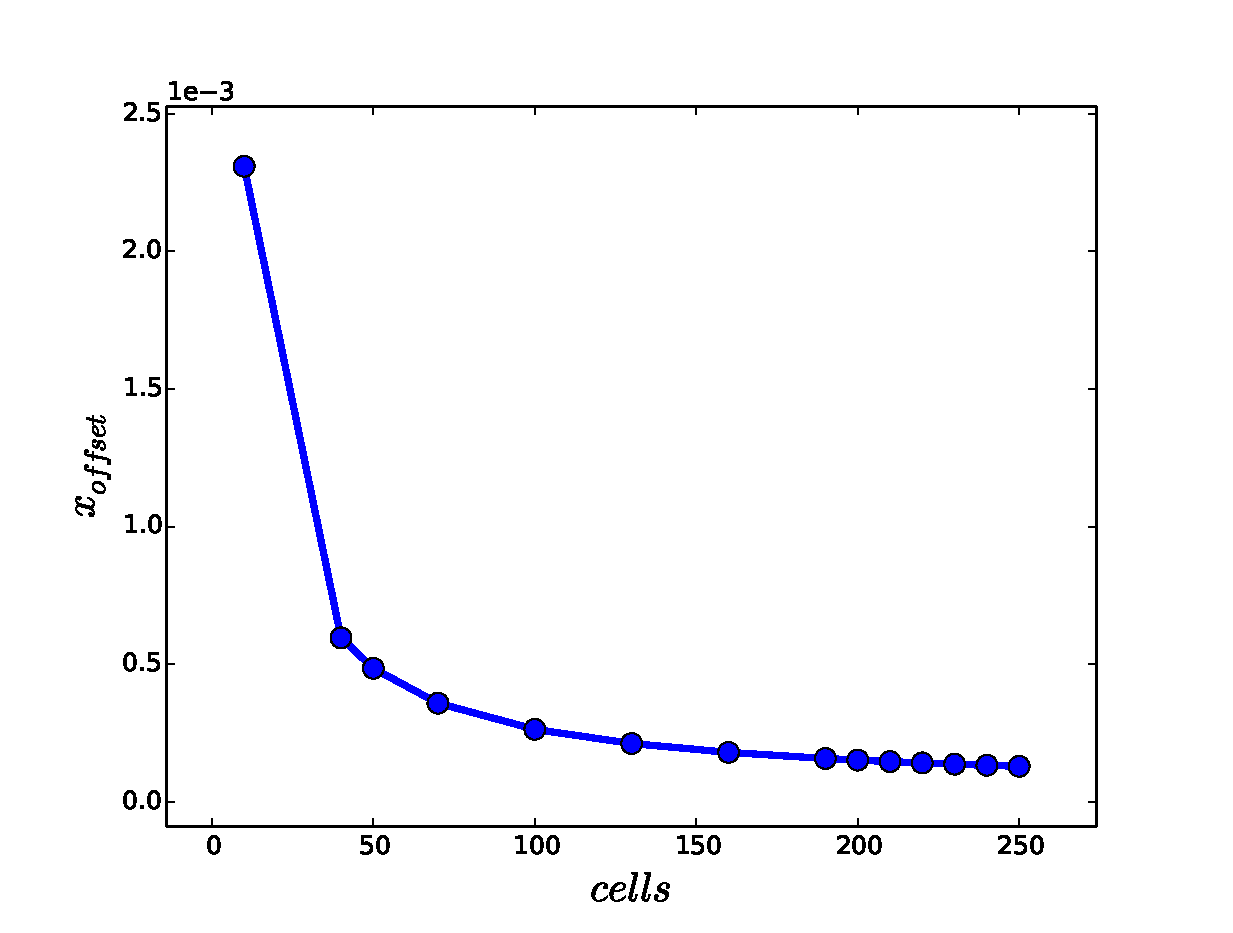
\includegraphics[width=\linewidth]{figures/cst-xs/mach-1p05/mass-diff-mach-1p05-x-offset.eps}
%    \caption{$x_{\text{\text{offset}}}$ vs. number of cells with mass conservation.}\label{fig:mass-diff-mach-1p05-x-offset}
%    \end{subfigure}
%    \begin{subfigure}{0.5\textwidth}
%    \centering
%    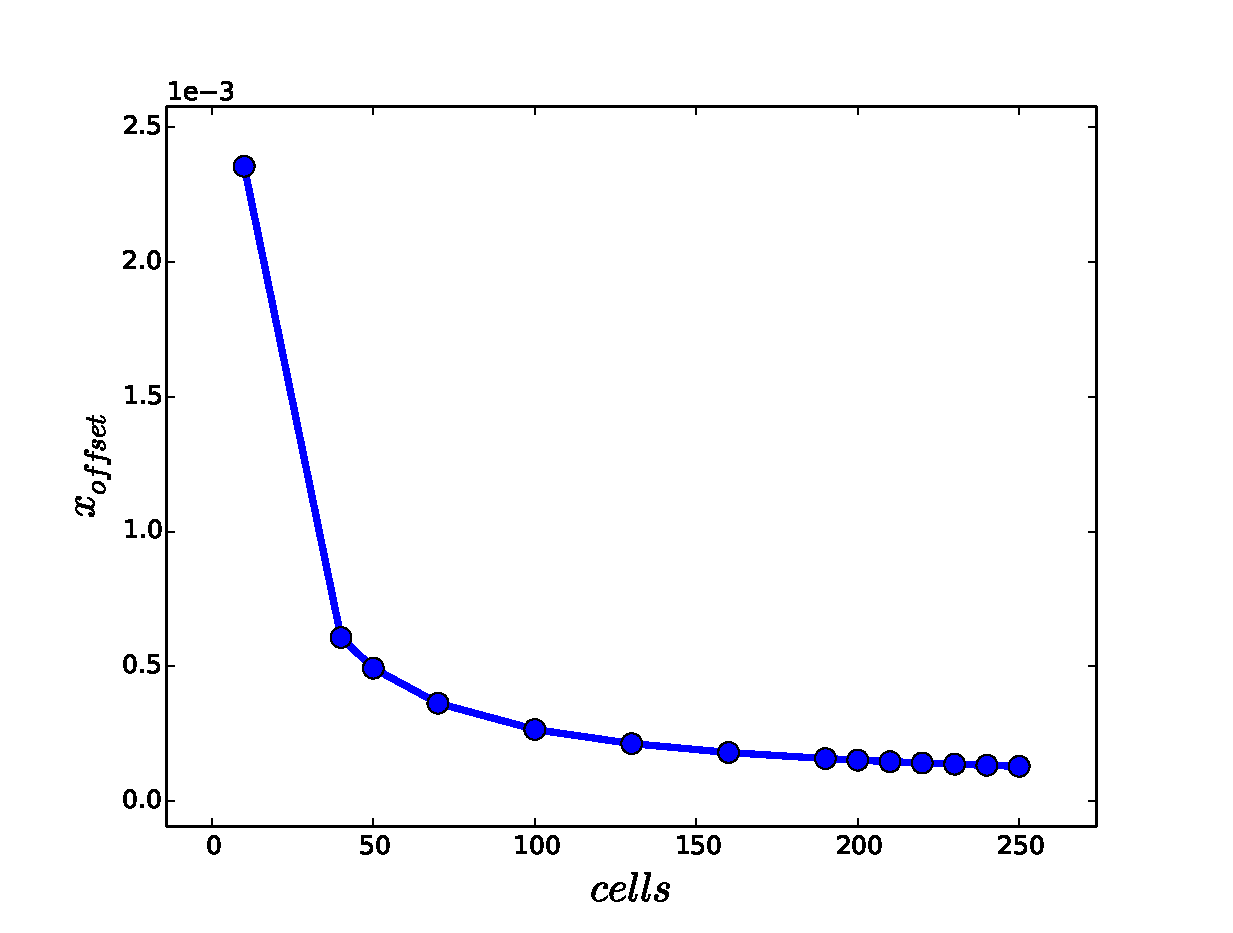
\includegraphics[width=\linewidth]{figures/cst-xs/mach-1p05/energy-diff-mach-1p05-x-offset.eps}
%    \caption{$x_{\text{\text{offset}}}$ vs. number of cells with total energy conservation.}\label{fig:energy-diff-mach-1p05-x-offset}
%    \end{subfigure}    
    \centering   
    \begin{subfigure}{0.49\textwidth}
    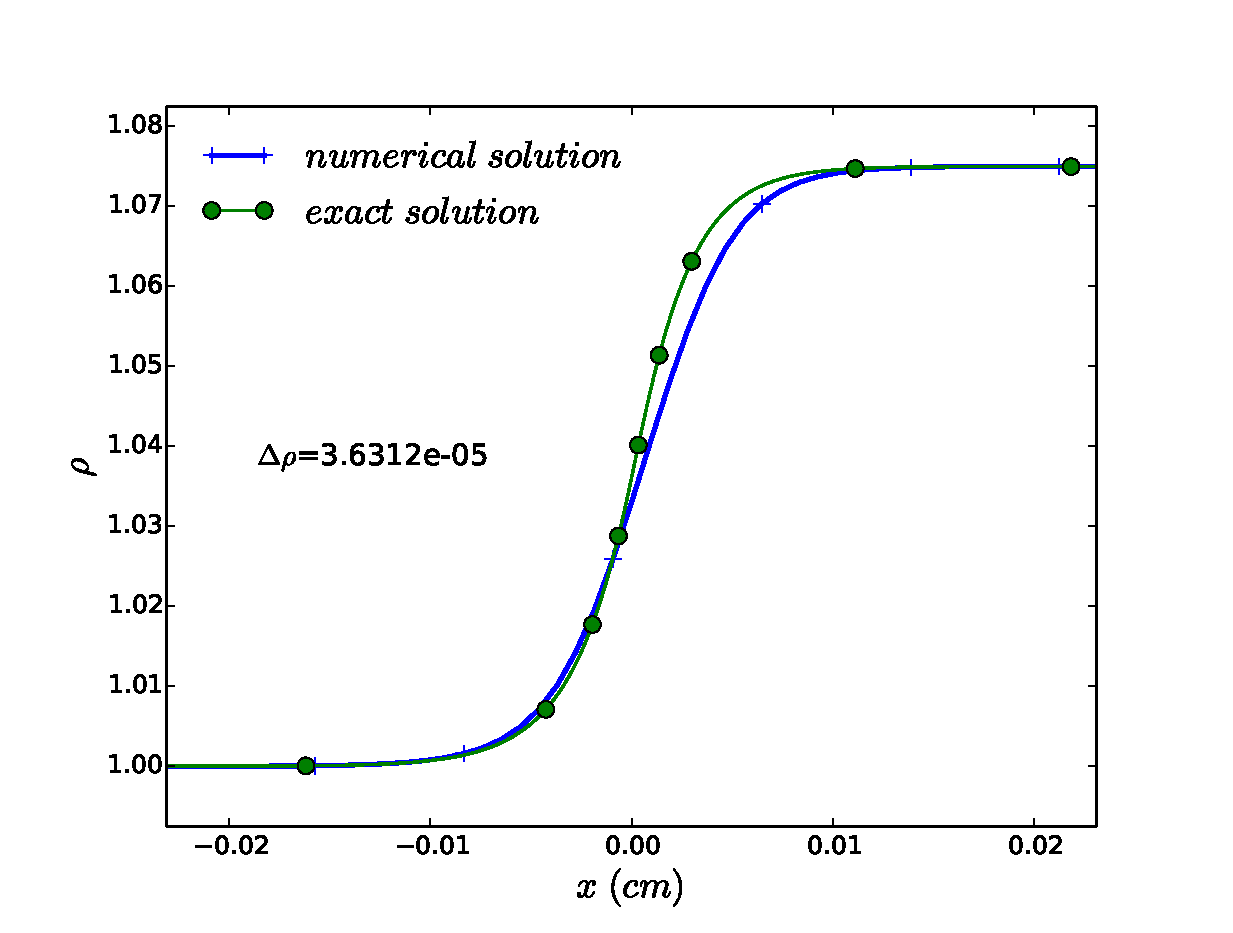
\includegraphics[width=\linewidth]{figures/cst-xs/mach-1p05/mach-1p05-density-nel-50-zero-shift.eps}
    \caption{}\label{fig:mach-1p05-cst-xs-density-no-shift}
    \end{subfigure}
    %
    \begin{subfigure}{0.49\textwidth}
    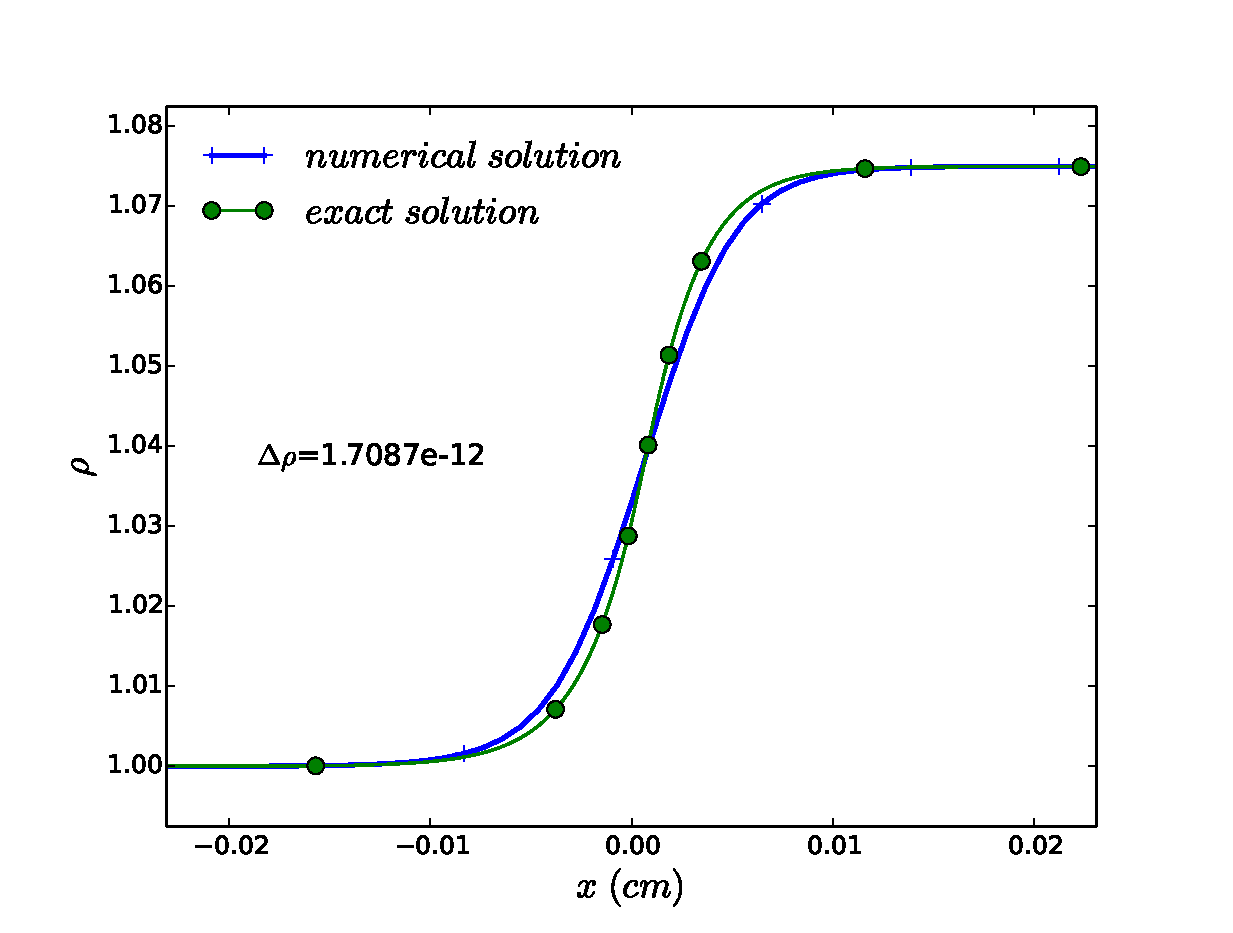
\includegraphics[width=\linewidth]{figures/cst-xs/mach-1p05/mach-1p05-density-nel-50-plot.eps}
    \caption{}\label{fig:mach-1p05-cst-xs-density-with-shift}
    \end{subfigure}
    \caption{Material density before (a) and after (b) shifting.}\label{fig:mach-1p05-shift-vs-non-shift}
\end{figure}
%
%\tcr{if you minimize the absolute value of the difference in mass, the figure 1.b still shows that the 2 solutions are not
%identical. why does that figure have a value of delta rho $=10^{-12}$. this doesn't look right} \tcb{This is consistent with equation 32 since there is no absolute value. It will, however, have to be changed}
The convergence rates for the material density, the material temperature, the radiation temperature and the mach number are given in \fig{fig:mach-1p05-cst-xs-conv} for the $L_1$ and $L_2$ error norms between the numerical and semi-analytical solutions for the variables $(\rho, T, \epsilon, Mach)$. A reference line of slope $2$ is also plotted which clearly shows that second-order accuracy is achieved in both the $L_1$ and $L_2$ error norms under mesh refinement with both mass and energy conservations. This example proves that the EVM achieves second-order accuracy for smooth solutions.
%and that the entropy condition still holds in the EDL as shown in \sct{sec:cons-equi-diff-limit}.
%
\begin{figure}[h]
    \begin{subfigure}{0.5\textwidth}
    \centering
    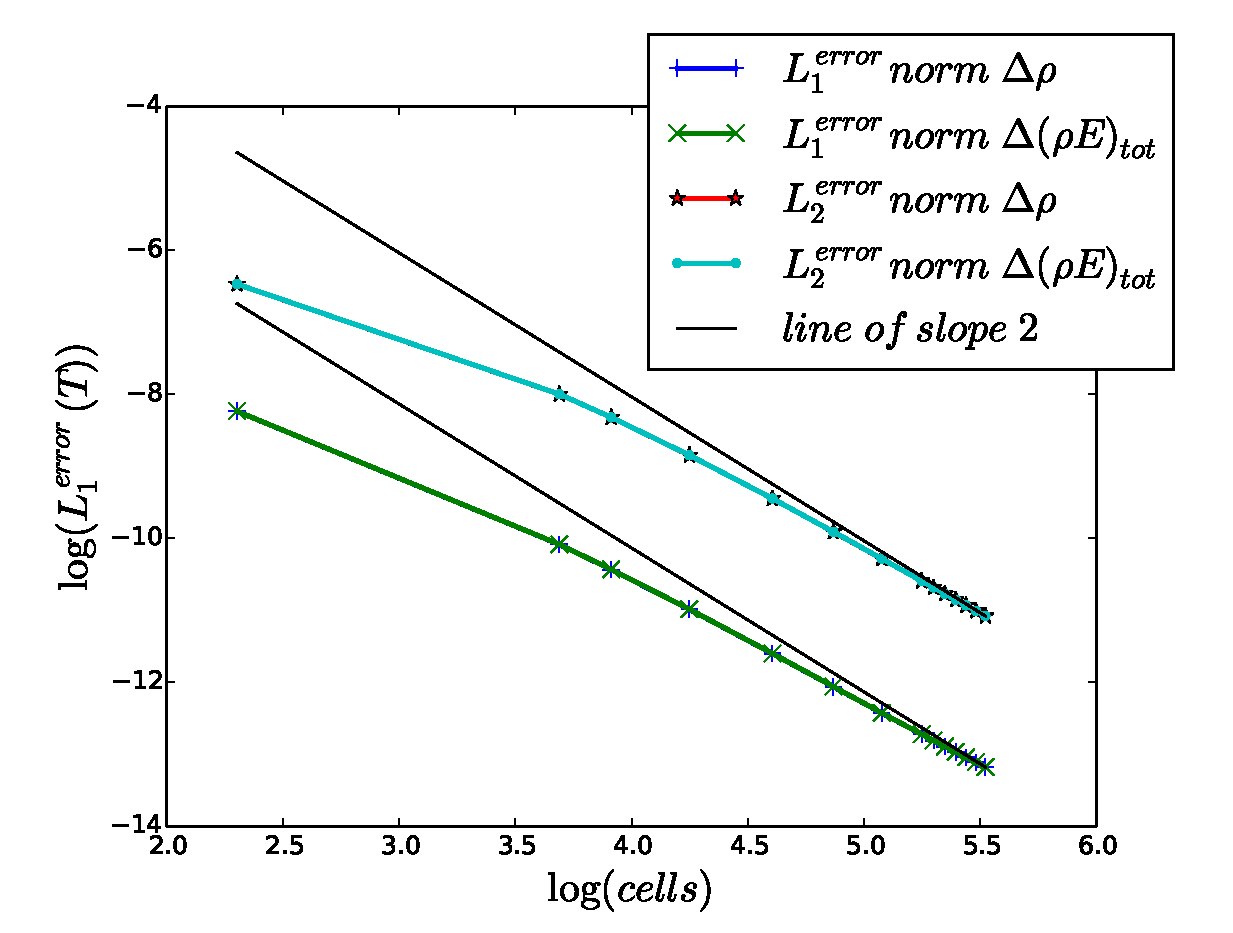
\includegraphics[width=\linewidth]{figures/cst-xs/mach-1p05/mass-energy-diff-mat-temp-convergence.eps}
    \caption{Material temperature.}\label{fig:mach-1p05-cst-xs-temp-conv}
    \end{subfigure}
    ~
    \begin{subfigure}{0.5\textwidth}
    \centering
    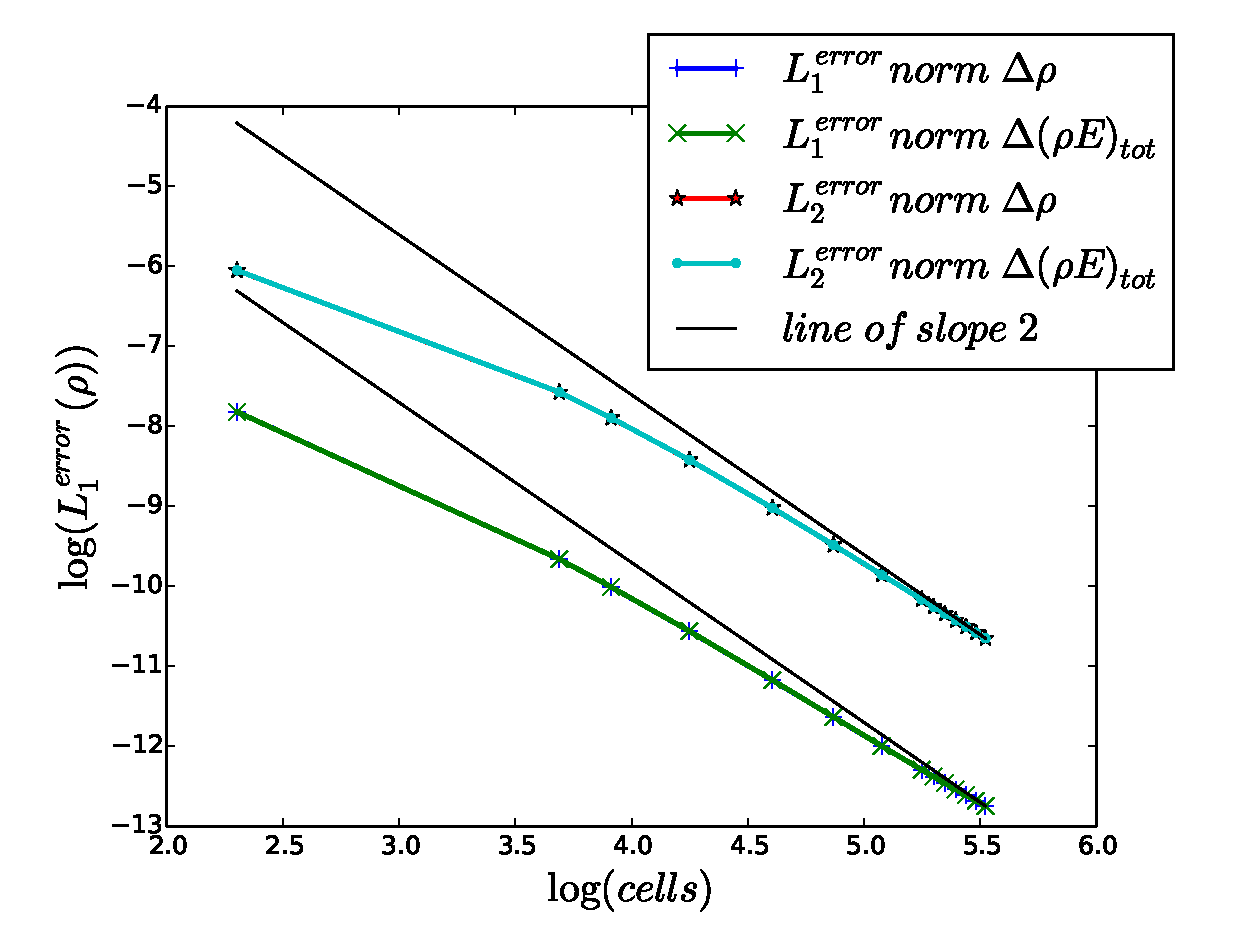
\includegraphics[width=\linewidth]{figures/cst-xs/mach-1p05/mass-energy-diff-density-convergence.eps}
    \caption{Material density.}\label{fig:mach-1p05-cst-xs-density-conv}
    \end{subfigure}
    
    \begin{subfigure}{0.5\textwidth}
    \centering
    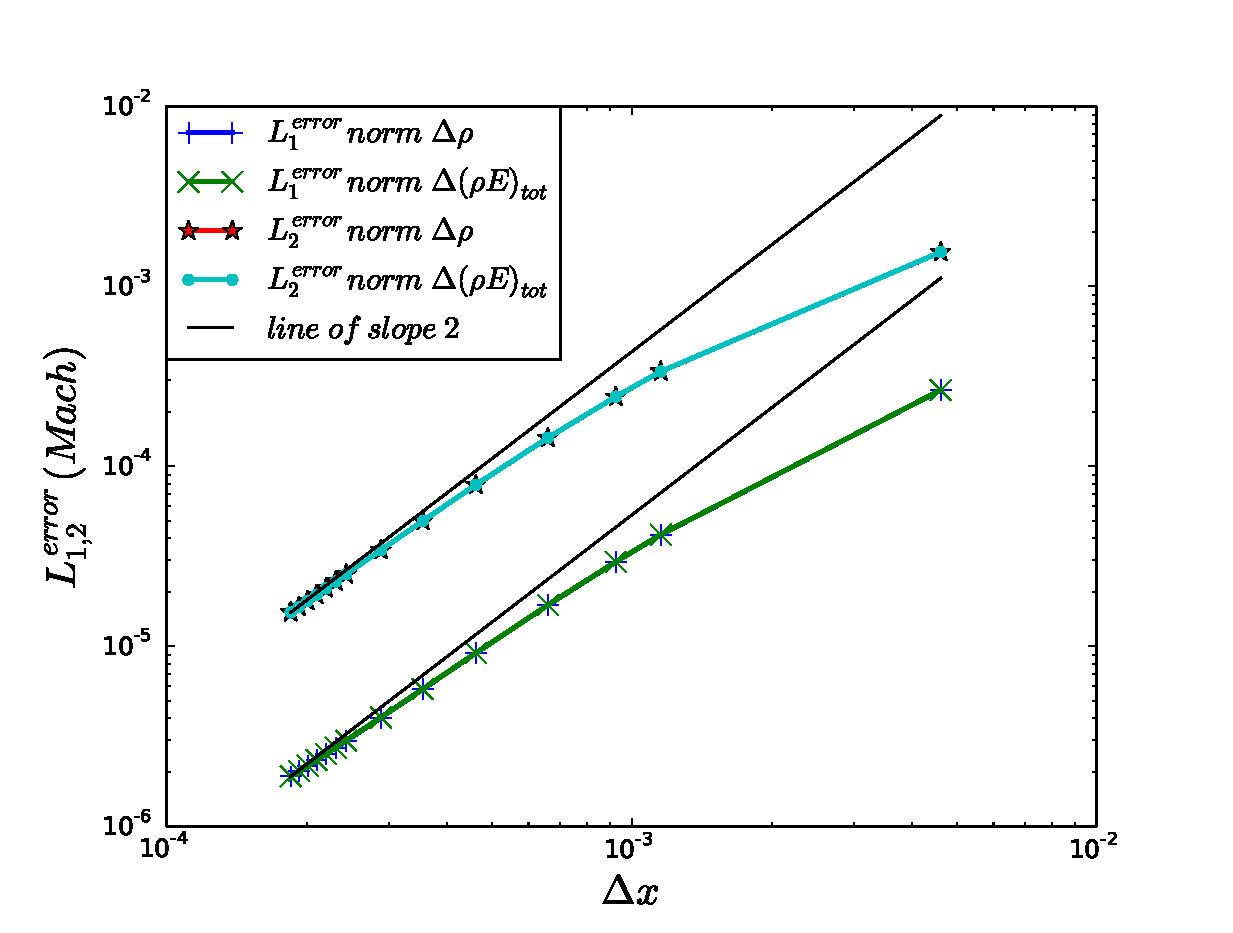
\includegraphics[width=\linewidth]{figures/cst-xs/mach-1p05/mass-energy-diff-mach-number-convergence.eps}
    \caption{Mach number.}\label{fig:mach-1p05-cst-xs-mach-conv}
    \end{subfigure}
    ~
    \begin{subfigure}{0.5\textwidth}
    \centering
    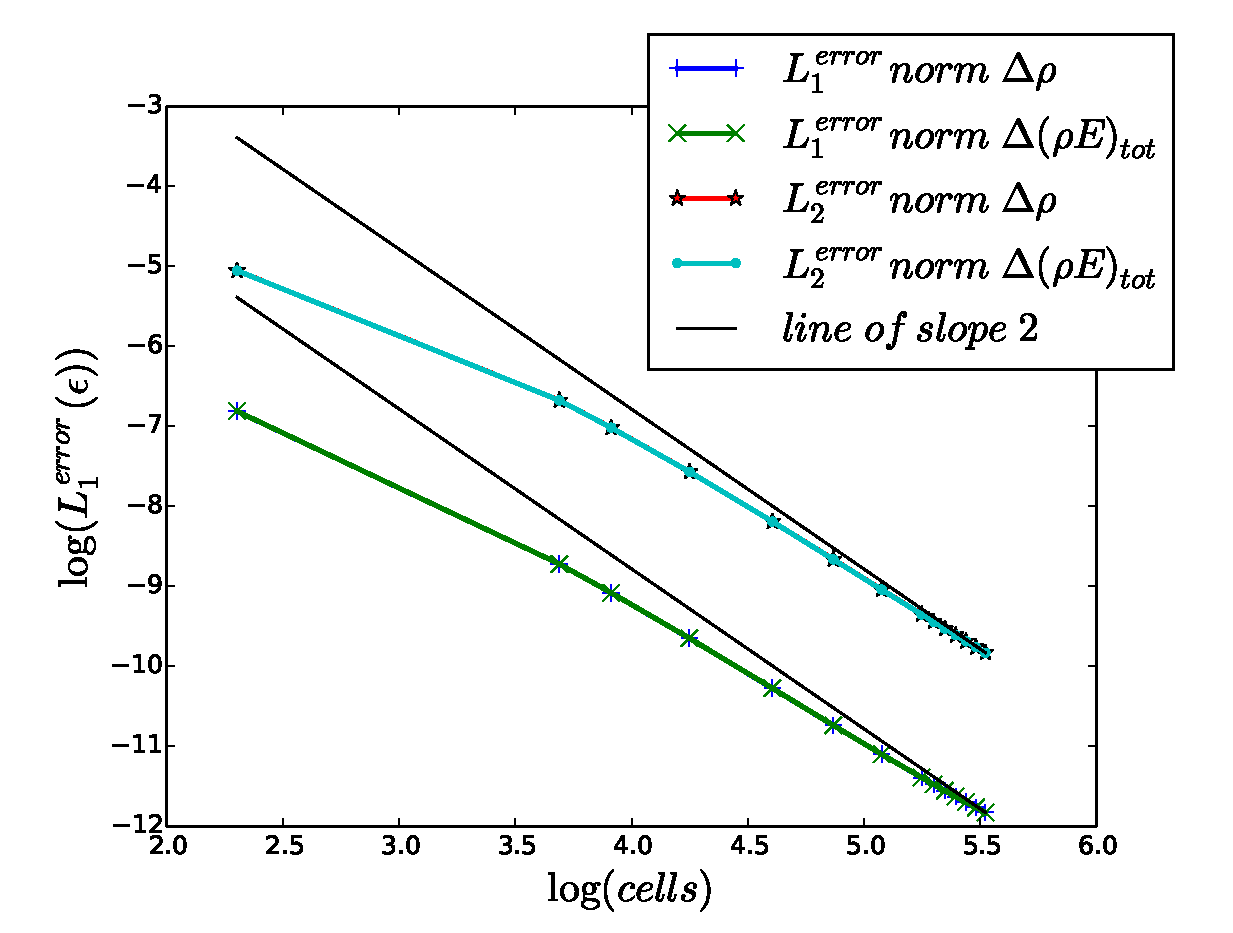
\includegraphics[width=\linewidth]{figures/cst-xs/mach-1p05/mass-energy-diff-radiation-convergence.eps}
    \caption{Radiation energy density.}\label{fig:mach-1p05-cst-xs-radiation-conv}
    \end{subfigure}        
\caption{Mach $1.05$ test: $L_1$ and $L_2$ error norms.}\label{fig:mach-1p05-cst-xs-conv}    
\end{figure}
%

The numerical and semi-analytical solutions of $(\rho, T, \epsilon, Mach)$ are plotted in \fig{fig:mach-1p05-cst-xs-density}, \fig{fig:mach-1p05-cst-xs-temp}, \fig{fig:mach-1p05-cst-xs-radiation} and \fig{fig:mach-1p05-cst-xs-mach}, respectively. We note that the numerical solution profiles are smooth and perfectly match the semi-analytical solutions for each variable. The viscosity coefficients $\kappa$ and $\kappa_\text{max}$ are plotted in \fig{fig:mach-1p05-cst-xs-visc} on a log scale. The entropy viscosity coefficient $\kappa$ is three to seven order of magnitude smaller than the first-order viscosity coefficient $\kappa_\text{max}$. Such behavior is expected as the numerical solution is smooth and the entropy production small.
%
\begin{figure}[h]
    \centering
    \begin{subfigure}{0.49\textwidth}
    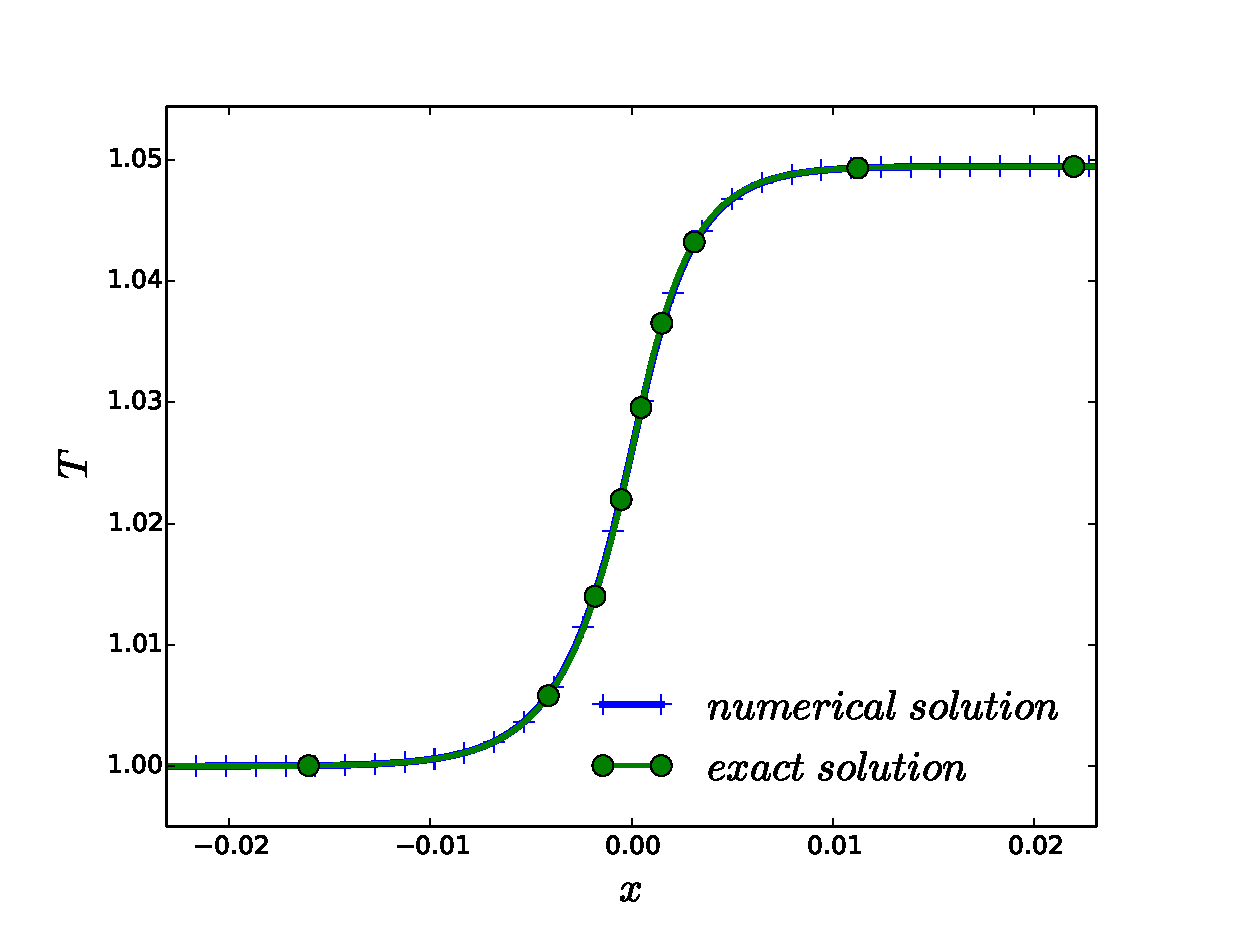
\includegraphics[width=\linewidth]{figures/cst-xs/mach-1p05/mass-diff-mach-1p05-mat-temp-nel-250-plot.eps}
    \caption{Material temperature.}\label{fig:mach-1p05-cst-xs-temp}
    \end{subfigure}
    \begin{subfigure}{0.49\textwidth}
    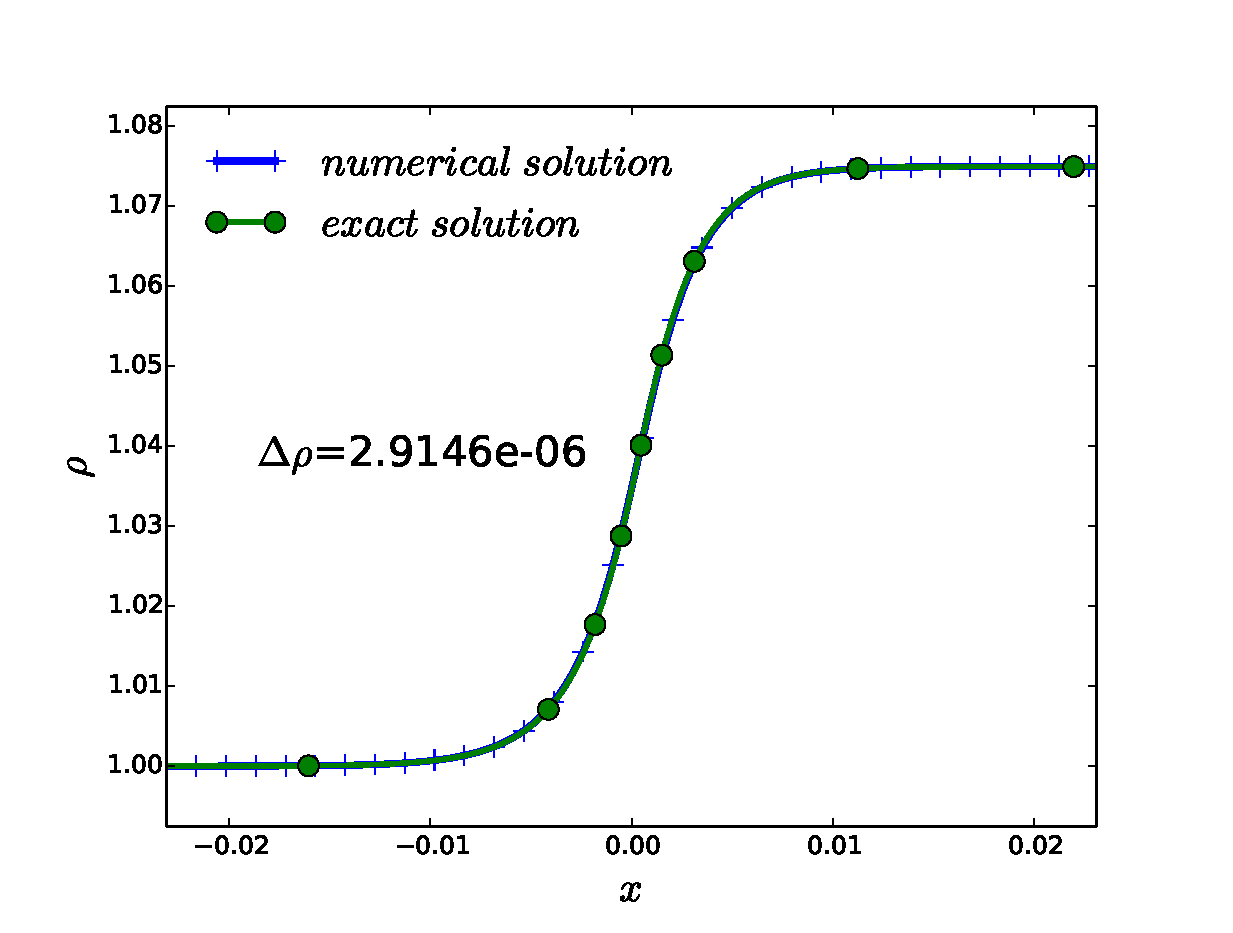
\includegraphics[width=\linewidth]{figures/cst-xs/mach-1p05/mass-diff-mach-1p05-density-nel-250-plot.eps}
    \caption{Material density.}\label{fig:mach-1p05-cst-xs-density}
    \end{subfigure}
    \begin{subfigure}{0.49\textwidth}
    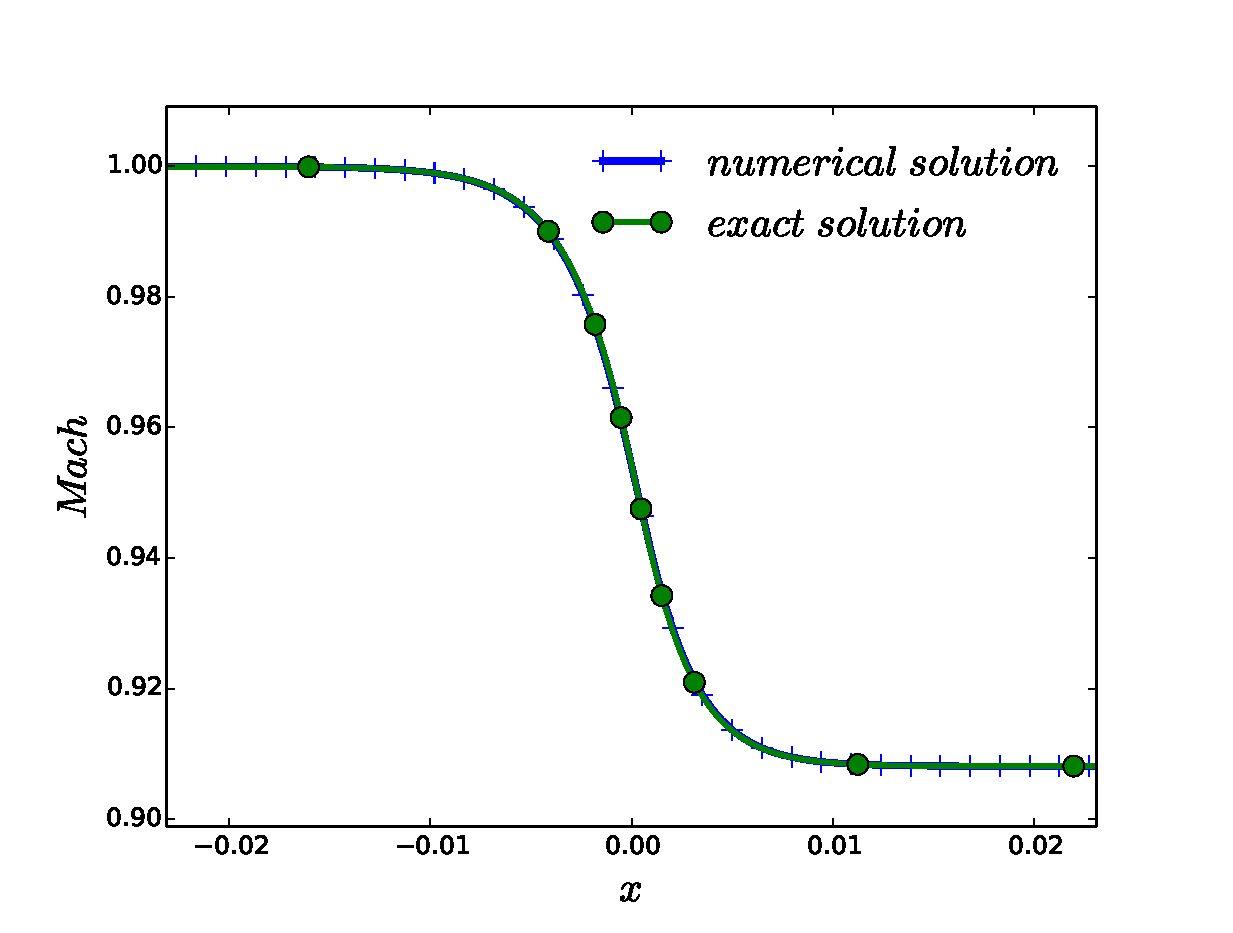
\includegraphics[width=\linewidth]{figures/cst-xs/mach-1p05/mass-diff-mach-1p05-mach-number-nel-250-plot.eps}
    \caption{Mach number.}\label{fig:mach-1p05-cst-xs-mach}
    \end{subfigure}
    \begin{subfigure}{0.49\textwidth}
    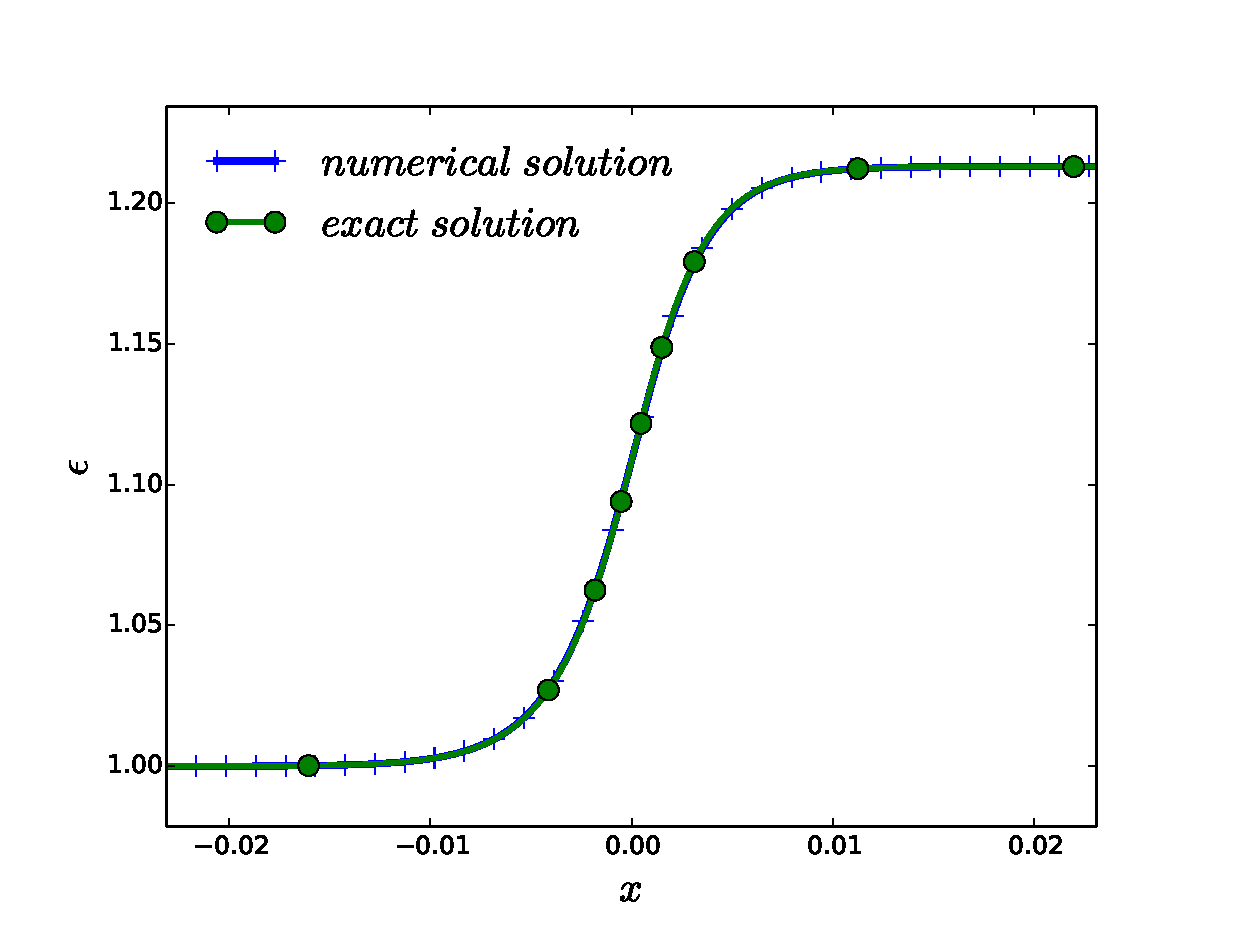
\includegraphics[width=\linewidth]{figures/cst-xs/mach-1p05/mass-diff-mach-1p05-radiation-nel-250-plot.eps}
    \caption{Radiation energy density.}\label{fig:mach-1p05-cst-xs-radiation}
    \end{subfigure}        
    \begin{subfigure}{0.49\textwidth}
    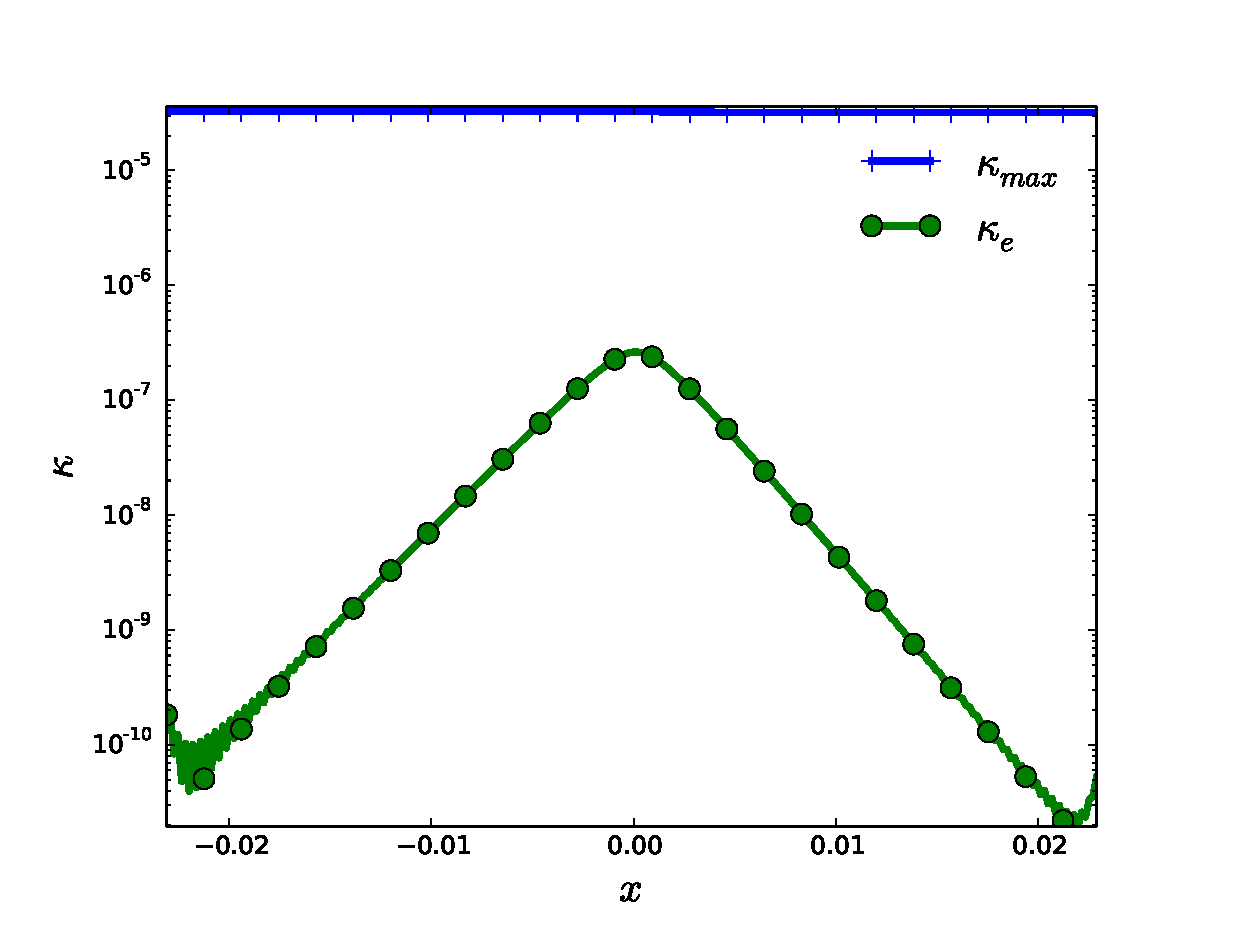
\includegraphics[width=\linewidth]{figures/cst-xs/mach-1p05/mass-diff-mach-1p05-visc-nel-250-plot.eps}
    \caption{Viscosity coefficients.}\label{fig:mach-1p05-cst-xs-visc}
    \end{subfigure}        
\caption{Mach $1.05$ test with constant opacity: Numerical ($250$ cells) and semi-analytical ($\sim 3500$ nodes) steady-state profiles;
material temperature (a), density (b), radiation energy (c), Mach number (d), and viscosity coefficient coefficient (e).}\label{fig:mach-1p05-cst-xs}    
\end{figure}
\FloatBarrier
\newpage
\pagebreak
\newpage

%------------------------------------------------------------------
\subsection{Mach-3 shock test with constant opacity}\label{sec:mach-3-cst-xs}
%------------------------------------------------------------------
%
For this test, the inlet Mach number is set to $3$ and the total and absorption opacities are still assumed constant. 
%\tcb{TO DELETE: The initial conditions and opacities are computed from the four non-dimensional numbers $\mathbb{P}_\infty=8.53 \cdot 10^{-5}$, $M=3$, $\mathbb{\Sigma}=10^6$ and $\mathbb{\Lambda}=1$ and is again found to be equal to $577.35 \ cm^{-1}$.} 
The code is run with a CFL condition of 1 until the steady-state solution is reached. The purpose of this test is twofold: (i) it shows that the EVM achieves first-order accuracy for numerical solutions with shocks, and, (ii) it illustrates the point made in \sct{sec:VR_new}, i.e., that the source terms positively contribute to the stabilization of the numerical solution.

A convergence study is performed for the variables $(\rho, T, \epsilon, Mach)$ by following the method given previous in \sct{sec:mthd-conv-test} on successively refined meshes with spatial mesh sizes ranging from $\sim 10^{-5}$ to $\sim 10^{-3}$ $cm$. The $L_1$ error norms computed with mass ($\Delta \rho$) and energy ($\Delta (\rho E)_{tot}$) conversation procedures are given in \fig{fig:mach-3-cst-xs-conv}; the semi-analytical solution used $5 \times 10^4$ nodes. A reference line of slope 1 shows that first-order convergence in the $L_1$ error is achieved for either conservation procedures. A convergence rate of 1 is expected for a numerical solution developing a shock \cite{lowrie-2009} 
(note that only convergence plots for the material temperature are provided in \cite{lowrie-2009}). 
We also note that in the pre-asymptotic range, the radiation energy variable exhibits second-order convergence, before leveling off
to a first-order convergence rate, see \fig{fig:mach-3-cst-xs-radiation-conv}.  
Given that the radiation energy variable is always smooth, even in the shock region, a higher convergence rate is possible
until the first-order rate present in the other (hydrodynamic) variables limits the energy radiation density rate to unity.
This behavior may warrant further analysis. 
%
\begin{figure}[ht]
    \begin{subfigure}{0.5\textwidth}
    \centering
    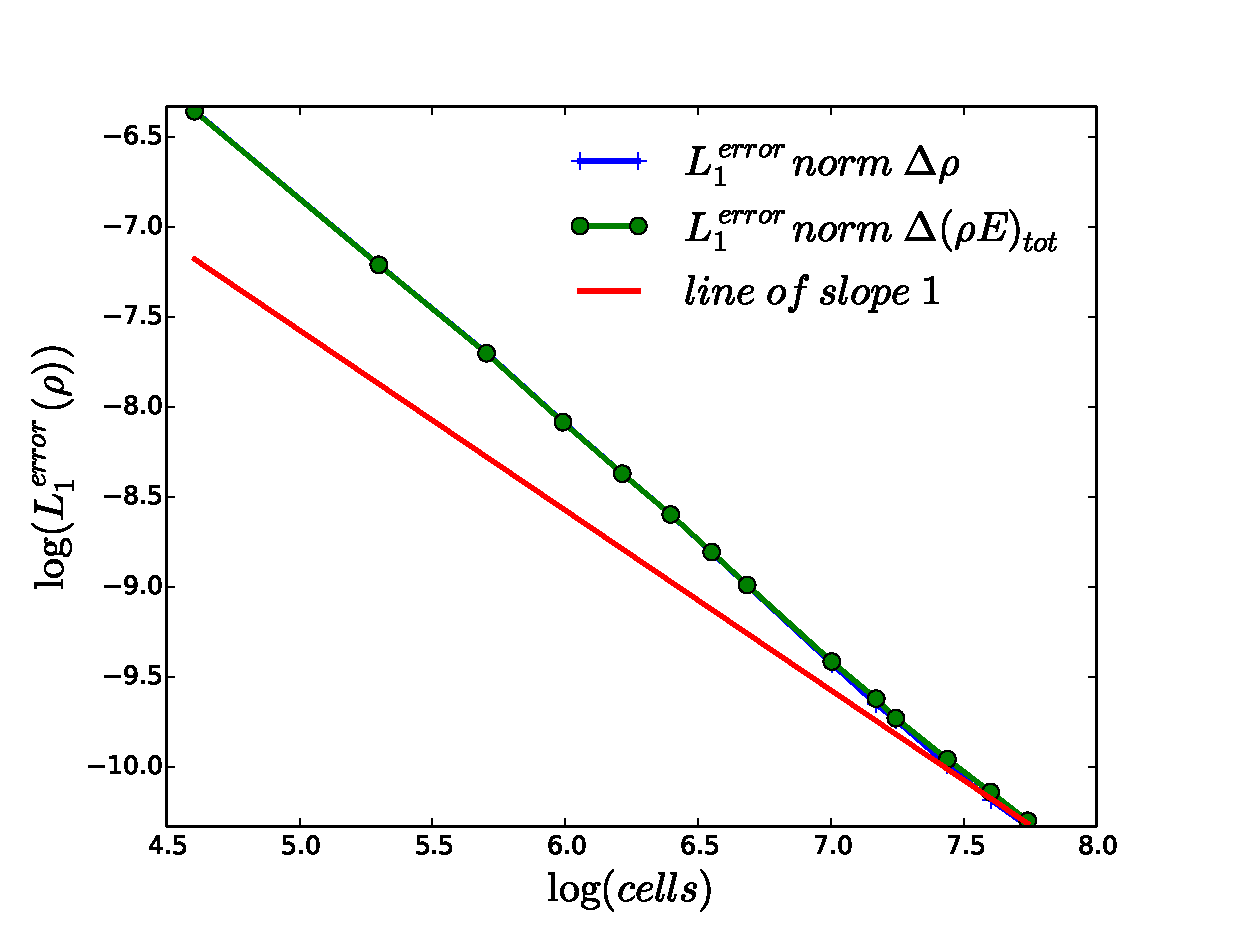
\includegraphics[width=\linewidth]{figures/cst-xs/mach-3/mass-energy-diff-scd-method-density-convergence.eps}
    \caption{Material density.}\label{fig:mach-3-cst-xs-density-conv}
    \end{subfigure}
    ~
    \begin{subfigure}{0.5\textwidth}
    \centering
    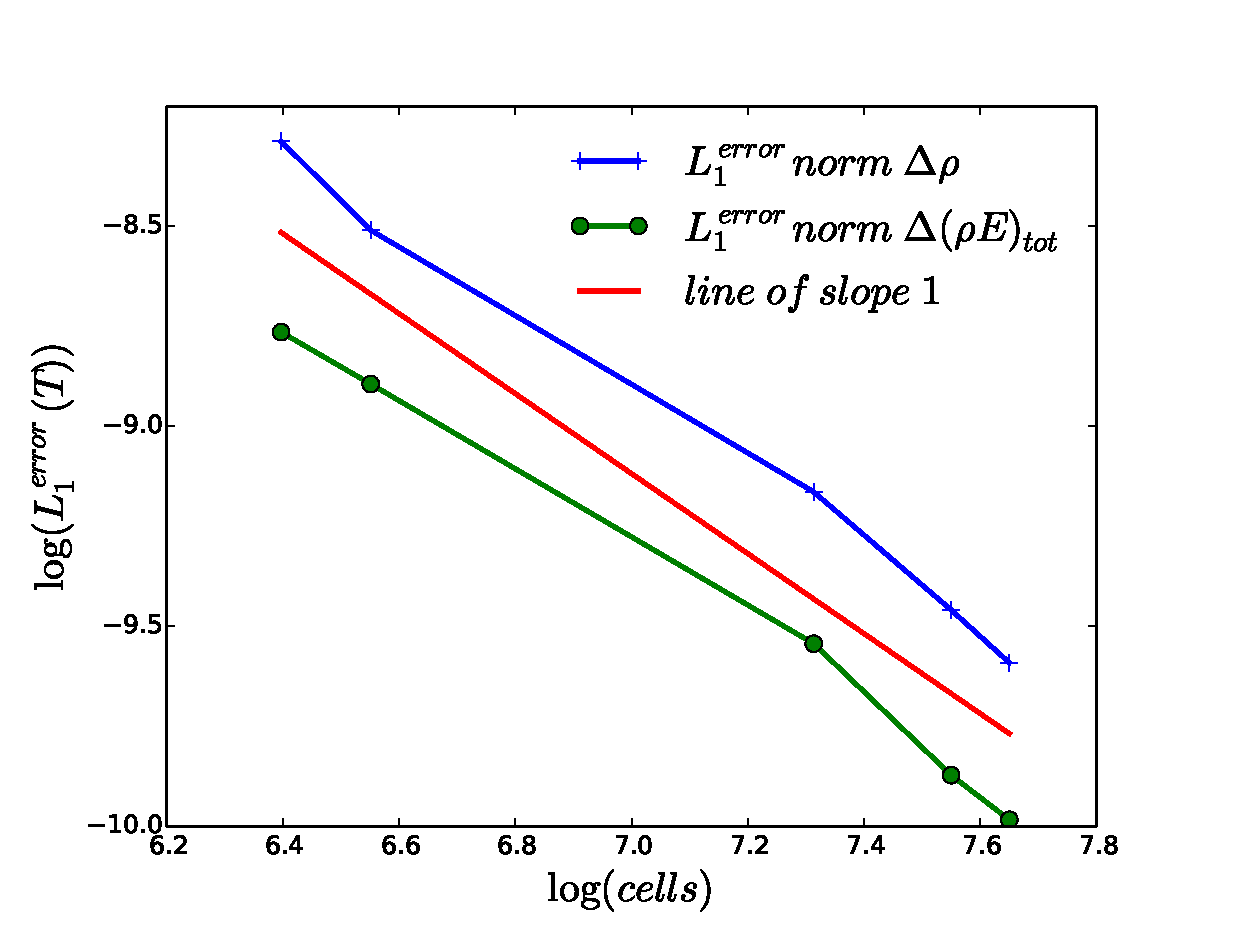
\includegraphics[width=\linewidth]{figures/cst-xs/mach-3/mass-energy-diff-scd-method-mat-temp-convergence.eps}
    \caption{Material temperature.}\label{fig:mach-3-cst-xs-temp-conv}
    \end{subfigure}
    
    \begin{subfigure}{0.5\textwidth}
    \centering
    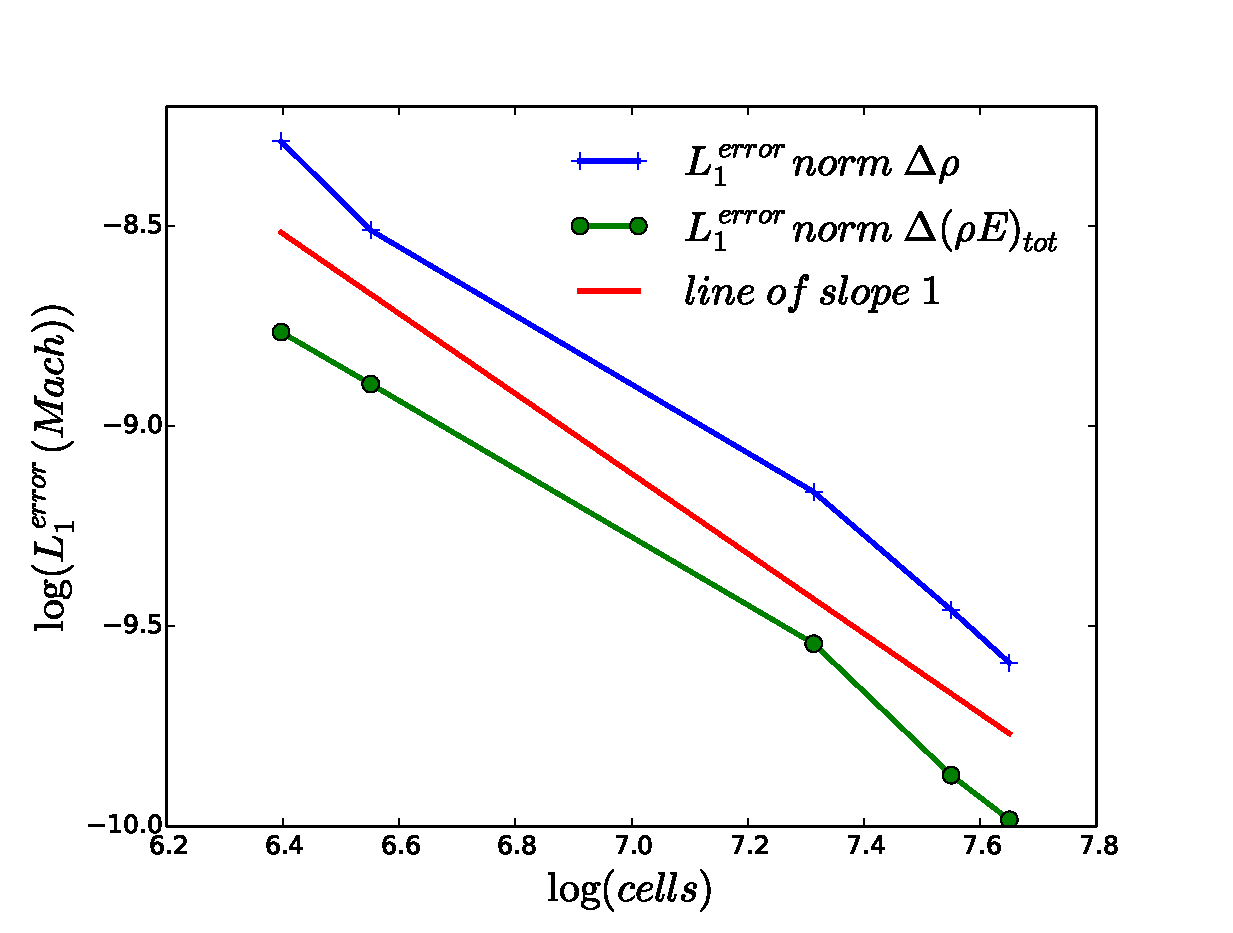
\includegraphics[width=\linewidth]{figures/cst-xs/mach-3/mass-energy-diff-scd-method-mach-number-convergence.eps}
    \caption{Mach number.}\label{fig:mach-3-cst-xs-mach-conv}
    \end{subfigure}
    ~
    \begin{subfigure}{0.5\textwidth}
    \centering
    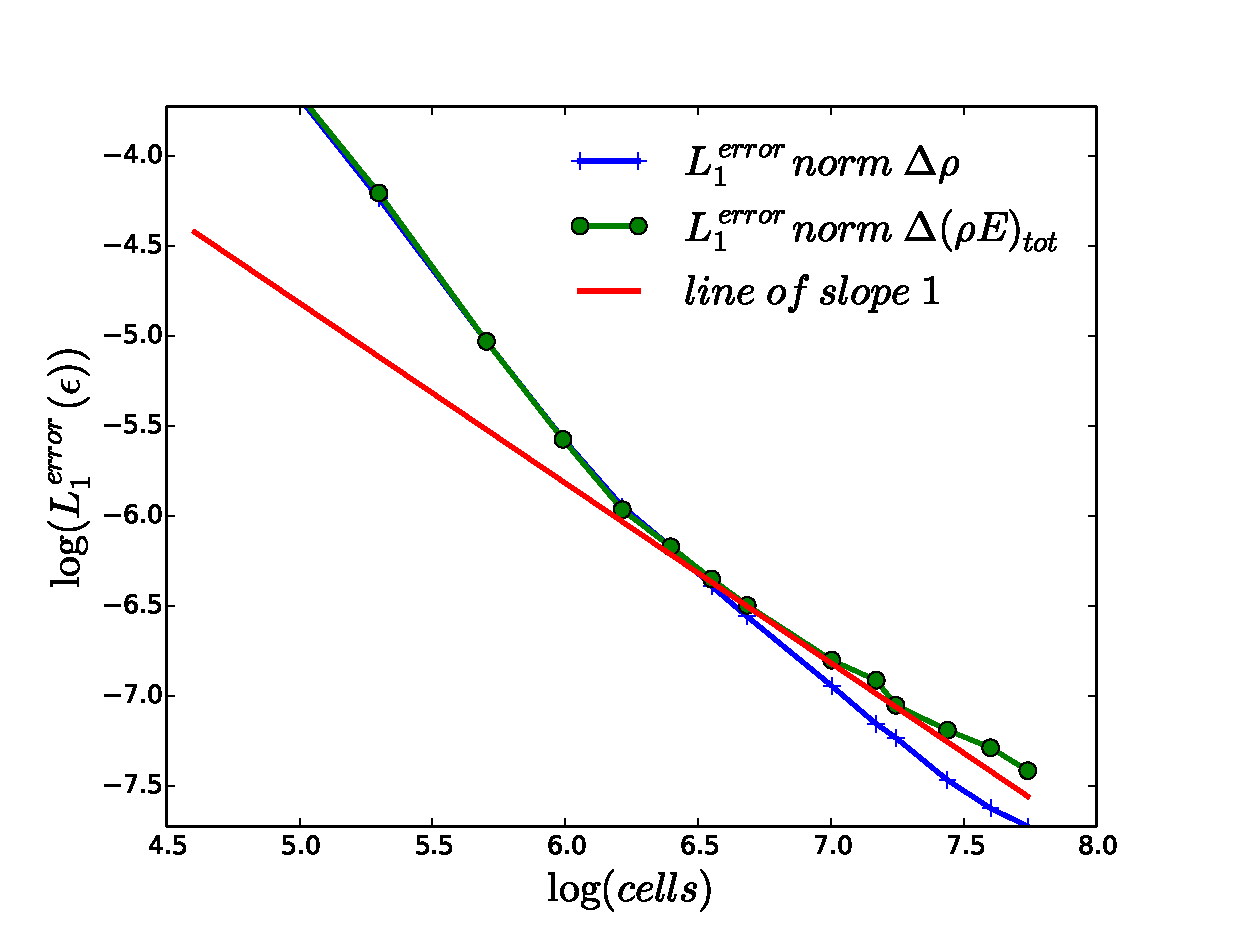
\includegraphics[width=\linewidth]{figures/cst-xs/mach-3/mass-energy-diff-scd-method-radiation-convergence.eps}
    \caption{Radiation energy density.}\label{fig:mach-3-cst-xs-radiation-conv}
    \end{subfigure}        
\caption{Mach $3$ test with constant opacity: $L_1$ error norms}\label{fig:mach-3-cst-xs-conv}    
\end{figure}
%

%<<<<<<< HEAD
The steady-state numerical results obtained with a spatial step size of $\Delta x \sim 10^{-4}$ $cm$ are plotted against the semi-analytical solutions %\cite{ferguson} \tcr{why cite ferguson here. shouldn't this have happened before?} \tcb{Well, I think he uses a new method so I will %check with him} \tcr{still not following the citation here. isn't Lowrie/Edwards? and why cite this here again, we cited it many times %before} 
along with the viscosity coefficients $\kappa$ and $\kappa_\text{max}$ in \fig{fig:mach-3-cst-xs}. All variables show good agreement with the semi-analytical solutions. A shock is located around $x=0$ in the material density and mach number profiles in \fig{fig:mach-3-cst-xs-dens} and \fig{fig:mach-3-cst-xs-mach}, respectively. The shock is well resolved and the numerical solution does not display any instabilities (over/undershoots). In \fig{fig:mach-3-cst-xs-temp}, the material temperature profile displays a Zeldovich's spike in the vicinity of the shock region: the spike is well resolved and matches the semi-analytical solution. On the other hand, the radiation energy density shown in \fig{fig:mach-3-cst-xs-rad} remains smooth even in the vicinity of the peak because of the diffusion term $ \partial_x \left( \frac{c}{3 \sigma_t} \partial_x \epsilon \right)$ in the radiation equation (\eqt{eq:GRHrad}). The viscosity coefficients $\kappa$ and $\kappa_\text{max}$ are plotted in \fig{fig:mach-3-cst-xs-visc} on a log scale. We observe that $\kappa$ is peaked in the vicinity of the shock and small elsewhere. This behavior is in agreement with the underlying principles invioked in the definition of the viscosity coefficient $\kappa$, that is, $\kappa$
should be proportional to the local entropy residual. We also note that the viscosity coefficient $\kappa$ does not saturate to the first-order viscosity coefficient $\kappa_\text{max}$ but still efficiently stabilizes the numerical solution. This is a consequence of the point explained in \sct{sec:VR_new} that highlights the entropy-producing effects, i.e., stabilizing effects, of the relaxation and the diffusion terms (see \eqt{eq:ineq_ent_eq}).
%=======
%The steady-state numerical results obtained with a mesh of $1000$ cells are plotted against the semi-analytical solutions \cite{ferguson} \tcr{why cite ferguson here. shouldn't this have happened before?} \tcb{Well, I think he uses a new method so I will check with him} along with the viscosity coefficients $\kappa$ and $\kappa_\text{max}$ in \fig{fig:mach-3-cst-xs}. All variables show good agreement with the semi-analytical solutions. A shock is located around $x=0$ in the material density and mach number profiles in \fig{fig:mach-3-cst-xs-dens} and \fig{fig:mach-3-cst-xs-mach}, respectively. The shock is well resolved and the numerical solution does not display any instabilities (over/undershoots). In \fig{fig:mach-3-cst-xs-temp}, the material temperature profile displays a Zeldovich spike in the vicinity of the shock region: the spike is well resolved and matches the semi-analytical solution. On the other hand, the radiation temperature shown in \fig{fig:mach-3-cst-xs-rad} remains smooth even in the vicinity of the peak because of the diffusion term $ \partial_x \left( \frac{c}{3 \sigma_t} \partial_x \epsilon \right)$ in the radiation equation (\eqt{eq:GRHrad}). The viscosity coefficients $\kappa$ and $\kappa_\text{max}$ are plotted in \fig{fig:mach-3-cst-xs-visc} on a log scale. We observe that $\kappa$ is peaked in the vicinity of the shock and small elsewhere. This behavior is conformed to the definition of the viscosity coefficient $\kappa$ that is set proportional to the local entropy residual. We also note that the viscosity coefficient $\kappa$ does not saturate to the first-order viscosity coefficient $\kappa_\text{max}$ but still efficiently stabilizes the numerical solution. This is a consequence of the point explained in \sct{sec:ent-cond-full-GRH} that highlights the entropy-producing effects, i.e., stabilizing effects, of the relaxation and the diffusion terms (see \eqt{eq:ineq_ent_eq}). 
%>>>>>>> 80a5074596b6d65166c9c071f44d3b9efb860727
Consequently, the relaxation and diffusion terms participate in stabilizing the numerical solution along with the EVM.
%
\begin{figure}[h]
    \centering
    \begin{subfigure}{0.49\textwidth}
    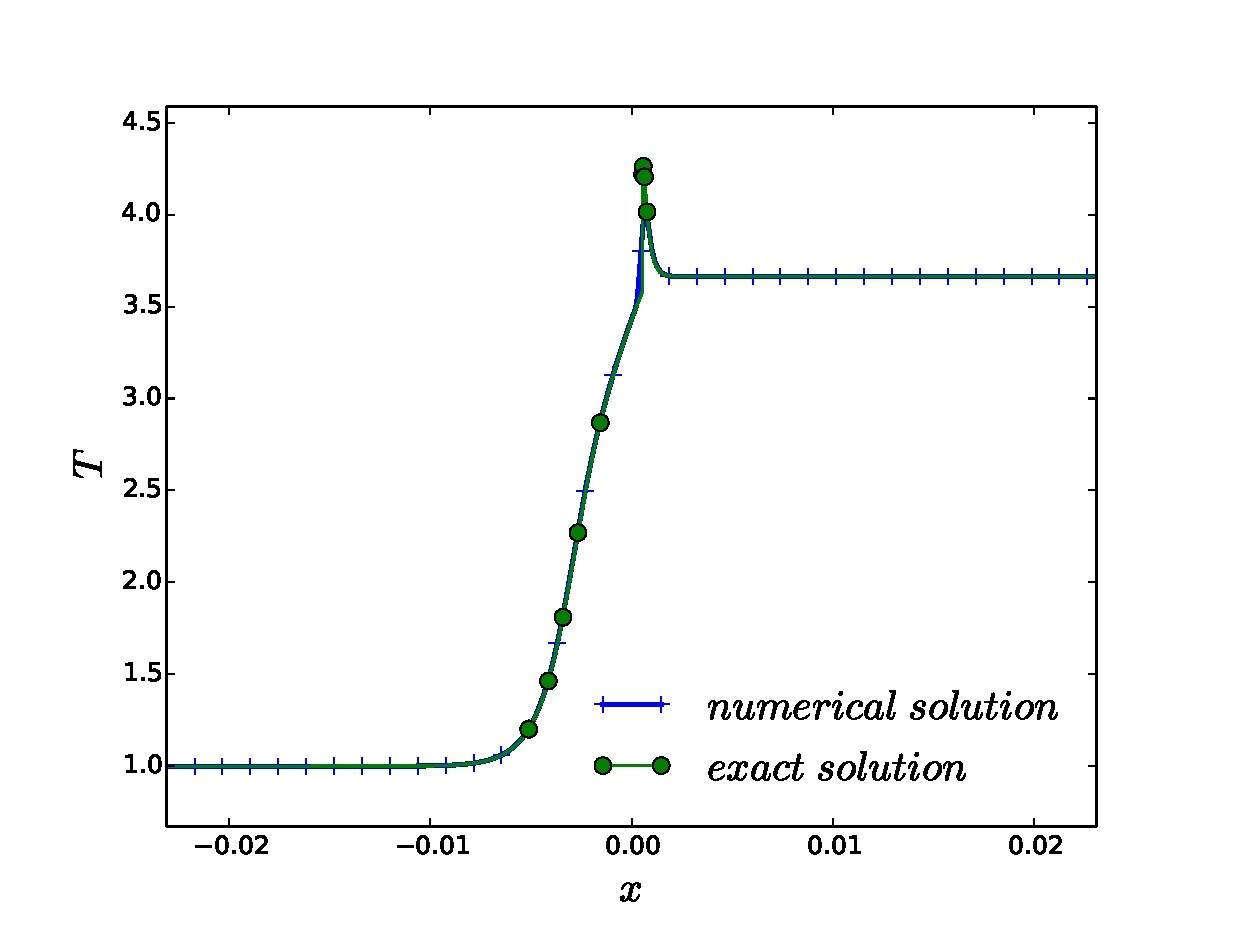
\includegraphics[width=\linewidth]{figures/cst-xs/mach-3/mass-diff-mat-temp-nel-1000-plot.eps}
    \caption{Material temperature.}\label{fig:mach-3-cst-xs-temp}
    \end{subfigure}	
%
    \begin{subfigure}{0.49\textwidth}
    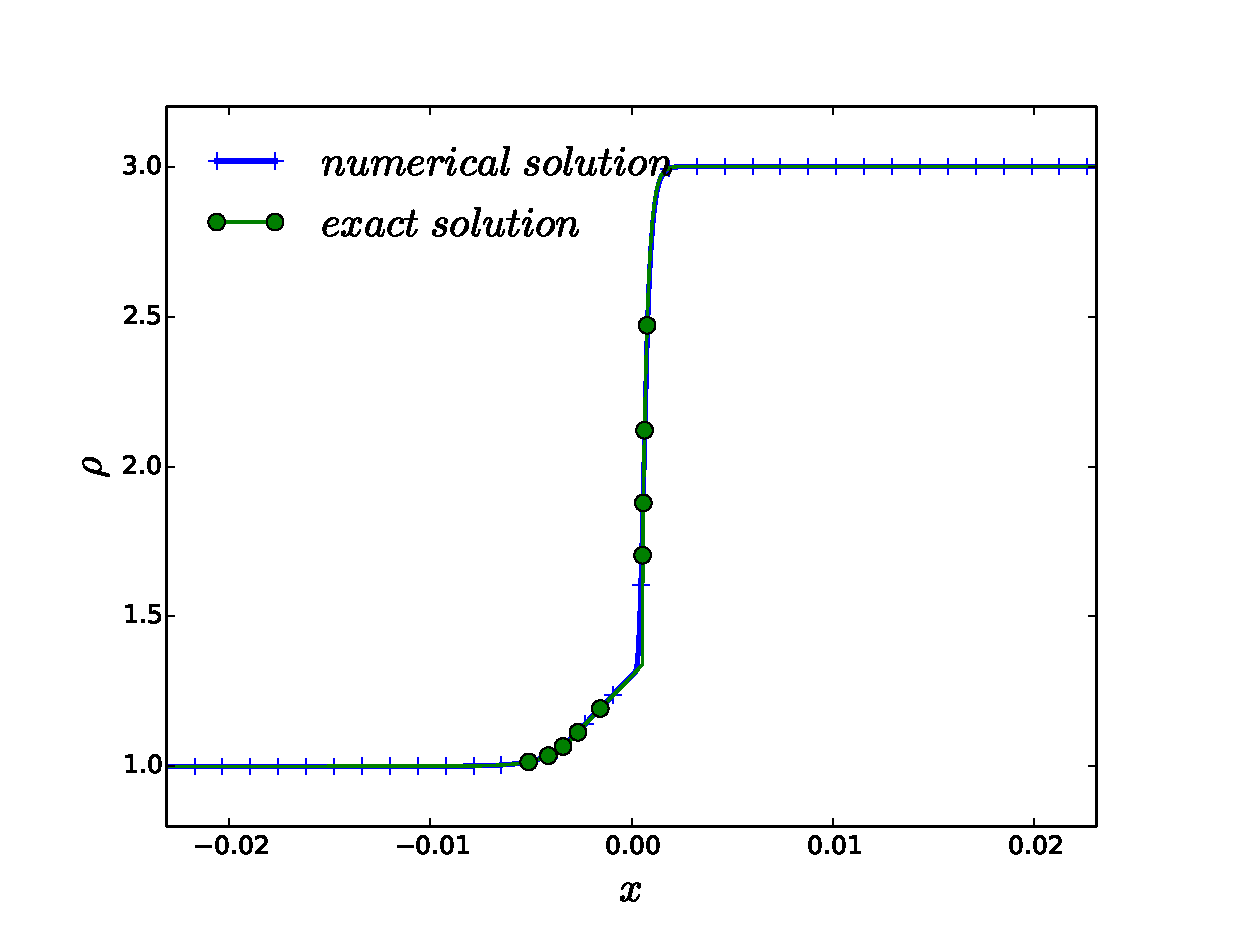
\includegraphics[width=\linewidth]{figures/cst-xs/mach-3/mass-diff-density-nel-1000-plot.eps}
    \caption{Material density.}\label{fig:mach-3-cst-xs-dens}
    \end{subfigure}
%
    \begin{subfigure}{0.49\textwidth}
    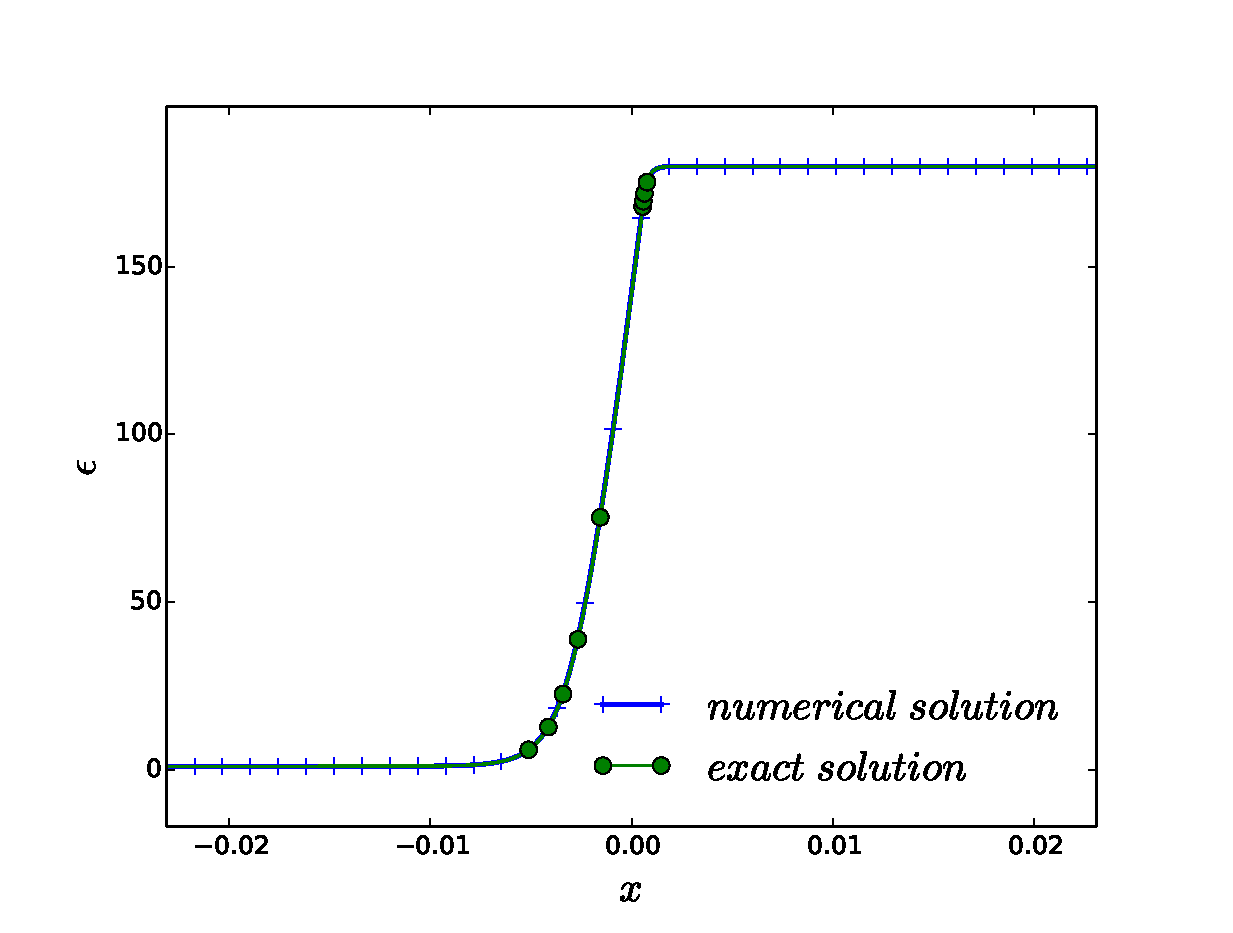
\includegraphics[width=\linewidth]{figures/cst-xs/mach-3/mass-diff-radiation-nel-1000-plot.eps}
    \caption{Radiation energy density.}\label{fig:mach-3-cst-xs-rad}
    \end{subfigure}
%   
    \begin{subfigure}{0.49\textwidth}
    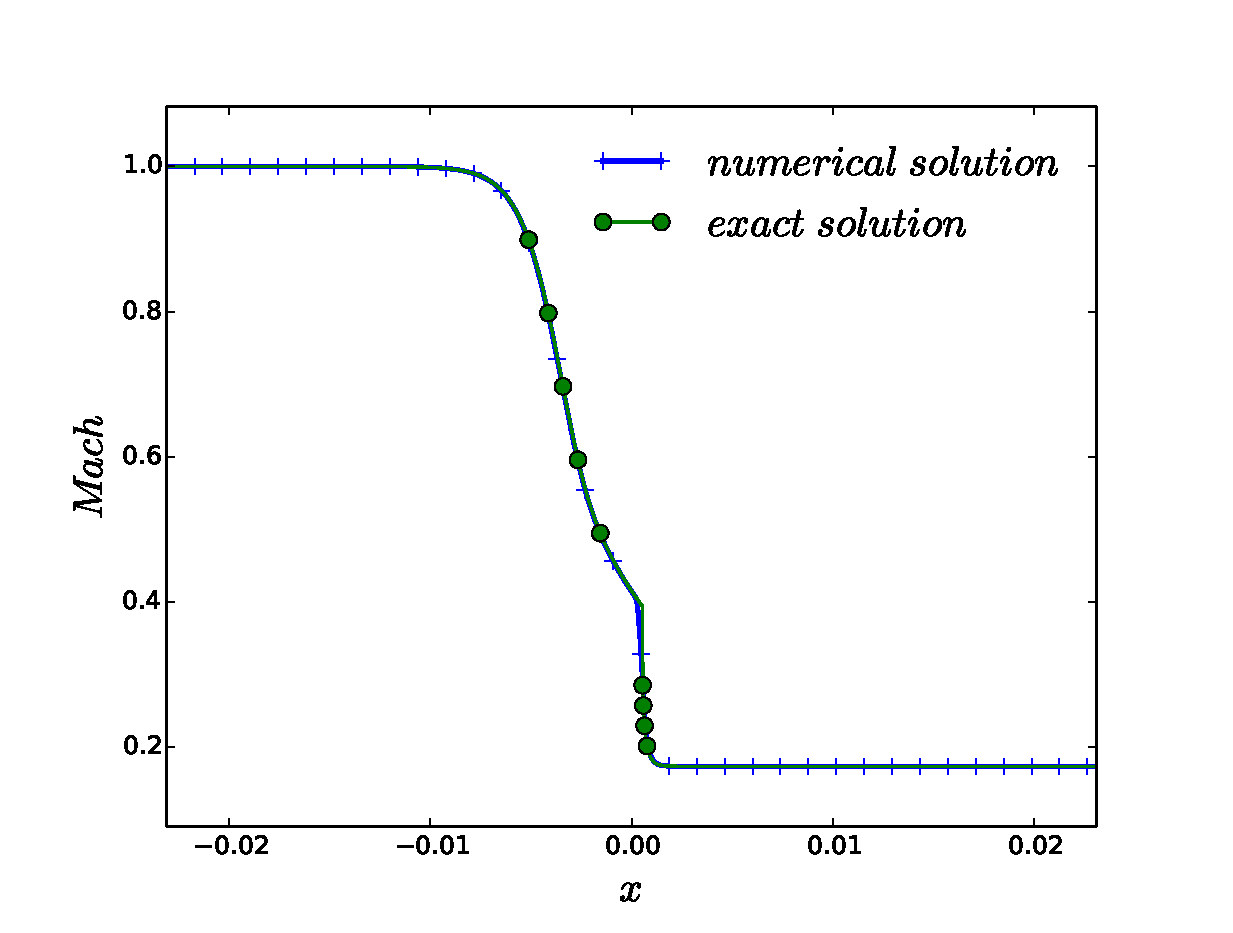
\includegraphics[width=\linewidth]{figures/cst-xs/mach-3/mass-diff-mach-number-nel-1000-plot.eps}
    \caption{Mach number.}\label{fig:mach-3-cst-xs-mach}
    \end{subfigure}
%
    \begin{subfigure}{0.49\textwidth}
    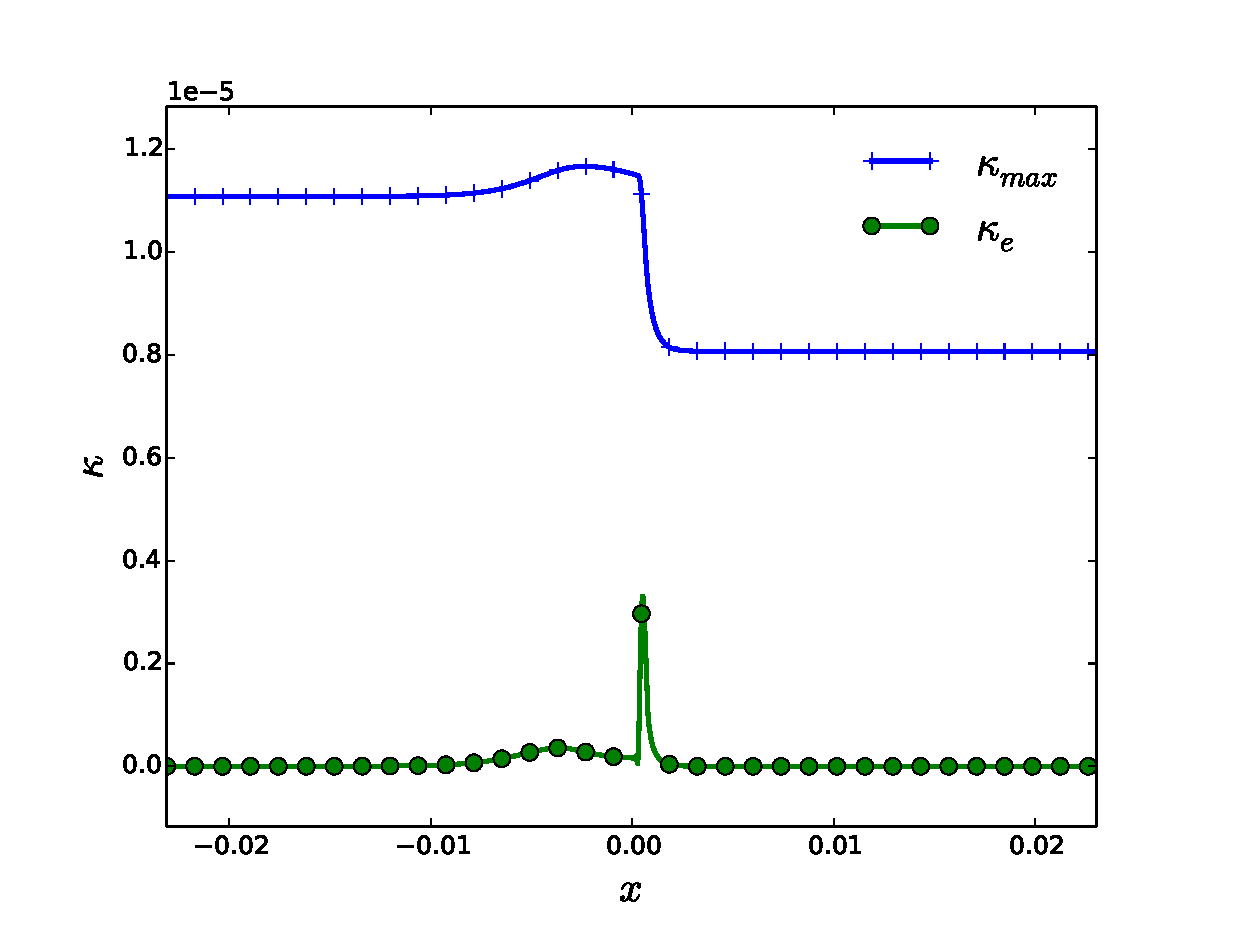
\includegraphics[width=\linewidth]{figures/cst-xs/mach-3/mass-diff-visc-nel-1000-plot.eps}
    \caption{Artificial viscosity coefficients.}\label{fig:mach-3-cst-xs-visc}
    \end{subfigure}        
\caption{Mach $3$ test with constant opacity: Numerical ($1000$ cells) and semi-analytical ($\sim 5 \cdot 10^4$ nodes) steady-state profiles for the material temperature (a),  density (b),  radiation temperature (c), Mach number (d), and  viscosity coefficient (e).}\label{fig:mach-3-cst-xs}      
\end{figure}
%

%------------------------------------------------------------------
\subsection{Mach-3 shock test with temperature-dependent opacity}\label{sec:mach-3-no-cst-xs}
%------------------------------------------------------------------
%
%\tcb{We need a reference for this test. I have the report that was emailed by Dr Morel to me but I am not sure this is sufficient} \\
%\tcb{I am not done with this part} \tcr{still?} \tcb{I am done with the text. Still missing the convergence plots as some of the simulations are still running} \\
We now consider a Mach 3 test in a pure absorber material with the same initial conditions as in \sct{sec:mach-3-cst-xs} but with an opacity that depends on the a-dimensional material properties, i.e., density $\hat{\rho}$ and temperature $\hat{T}$. An expression of the \emph{dimensional} form of the density- and  temperature-dependent opacity is given in \eqt{eq:opacity}:
% there was a tilde sigma here, why?
%
\begin{equation}\label{eq:opacity}
\sigma_a(\hat{\rho},\hat{T}) = \sigma_t(\hat{\rho},\hat{T}) = \hat{\rho} \frac{577.35}{\hat{T}^{3.5}} \ cm^{-1}\, .
\end{equation}
%
This simulation aims at exercising the entropy viscosity method with an opacity function that exhibits strong variations in the shock region. From a theoretical perspective, as shown in \sct{sec:VR_new}, the entropy inequality holds, meaning that the viscous regularization should efficiently stabilize any discontinuity or shock that may form in the numerical solution. 

Once again, a convergence study at steady state in the $L_1$ error norm is performed for the variables $(\rho, T, \epsilon, Mach)$ and plots are shown in \fig{fig:mach-3-dpt-xs-conv} . A reference line of slope 1 shows that first-order convergence in the $L_1$ error norm is achieved for all variables, as expected for a numerical solution containing a shock. Here again, the radiation energy density convergence rate in \fig{fig:mach-3-dpt-xs-radiation-conv} displays a higher convergence rate in pre-asymptotic region, i.e. the radiation energy density achieves second-order accuracy for $\Delta x \geq 10^{-4}$ even though the material variables are only first-order accurate. 
Numerical results for the material density, the material temperature and the radiation energy density are plotted against semi-analytical solutions in \fig{fig:mach-3-dpt-xs-dens}, \fig{fig:mach-3-dpt-xs-mat-temp} and \fig{fig:mach-3-dpt-xs-rad-temp}, respectively. We also provide plots of the viscosity coefficient profiles at steady state in \fig{fig:mach-3-dpt-xs-visc} and the opacity in \fig{fig:mach-3-dpt-xs-xs}.
%\begin{itemize}
%\item numerical results using definition of the viscosity coefficient provided in previous section: density, temperature, opacity and viscosity coefficient profiles.
%\item eyeball convergence study when refining the mesh.
%\item investigate the influence of the jumps in the definition of the viscosity coefficients: run the same numerical test with and without jumps.
%\end{itemize}
%
\begin{figure}[ht]
    \centering
    \begin{subfigure}{0.49\textwidth}
    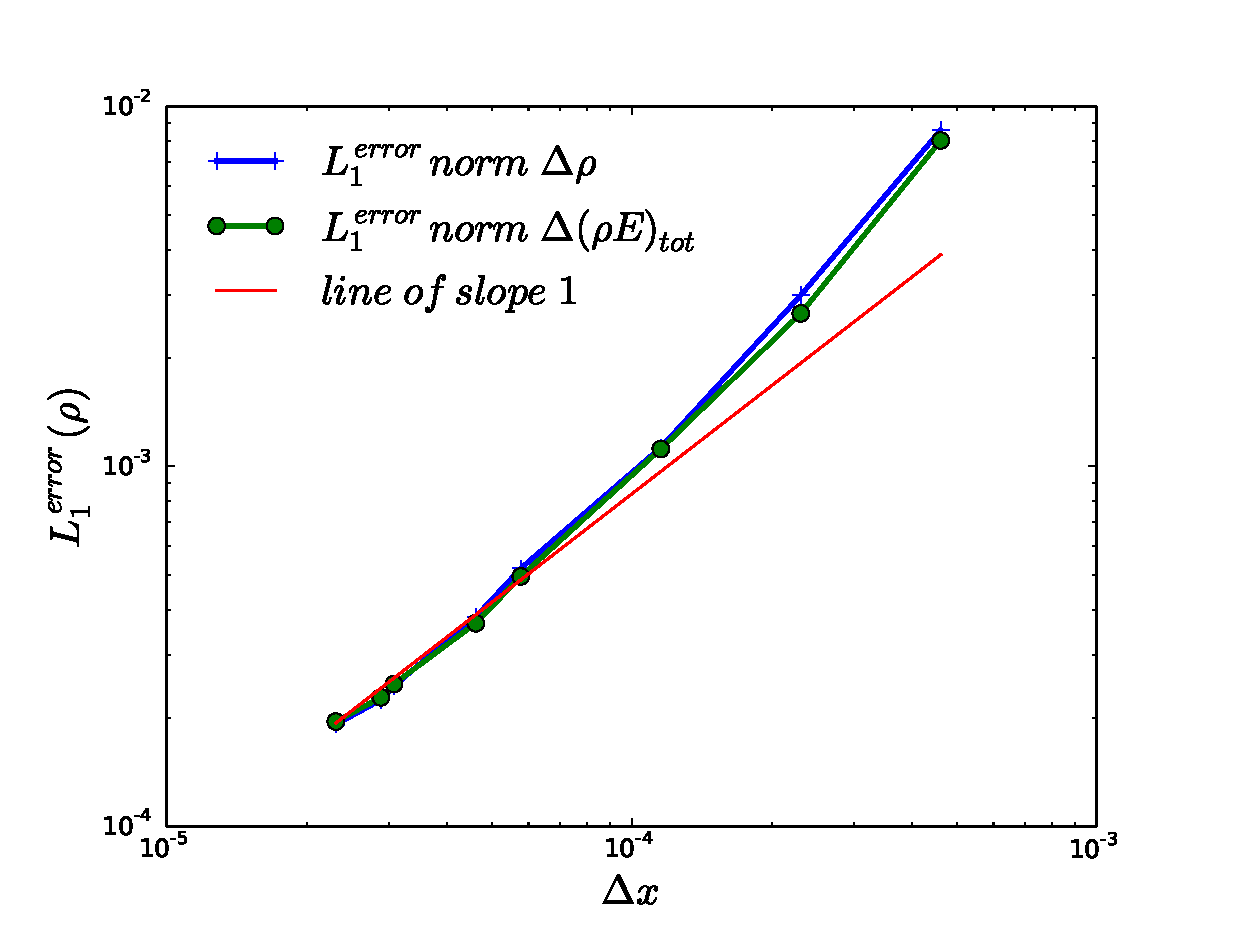
\includegraphics[width=\linewidth]{figures/dpt-xs/mass-energy-diff-scd-method-density-convergence.eps}
    \caption{Material density.}\label{fig:mach-3-dpt-xs-density-conv}
    \end{subfigure}
%
    \begin{subfigure}{0.49\textwidth}    
    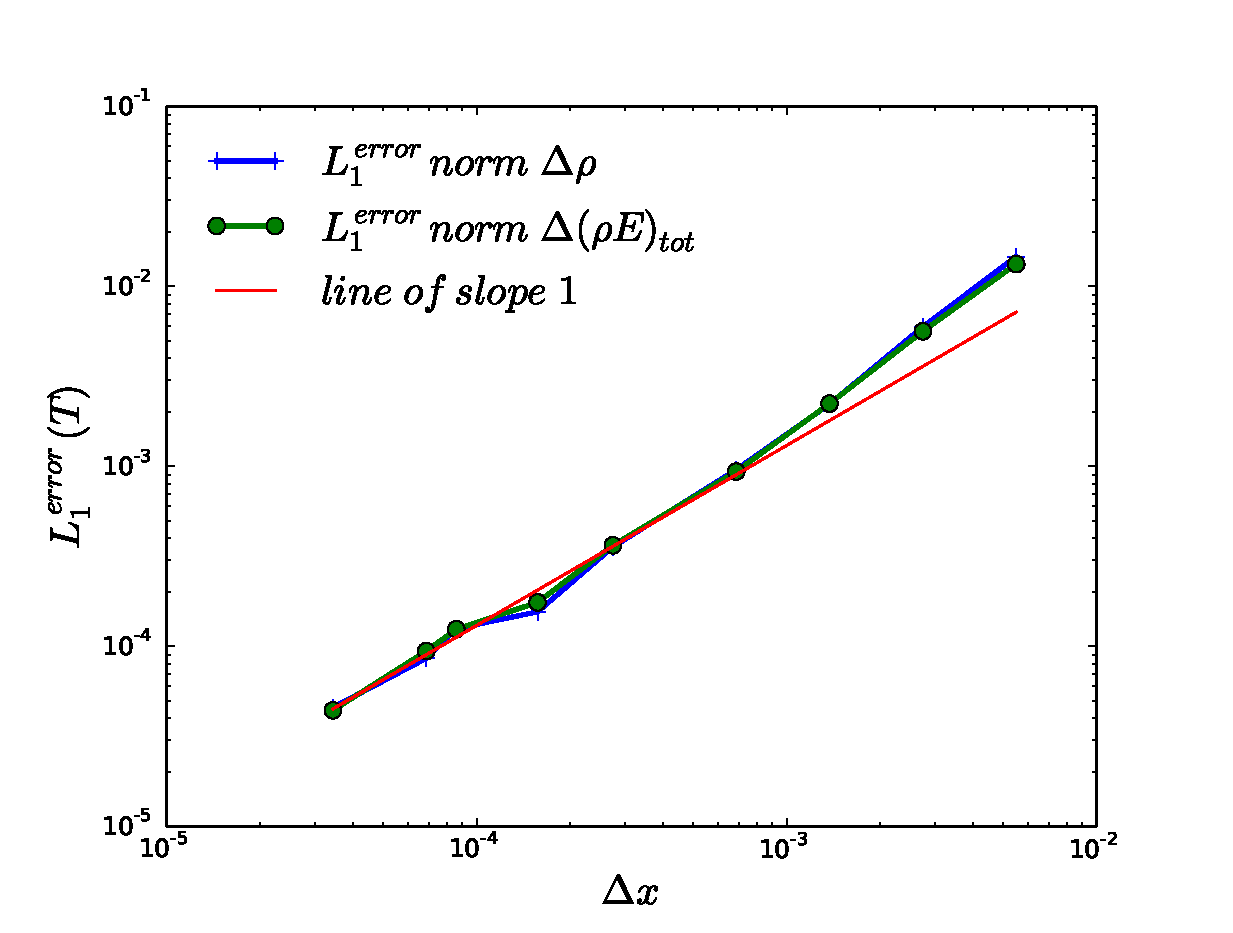
\includegraphics[width=\linewidth]{figures/dpt-xs/mass-energy-diff-scd-method-mat-temp-convergence.eps}
    \caption{Material temperature.}\label{fig:mach-3-dpt-xs-temp-conv}
    \end{subfigure} 
%
    \begin{subfigure}{0.49\textwidth}
    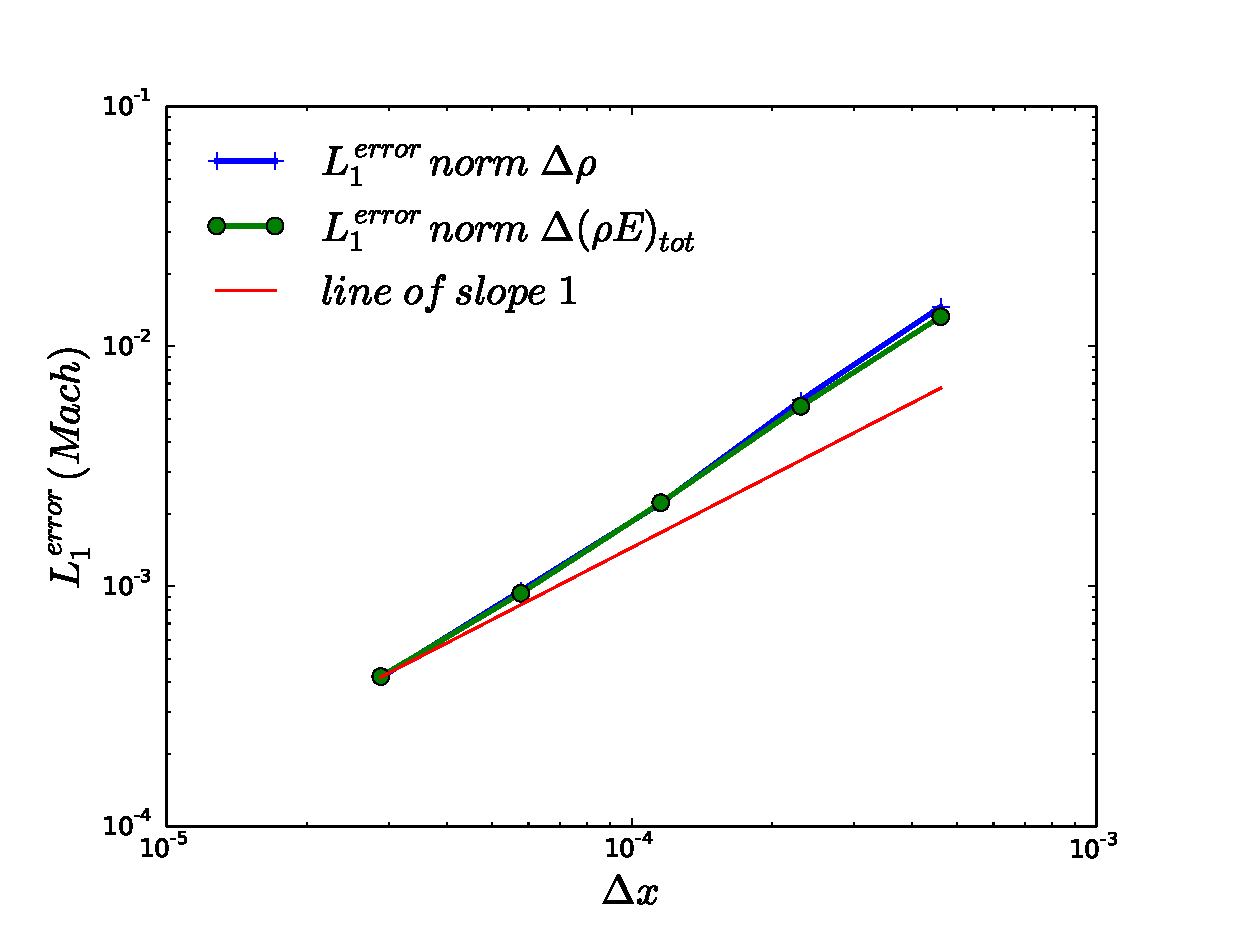
\includegraphics[width=\linewidth]{figures/dpt-xs/mass-energy-diff-scd-method-mach-number-convergence.eps}
    \caption{Mach number.}\label{fig:mach-3-dpt-xs-mach-conv}
    \end{subfigure}
%
    \begin{subfigure}{0.49\textwidth}
    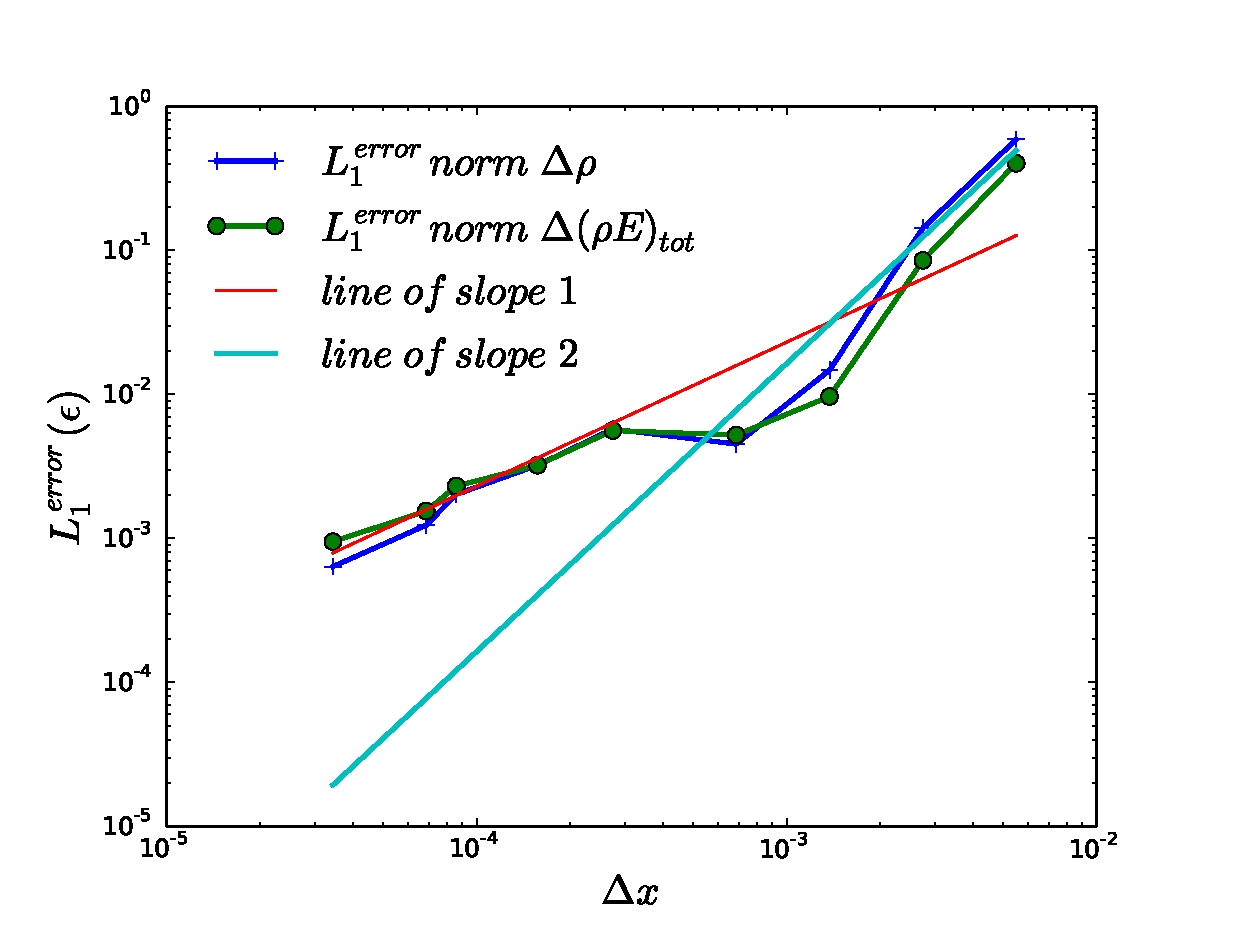
\includegraphics[width=\linewidth]{figures/dpt-xs/mass-energy-diff-scd-method-radiation-convergence.eps}
    \caption{Radiation energy density.}\label{fig:mach-3-dpt-xs-radiation-conv}
    \end{subfigure}        
\caption{Mach $3$ test with density- and temperature-dependent opacity: $L_1$ error norms.}\label{fig:mach-3-dpt-xs-conv} 
\end{figure}
%
\begin{figure}[h]
    \centering
    \begin{subfigure}{0.49\textwidth}
    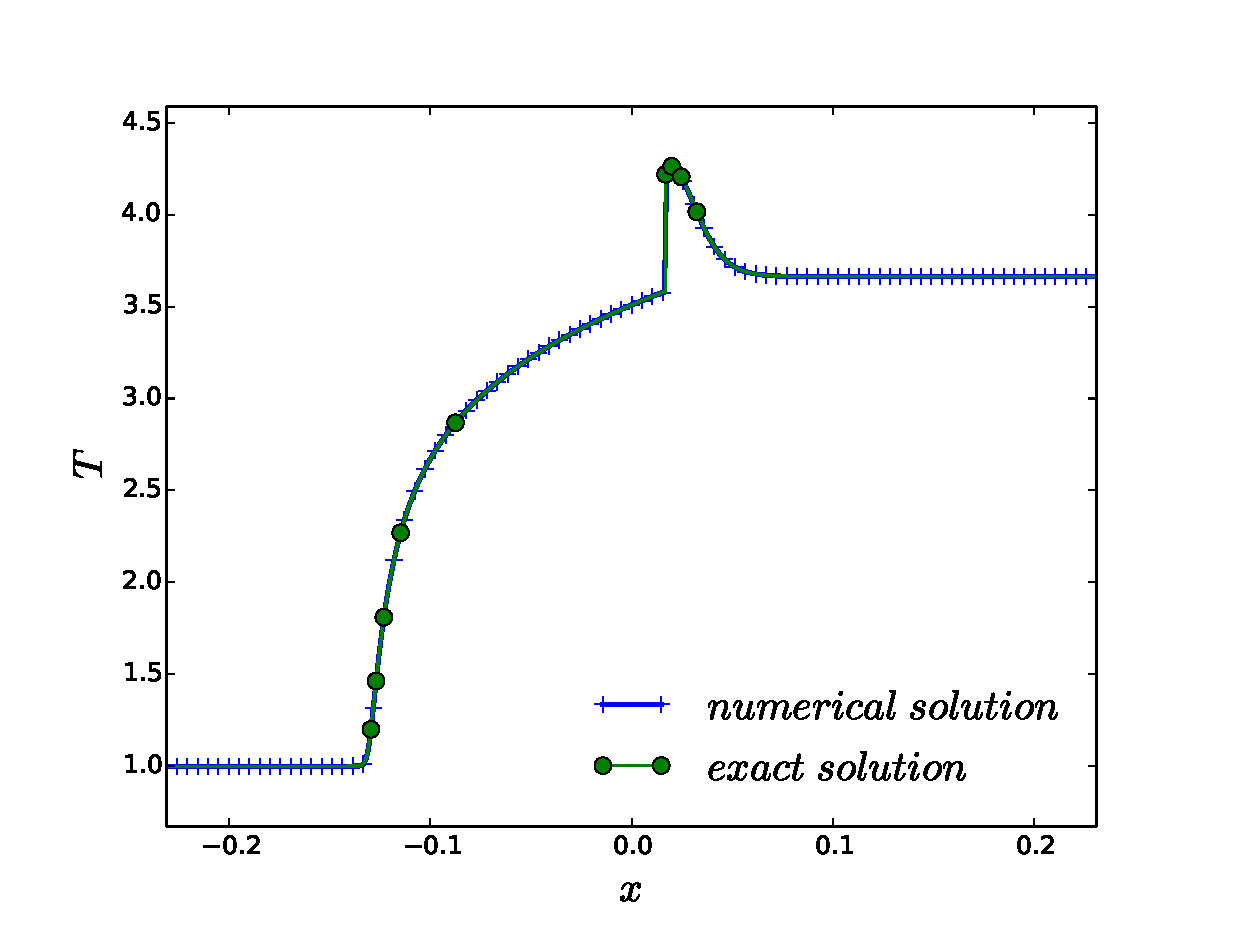
\includegraphics[width=\linewidth]{figures/dpt-xs/mass-diff-mat-temp-nel-2700-plot.eps}
    \caption{Material temperature.}\label{fig:mach-3-dpt-xs-mat-temp}
    \end{subfigure}
%
    \begin{subfigure}{0.49\textwidth}
    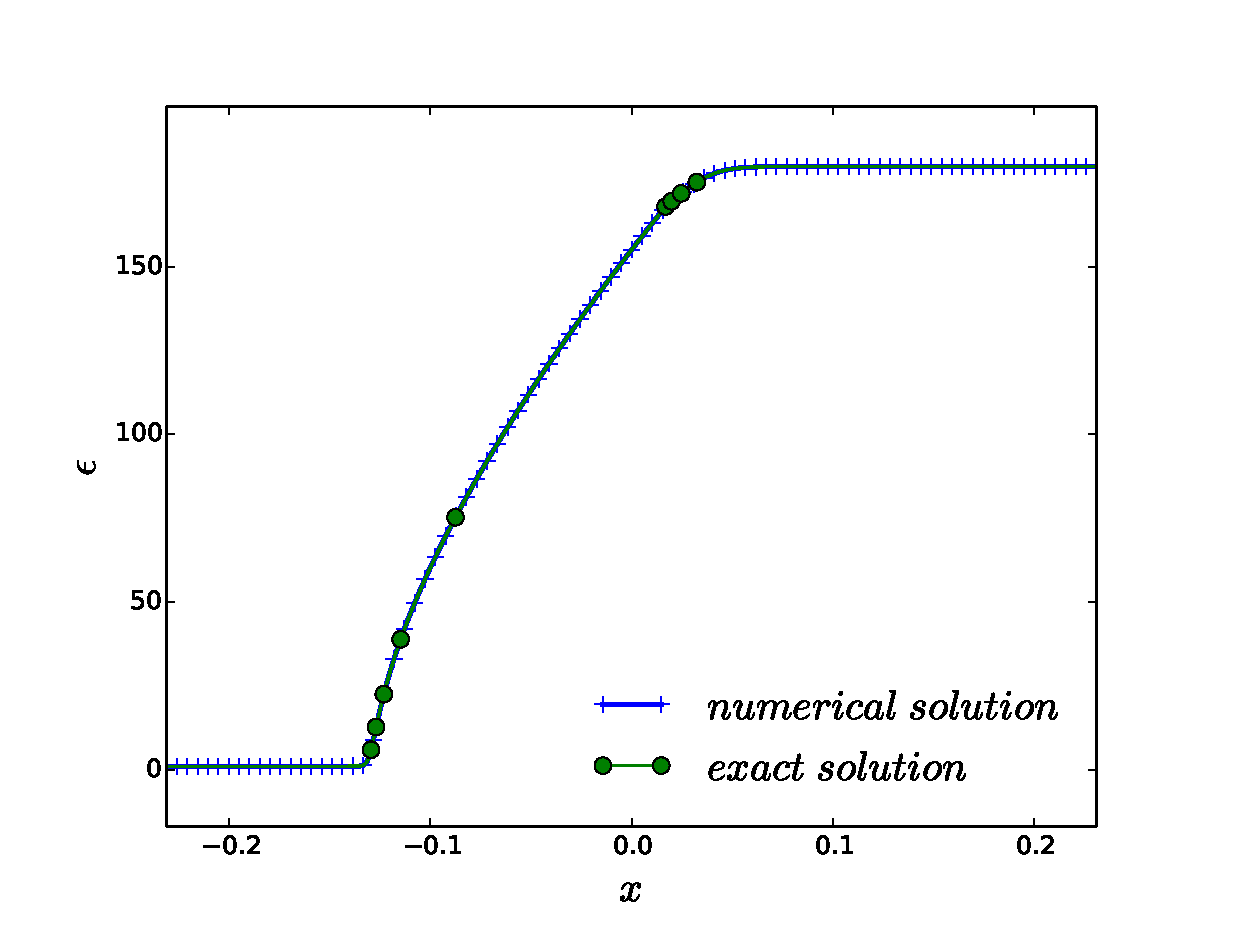
\includegraphics[width=\linewidth]{figures/dpt-xs/mass-diff-radiation-nel-2700-plot.eps}
    \caption{Radiation energy density.}\label{fig:mach-3-dpt-xs-rad-temp}
    \end{subfigure}
%
    \begin{subfigure}{0.49\textwidth}
    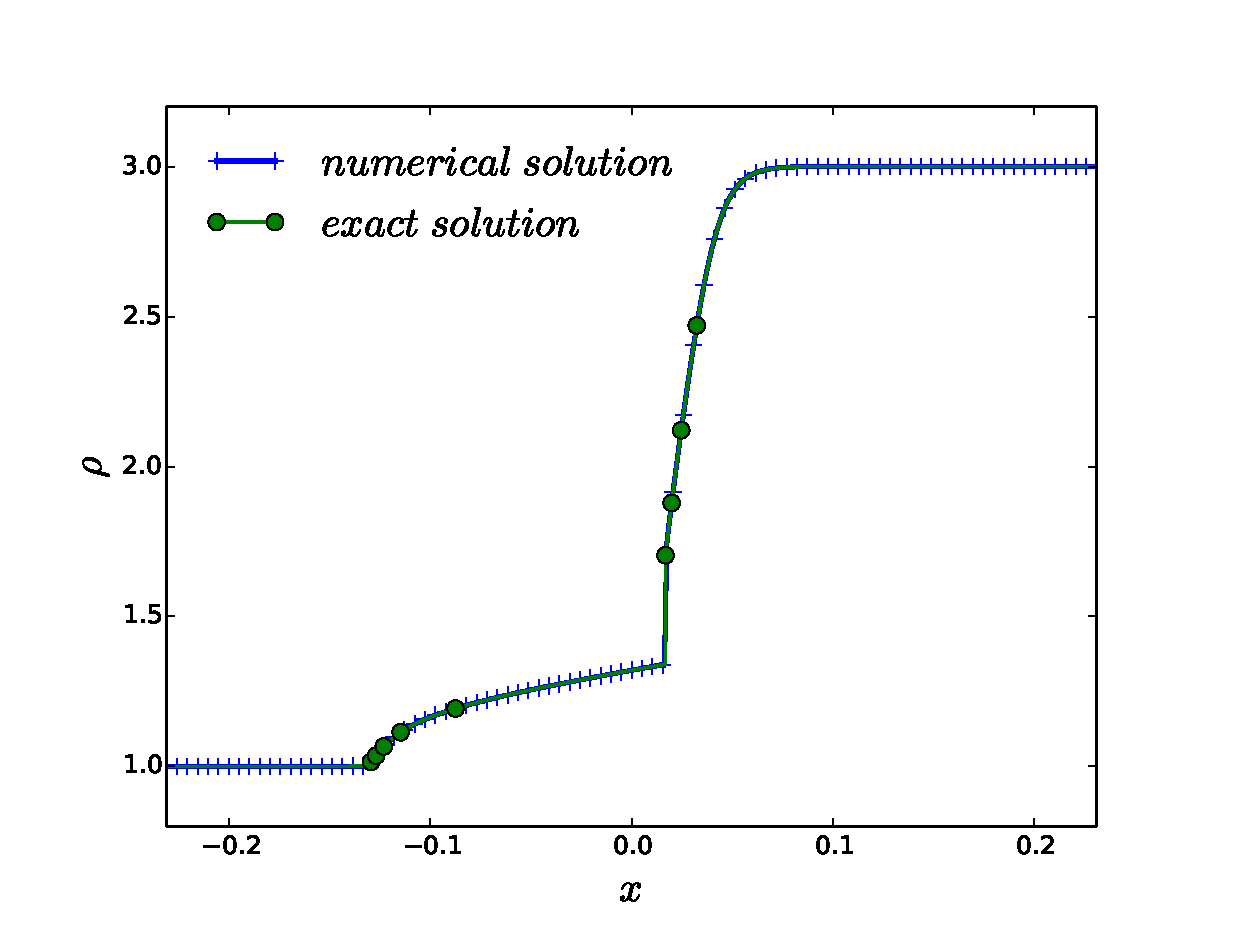
\includegraphics[width=\linewidth]{figures/dpt-xs/mass-diff-density-nel-2700-plot.eps}
    \caption{Material density.}\label{fig:mach-3-dpt-xs-dens}
    \end{subfigure}
%
    \begin{subfigure}{0.49\textwidth}
    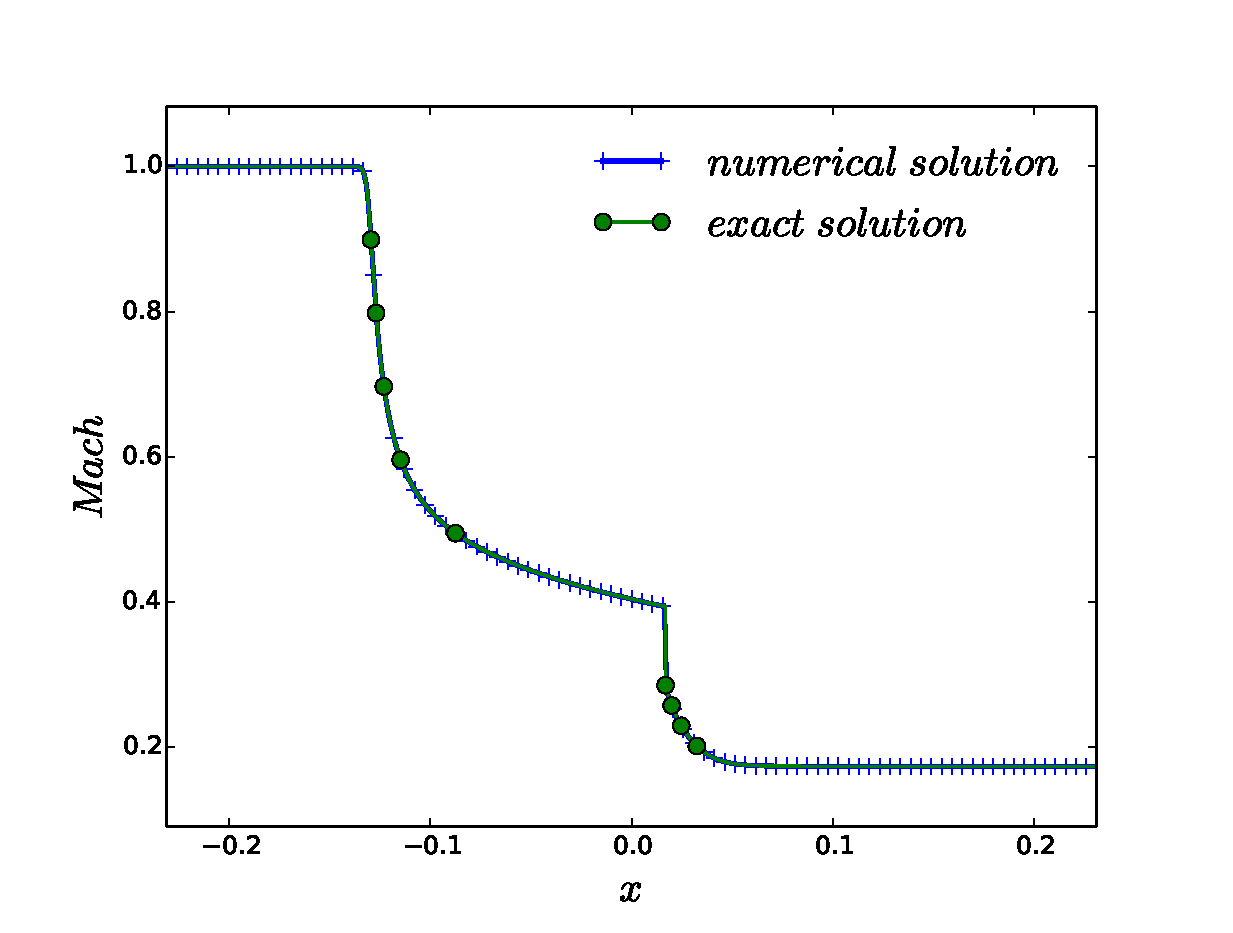
\includegraphics[width=\linewidth]{figures/dpt-xs/mass-diff-mach-number-nel-2700-plot.eps}
    \caption{Mach number.}\label{fig:mach-3-dpt-xs-mach}
    \end{subfigure}
%
    \begin{subfigure}{0.49\textwidth}
    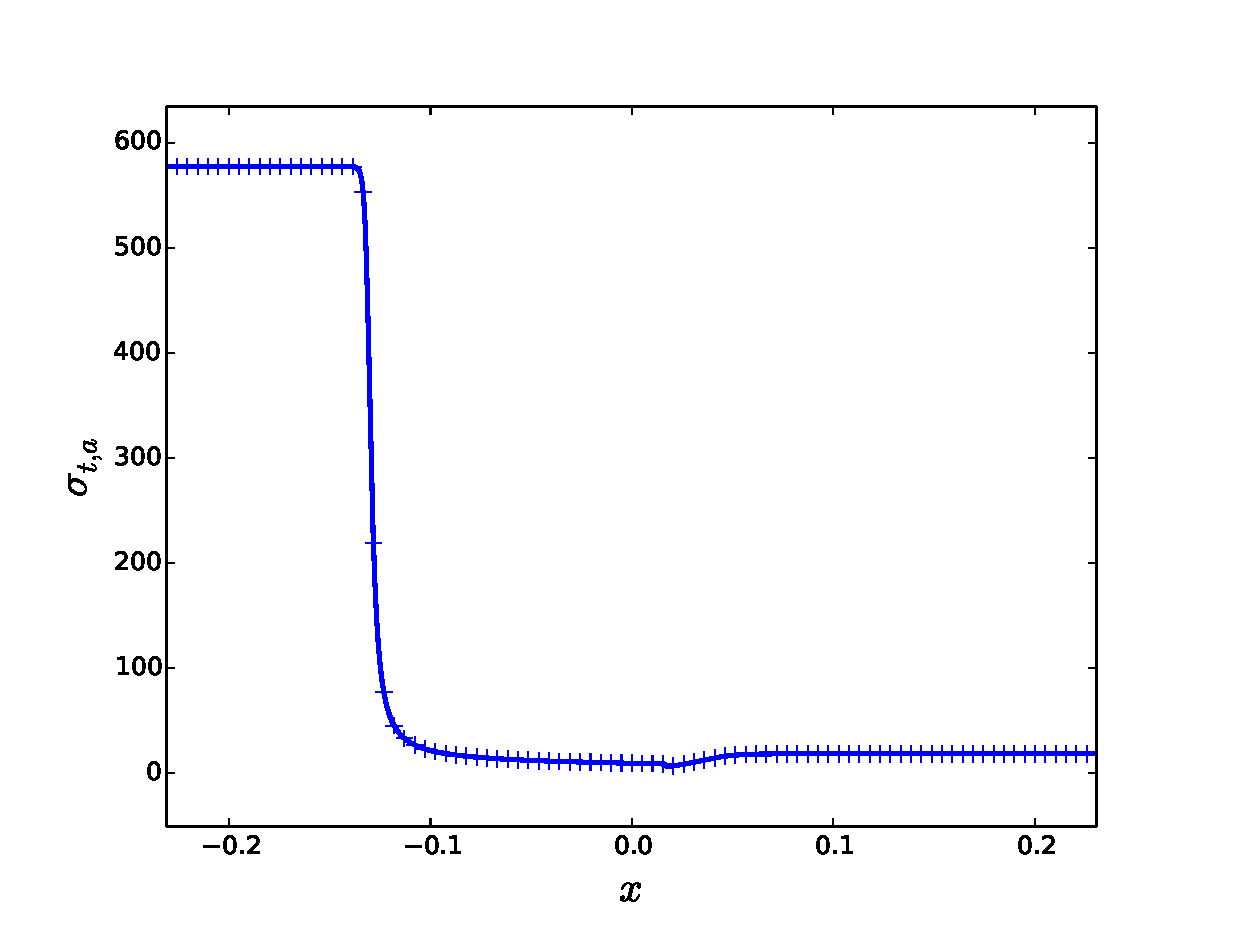
\includegraphics[width=\linewidth]{figures/dpt-xs/mass-diff-opacity-nel-2700-plot.eps}
    \caption{Total opacity $\sigma_t = \sigma_a$.}\label{fig:mach-3-dpt-xs-xs}
    \end{subfigure}
    ~
    \begin{subfigure}{0.49\textwidth}
    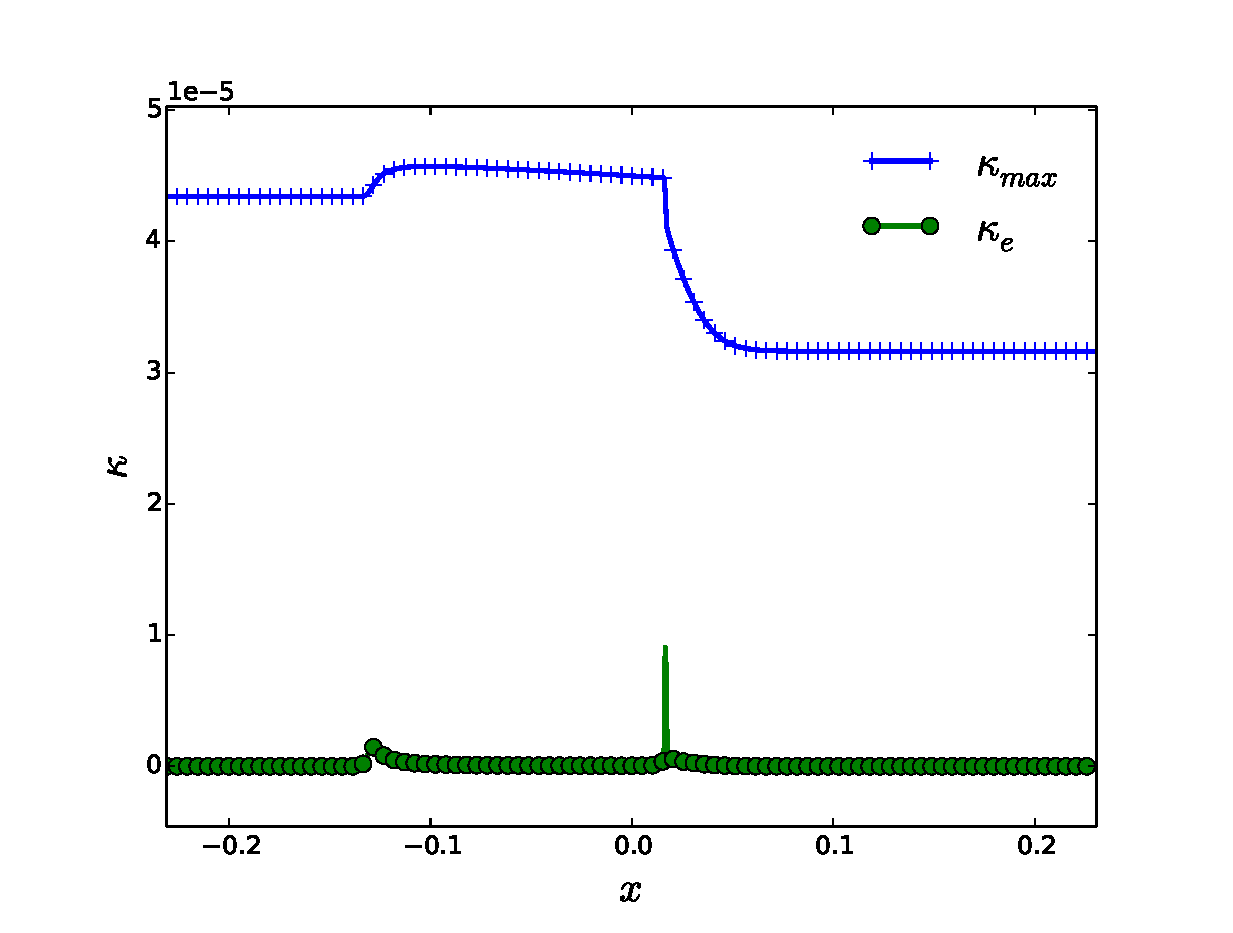
\includegraphics[width=\linewidth]{figures/dpt-xs/mass-diff-visc-nel-2700-plot.eps}
    \caption{Artificial viscosity coefficients.}\label{fig:mach-3-dpt-xs-visc}
    \end{subfigure}      
\caption{Mach $3$ test with density- and temperature-dependent opacity:  Numerical ($2700$ cells) and semi-analytical ($\sim 5 \cdot 10^4$ nodes) steady-state profiles for the material temperature (a), density (b), radiation temperature (c),  Mach number (d), and viscosity coefficient (e).}\label{fig:mach-3-temp-dep-xs}    
\end{figure}
%
The density profile plotted in \fig{fig:mach-3-dpt-xs-dens} does not show any instability neither in the vicinity of the shock around $x \sim 0 \ cm$ nor in the abrupt change located at $x \sim -0.1 \ cm$. The shock is well resolved and the numerical and semi-analytical solutions overlap and are in excellent agreement.
%<<<<<<< HEAD
In \fig{fig:mach-3-dpt-xs-mat-temp} and \fig{fig:mach-3-dpt-xs-rad-temp}, the material and radiation temperatures do not show any instability either. The Zeldovich's spike in the material temperature profile is well resolved. The radiation temperature remains smooth as expected because of the diffusion term in the radiation equation. The numerical and semi-analytical solutions are in excellent agreement. 
%=======
%In \fig{fig:mach-3-dpt-xs-temp}, the material and radiation temperatures do not show any instability either. The Zeldovich spike in the material temperature profile is well resolved. The radiation temperature remains smooth as expected because of the diffusion term in the radiation equation. The numerical and semi-analytical solutions are in excellent agreement. 
%>>>>>>> 80a5074596b6d65166c9c071f44d3b9efb860727
%The numerical profile of the opacity is plotted in \fig{fig:mach-3-dpt-xs-xs} against the semi-analytical solution that was computed from the semi-analytical solutions of the material density and temperature. 
%We recall here that the material is a pure absorber and thus, the total and absorption opacities are equal. The opacity varies by a factor $30$ in the shock region which .... \tcb{Are we not in the case where the material is optically thick in the pre-shock region? If this is the case, we should write something about the interest of using the local entropy residual with a local normalization as we do for Euler equation.}
The profiles of the entropy ($\kappa_e$) and first-order ($\kappa_\text{max}$) viscosity coefficients are showed in \fig{fig:mach-3-dpt-xs-visc}. We observe that the entropy viscosity coefficient $\kappa_e$ displays two peaks at $x\sim-0.1 \ cm$ and at $x \sim 0 \ cm$. The latter one coincides with the shock position where the entropy residual $R_e(x,t)$ is known to be peaked. % (see \sct{sec:def-visc-coeff} and also \cite{our_jcp_radhy_paper}). 
The former one is due to the inclusion of the jumps in the definition of the entropy viscosity coefficient as recalled in \eqt{eq:visc-def}: the material density does not experience a shock at $x\sim-0.1 \ cm$ but a sharp variation that triggers a larger jump value. 
%It is also observed that the entropy viscosity coefficient $\kappa_e$ does not saturate to the first-order viscosity coefficient $\kappa_\text{max}$ in the vicinity of the shock around $x = 0 \ cm$ which can be explained by the dissipative behavior of the source terms that add dissipation as highlighted in \sct{sec:VR_new}. 
Once again, even though the entropy viscosity coefficient $\kappa$ does not saturate to the first-order viscosity coefficient $\kappa_{max}$, the numerical solution is well behaved thanks to the stabilizing effect of the source terms, as explained in \sct{sec:VR_new}.
Overall, the entropy viscosity coefficient behaves as expected: it is peaked in the vicinity of the shock and in regions of sharp variations, and small elsewhere.
%
%------------------------------------------------------------------
%------------------------------------------------------------------
\section{Conclusions and future work}
%------------------------------------------------------------------
%------------------------------------------------------------------
In this paper, the theoretical foundation for the application of the entropy viscosity method to the full non-equilibrium Grey Radiation Hydrodynamic equations, i.e., including relaxation and source terms, has been strengthened, utilizing the notions of weak solution and entropy condition for non-conservative hyperbolic systems of equations. We show that 
(i) we still recover an entropy condition that holds for the full GRH equations when borrowing the functional expression of the entropy  $s(\rho,e,\varepsilon)$ previously derived by only considering the hyperbolic parts of the GRH \cite{our_jcp_radhy_paper}, and
(ii) the same viscous regularization can be employed to stabilize the GRH equations.
%  and, (iii) the asymptotic study of the GRH equations is still equivalent to the equilibrium-diffusion limit (EDL) equations.
Using the above theoretical results, the definition of the first-order and entropy-viscosity coefficients from \cite{our_jcp_radhy_paper} are shown to be still valid. 

The EVM was tested with various test cases and the numerical solutions were compared against semi-analytical solutions obtained by following the method described in \cite{LowrieEdwards}. We proposed a mass and a energy conservation procedures to align numerical and semi-analytical solutions. Convergence studies show that second-order accuracy is obtained for smooth solutions (Mach 1.05 test case) and that solutions with shocks (Mach 3 test cases) yield first-order accuracy in all variables for fine meshes. For the Mach 3 test cases, we also observed that the radiation energy density achieves second order accuracy on coarse meshes (pre-asymptotic region).

Physical features such as embedded hydrodynamic shocks and the Zeldovich spike are resolved accurately without spurious oscillations. The entropy viscosity coefficient is only peaked in the vicinity of the shock and in region of strong gradients, and remains small elsewhere, as expected. Overall, the entropy viscosity method behaves very satisfactorily when compared against semi-analytical solutions.

%The numerical results presented for the Mach 1.05 test case with a pure absorber material showed that second-order accuracy is achieved for smooth solution when compared against a semi-analytical solution. Still using a semi-analytical solution, it was proved that first-order accuracy was achieved for the two Mach-3 radiative shock simulations, with constant and material-dependent opacities, and observed that the entropy viscosity method behaves very satisfactorily when compared against semi-analytical solutions.
%
Future work will include extension to multi-dimensional simulations and the use of an $S_n$ radiation transport approximation to model the radiation energy density distribution.

%%%%%%%%%%%%%%%%%%%%%%%%%%%%%%%%%%%%%%%%%%%%%%%%%%%%%%%%%%%%%
%%%%%%%%%%%%%%%%%%%%%%%%%%%%%%%%%%%%%%%%%%%%%%%%%%%%%%%%%%%%%
\section*{Acknowledgments}
The authors would like to acknowledge Robert Lowrie (LANL), Bojan Popov (TAMU), and Jim Morel (TAMU) for many fruitful discussions.
%%%%%%%%%%%%%%%%%%%%%%%%%%%%%%%%%%%%%%%%%%%%%%%%%%%%%%%%%%%%%
%%%%%%%%%%%%%%%%%%%%%%%%%%%%%%%%%%%%%%%%%%%%%%%%%%%%%%%%%%%%%

\appendix
\section{Implementation of boundary conditions} \label{App:AppendixA}

This appendix deals with the implementation of the boundary conditions for the Grey Radiation-Hydrodynamic equations solved with a \emph{continuous Galerkin finite element method} and with an \emph{implicit temporal solver}. The boundary condition terms arise from the following conservative terms:
%
\begin{equation}\label{eq:bc-fluxes}
F(U) + D(U) = 
\begin{bmatrix}
\rho u \\
\rho u^2 + P + \frac{\epsilon}{3} \\
u \left( \rho E + P \right) \\
\frac{4}{3} u \epsilon
\end{bmatrix}
+  
\begin{bmatrix}
0 \\
0 \\
0 \\
- \frac{c}{3 \sigma_t} \partial_x \epsilon
\end{bmatrix}
\,.
\end{equation}
%
To discretize the conservative fluxes F(U) and D(U) in a finite element approach, one multiplies by a test function $\phi$, and integrates by parts over the computational domain. The resulting boundary terms are as follows:
%
\begin{eqnarray}
\left[\left(F(U)+D(U)\right) \cdot \vec{n} \ \phi \right]_{l} - \left[ \left(F(U)+D(U)\right) \cdot \vec{n} \ \phi \right]_{r} \, ,
\end{eqnarray}
%
where $\vec{n}$ is the outward normal at the left $l$ and right $r$ boundaries.

In the following, we first detail the implementation of the boundary conditions for the first-order differential terms, i.e., advection terms, and then deal with the second-order differential term of the radiation-diffusion equation. 
%
%are wave-dominated equations that require the implementation of boundary conditions consistent with the characteristics. In the finite element approach, boundary terms arise from integrating per part the conservative terms.
%
\subsection{Implementation of the boundary terms from $F(U)$}
%
Study of the hyperbolic term of the 1-D GRH equations yield four eigenvalues that are $\lambda_{1,2}=u$ and $\lambda_{3,4}=u \pm c_m$. The sign of the eigenvalues inform us on how the physical information travel in the computational domain and at the boundaries. We consider in the appendix the cases of a left supersonic and a right subsonic boundaries as they are of interest to the tests presented in this paper. Under the assumption of a supersonic left boundary condition ($u \geq c_m$), all eigenvalues are positive and no physical information leaves the computational domain. As a result, four boundary values, ($\rho_{l, user}, u_{l, user}, P_{l, user}, \epsilon_{l, user})$, must be user-specified and, along with an equation of state, are used to compute the boundary flux $F(U)$. 

In the other hand, the treatment of the right subsonic boundary, ($u \leq c_m$), is quite different as three eigenvalues are positive and one is negative, meaning, physical information leaves and enters the computational domain at the right boundary. Consequently, the right boundary fluxes from the advection terms are computed using one user-specified boundary value, typically the material pressure $P_{r, user}$, and three boundary values supplied by the code, i.e., current values of the material density ($\rho_{r}$) velocity ($u_{r}$) and radiation energy density ($\epsilon_{r}$). Using an equation of state along with the user-specified and current boundary values, the boundary flux $F(U)$ is computed.
%
\subsection{Implementation of the boundary terms from $D(U)$}
%
The radiation-diffusion equation contains the elliptic term $D(U)$ that yields the boundary term 
%
\begin{eqnarray}
\left[D(U)\cdot \vec{n} \ \phi \right]_{l} - \left[D(U)\cdot \vec{n} \ \phi \right]_{r} \, . \nonumber
\end{eqnarray}
%
A reflective boundary condition, i.e. $\left. \partial_x \epsilon \right|_j = 0$, is used to implement the boundary flux from the diffusion term
%
%\begin{eqnarray}
%\partial_x \epsilon = 0 \, ,
%\end{eqnarray}
%
which implies $\left[D(U)\cdot \vec{n} \ \phi \right]_{j} = 0$ for $j = \left( l, \ r \right)$.
%where $\epsilon_{out}$ is a incoming radiation energy density. The above relation allows to derive an expression for the boundary flux $D(U)$ that is function of $\partial_x \epsilon$ (see \eqt{eq:bc-fluxes}):
%
%\begin{eqnarray}
%\left[ \frac{\epsilon}{2} - \frac{\epsilon_{out}}{2} \cdot \vec{n} \ \phi \right]_{j} \text{ with } j = \left( l, \ r \right).
%\end{eqnarray}
% 
%In the continuous Galerkin finite element approach, boundary terms arise from the integration per part of first- and second-order conservative terms. We denote by the fluxes F(U) and D(U) the first- and second-order conservative terms in the 1-D GRH equations, respectively:
%%
%\begin{equation}
%F(U) + D(U) = 
%\begin{bmatrix}
%\rho u \\
%\rho u^2 + P + \frac{\epsilon}{3} \\
%u \left( \rho E + P \right) \\
%\frac{4}{3} u \epsilon
%\end{bmatrix}
%+  
%\begin{bmatrix}
%0 \\
%0 \\
%0 \\
%- \frac{c}{3 \sigma_t} \partial_x \epsilon
%\end{bmatrix}
%\,.
%\end{equation}
%%
%To discretize the conservative flux F(U), one multiplies by a test function $\phi$, integrate over the computational domain and integrate per part. The resulting boundary terms are as follows:
%%
%\begin{eqnarray}
%\left[\left(F(U)+D(U)\right) \cdot \vec{n} \ \phi \right]_{left} - \left[ \left(F(U)+D(U)\right) \cdot \vec{n} \ \phi \right]_{right} \, ,
%\end{eqnarray}
%%
%where $\vec{n}$ is the outward normal.
%\begin{subequations}
%%
%\begin{equation}
%\label{eq:GRHmass}
%\partial_t \left( \rho \right) + \partial_x\left( \rho u \right) = \partial_x \left( \kappa \partial_x \rho \right) \, ,
%\end{equation}
%%
%\begin{equation}
%\label{eq:GRHmom}
%\partial_t \left( \rho u\right) + \partial_x \left(\rho u^2 + P + \frac{\epsilon}{3} \right) = \partial_x \left( \kappa \partial_x \rho u \right) \, ,
%\end{equation}
%%
%\begin{equation}
%\label{eq:GRHenerg}
%\partial_t \left( \rho E\right) + \partial_x \left[ u \left( \rho E + P \right) \right] + \frac{u}{3} \partial_x \epsilon + \sigma_a c \left( \ar T^4 - \epsilon \right) = \partial_x \left( \kappa \partial_x \rho E \right)\, ,
%\end{equation}
%%
%\begin{equation}
%\label{eq:GRHrad}
%\partial_t \epsilon + \frac{4}{3} \partial_x \left( u \epsilon \right) - \frac{u}{3} \partial_x \epsilon - \partial_x \left( \frac{c}{3 \sigma_t} \partial_x \epsilon \right) 
%- \sigma_a c \left( \ar T^4 - \epsilon \right)  = \partial_x \left( \kappa \partial_x \epsilon \right)\, ,
%\end{equation}
%%
%\end{subequations}
%\section{Title of Appendix A} \label{App:AppendixA}
%%%%%%%%%%%%%%%%%%%%%%%%%%%%%%%%%%%%%%%%%%%%%%%%%%%%%%%%%%%%%
%%%%%%%%%%%%%%%%%%%%%%%%%%%%%%%%%%%%%%%%%%%%%%%%%%%%%%%%%%%%%

\bibliography{mybibfile}
\end{document}
